\section{Teoria delle bande e buche di potenziale}

Per sopravvivere dal baratro delle domande d'esame senza risposta, qui scrivo un riassunto che va ripetuto a pappagallo. Subito dopo c'è tutta una sezione dedicata alla spiegazione di codeste strane parole che sembrano messe a caso.

In un atomo isolato gli elettroni possono assumere solo determinati livelli energetici (E1, E2, E3..) che sono i risultati della soluzione dell'equazione di Schrödinger per quel sistema specifico. 

Quando invece un atomo è in presenza di tanti altri atomi dello stesso tipo (come in un reticolo cristallino), questi interagiscono tra loro causando la ramificazione dei livelli di energia formando più livelli con energi poco diverse tra loro, cioè una gamma di valori ammessi che prende il nome di banda di energia. Al posto di livelli discreti, si formano diverse bande.\\
In quest'ultimo caso, le buche di potenziale associate a ciascun nucleo danno luogo ad un potenziale periodico in cui le buche di potenziale corrispondono alla posizione degli atomi.
\subsection{Buca di potenziale in un atomo isolato}
%
Dalla Legge di Coulomb sò che l'energia potenziale tra due cariche è una funzione inversamente proporzionale alla loro distanza.
Considero quindi la struttura di un atomo, in particolare il suo nucleo ed un elettrone (prendiamo come esempio l'atomo di idrogeno). \\
Il sistema costituito da un protone e da un elettrone possiede una certa energia potenziale $U_p(r)$ che posso determinare attraverso la formula del campo elettrico tra due cariche, ottenendo:
\begin{equation*}
    \mathcal{E}(r)=\dfrac{1}{4\pi \epsilon_0} \dfrac{q}{r^2}=k \dfrac{q}{r^2}
\end{equation*}
con $k=\dfrac{1}{4\pi \epsilon_0}$ detta costante di Coulomb.\\
Il potenziale è dato da:
\begin{equation*}
    V(r)=\int_{r}^{\inf}\dfrac{kq}{r^2}dr=\dfrac{kq}{r}
\end{equation*}
dove si è posto la condizione $V(r)=0$ per $r\rightarrow \inf$.\\
Quindi trovo che l'energia potenziale dell'elettrone $U_p(r)$ è dato da:
\begin{equation*}
    U_p(r)=-qV(r)=-\dfrac{kq^2}{r}
\end{equation*}
l'andamento fisico per ($ r>0$) e l'andamento 3D saranno quindi:
\begin{figure}[htb!]
    \centering
    \begin{minipage}[b]{0.49\textwidth}
        \centering
        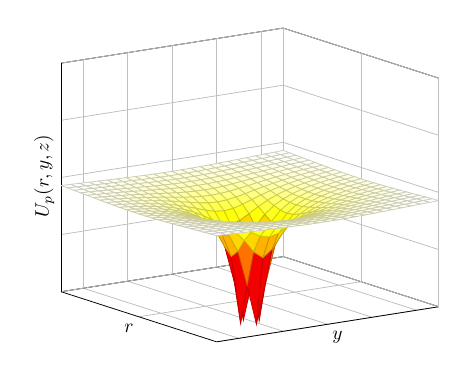
\begin{tikzpicture}[scale=0.7]
    \begin{axis}[
        xlabel={\(r\)},
        ylabel={\(y\)},
        ticks=none,
        zlabel={\(U_p(r,y,z)\)},
        view={55}{15},
        grid=major,
        xmin=-5,
        xmax=5,
        ymin=-5,
        ymax=5,
        zmin=-2,
        zmax=2,
    ]
    \addplot3[
        surf,
        domain=-5:5,
        domain y=-5:5,
        restrict z to domain=-8:1,
        colormap/hot2,
        shader=faceted,
    ] {-1/sqrt(max(x^2 + y^2, 0.01))};
    
    \end{axis}
        \end{tikzpicture}
        \caption{Buca di potenziale di un atomo isolato \\ in 3D}
        \label{fig:Buca di potenziale di un atomo isolato in 3D}
    \end{minipage}%
    \begin{minipage}[b]{0.49\textwidth}
        \centering
       \begin{tikzpicture}[scale=0.45]
        % disegno x
        \draw[->] (0,0) -- (10,0) node[below] {$r$};
        % disegno y
        \draw[->] (0,-5) -- (0,2) node[left] {$U_p(r)$};
        
        % Disegno la curva per r > 0
        \draw[red, domain=0.2:10, samples=100] plot (\x, {-1/\x});
    \end{tikzpicture}
    \caption{Buca di potenziale di un atomo isolato \\ in 2D}
    \label{fig:Buca di potenziale di un atomo isolato in 2D}
    \end{minipage}
    \caption{Buca di potenziale di un atomo isolato}
        \label{fig:Buca di potenziale di un atomo isolato}
\end{figure}
%
\\
Osservando il grafico 3D si può intuire come mai  hanno chiamato questo andamento "buca di potenziale".
Se prendo una sezione 2D avrò quello che molto speso si vede nei testi:
%
\begin{figure}[hbt!]
    \centering
    \includegraphics{Immagini_Micro&Nano/Imm_1_Ripasso/Andamento dell'energia potenziale in un atomo.png}
    \caption{Andamento dell'energia potenziale in un atomo}
    \label{fig:enter_label}
\end{figure}
%
\\
se $r$ è la distanza dell'elettrone dal nucleo dell'atomo allora posso capire che in $r=0$ è situato proprio il nucleodell'atomo.\\
Vedo quindi che per distanze piccole, l'elettrone è prigioniero della buca di potenziale fino a quando non assume abbastanza energia  da superare una soglia e guadagnare la libertà (aka: $U_e > U_{p}(r_1)$).\\
Una considerazione fondamentale in relazione alle buche di potenziale di un atomo siolato è la \textbf{quantizzazione dell'energia}. Questo principio deriva direttamente dall'equazione di Schrödinger e implica che l'energia in un sistema fisico è consentita solo in determinati livelli discreti. \\
Per capire meglio quest'ultima frase, di seguito ho posto una spiegazione. Siccome non sono fisico quantistico, ho trattato la buca di potenziale sotto opportune semplificazioni (visibili nella figura successiva) per affrontarla in maniera più semplice.
%

\begin{citbox}[solo per curiosità]
Si consideri il moto di una particella lungo l'asse $x$; in tale caso la funzione d'onda dipende solo dalla coordinata $x$ e pertanto l'equazione di
Schrédinger può ridursi ad una sola dimensione spaziale.
Si supponga che il moto
della particella non sia libero, ma piuttosto sia confinato da una buca di potenziale ideale di altezza infinita, ossia avvenga in un potenziale pari a 0 per $0<x<d$ e
tendente a $+\inf$ per $x < 0$ e $x > d$:
%
\begin{center}
    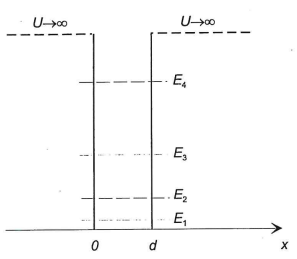
\includegraphics[width=0.25\textwidth]{Immagini_Micro&Nano/Imm_1_Ripasso/Buca di potenziale di altezza infinita.png}
    \captionof{figure}{Buca di potenziale infinita}
\end{center}
%
Poiché il potenziale non dipende
dal tempo si fa uso dell'equazione di Schrédinger per gli stati stazionari in
una dimensione: 
\begin{equation*}
    \dfrac{\hslash^2}{2m}\dfrac{d^2\psi}{dx^2}+(E-U)\psi(x)=0
\end{equation*}
Per risolvere questa equazione studiamo la buca di potenziale per ottenere le condizioni al contorno:
\begin{enumerate}
    \item Per $x<0$ ed $x>d$ l'energia potenziale $U \rightarrow \inf$. Questo si traduce in $\psi=0$, significa che al di fuori della regione della buca di potenziale, la probabilità di trovare la particella è zero. Pertanto, la funzione d'onda, che descrive la probabilità di trovare la particella in una data posizione, deve essere zero al di fuori della buca di potenziale.

    \item Per $0<x<d$ (all'interno della buca di potenziale) vale $U=0$
\end{enumerate}
Detto questo, per garantire la continuità delle funzioni d'onda, all'interno della buca di potenziale ($0<x<d$) dovrà valere $\psi(0)=\psi(d)=0$.
Poniamoci all'interno della buca ($0<x<d$ ed $U=0$), l'equazioni diventa:
\begin{align*}
    \dfrac{\hslash^2}{2m}\dfrac{d^2\psi}{dx^2}+E\psi(x)=0
\end{align*}
La soluzione generale sarà
\begin{equation*}
    \psi(x)=Asin(kx)+Bcos(kx)
\end{equation*}
dove $k=\sqrt{\dfrac{2mE}{\hslash^2}}$\\
Le costanti arbitrarie A e B si determinano imponendo le condizioni al contorno.
Da $\psi(0)=0$ si ottiene $B = 0$; imponendo poi $\psi(d)=0$ risalgo alla condizione $sin(kd)=0$ da cui:
\begin{equation*}
    k=\sqrt{\dfrac{2mE}{\hslash^2}}=\dfrac{n\pi}{d}
\end{equation*}
da cui 
\begin{equation*}
    E=\dfrac{n^2\hslash^2\pi^2}{2md^2}
\end{equation*}
In conclusione l'insieme delle energie permesse è numerabile, e tutte le energie permesse sono multipli interi di un livello fondamentale corrispondente an = 1. Le funzioni d'onda $A sin(kx)$ sono mostrate nella figura sopra . Si noti che a energie crescenti corrisponde un maggior numero di zeri della funzione d'onda (e quindi della probabilità)
all'interno della buca.\\
In generale, lo spettro è continuo in quelle situazioni in cui il moto della particella non
è confinato ad una regione finita dello spazio. Viceversa, lo spettro delle energie e discreto quando il moto della particella è in qualche modo confinato
\end{citbox}
%
\subsection{Buche di potenziale in un reticolo cristallino}
Un solido è formato da tanti atomi posti uno accanto all'altro e, come nel caso isolato, Il nucleo di ciascun atomo crea un campo elettrico ma la differenza è che adesso interagisce con quello degli atomi vicini.
Il risultato sarà che nel solido cristallino, l'energia potenziale creata dall'ammasso di atomi ha forma tridimensionale come nella figura seguente:
%
\begin{figure}[hbt!]
    \centering
    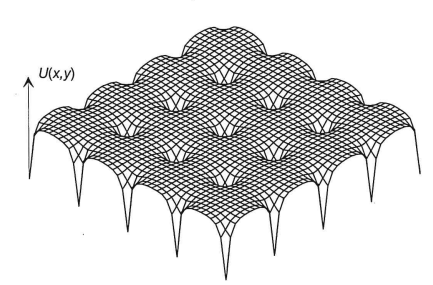
\includegraphics{Immagini_Micro&Nano/Imm_1_Ripasso/Potenziale periodico 3D.png}
    \caption{Potenziale periodico all'interno di un cristallo. 
}
    \label{fig:Potenziale periodico all'interno di un cristallo.}
\end{figure}
\\%
\textbf{La distanza tra due nuclei di due atomi è chiamato "1 Armstrong"}.\\
Come nel caso precedente prendiamo una sezione che passa attraverso i nuclei:
%
\begin{figure}[hbt!]
    \centering
    \includegraphics{Immagini_Micro&Nano/Imm_1_Ripasso/Andamento dell'energia potenziale in un solido.png}
    \caption{Andamento dell'energia potenziale in un solido}
    \label{fig: Andamento dell'energia potenziale in un solido}
\end{figure}
\\%
Dalla figura vedo che la curva non è più asintotica ma presenta un massimo posto a metà tra i due atomi (a metà armstrong).\\
Anche qui faccio delle approssimazioni che mi consentono di vedere le buche in una maniera più intuitiva:
%
FIGURA TA TOGLIERE E CAMBIARE QUELLA SOPRA USANDO LATEX
\begin{figure}[hbt!]
    \centering
    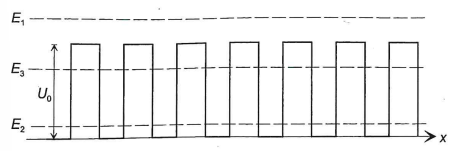
\includegraphics{Immagini_Micro&Nano/Imm_1_Ripasso/Potenziale periodico 2D.png}
    \caption{Potenziale periodico formato da una successione di buche di energia potenziale di altezza finita}
    \label{fig:Potenziale periodico formato da una successione di buche di energia potenziale di altezza finita}
\end{figure}
\\%
Un generico elettrone può trovarsi in diverse situazioni a seconda dell'energia che epossiede:
Io sò che una buca di potenziale può essere vista come un insieme discreto di energie e continue (?).\\
---------------------------------------------------------------------------------------------
Una particella stà all'interno della buca MA, A causa dell'effetto tunnel, le partigelle legate hanno probabilità finita di esistere anche all'esterno della buca.
Consideriamo ora una seconda buca di potenziale, identica, posta a distanza finita dalla prima. Il sistema risultante dalle due buche presenterà sempre un insieme di stati legati, le cui energie non coincideranno però con quelle della buca isolata a
causa del principio di esclusione, ma risulteranno dallo sdoppiamento di queste; vi
sarà poi sempre un insieme continuo di energie corrispondenti a particelle libere. 
...\\
...\\
...\\
----------------------------------------------------------------------------------------------
In una struttura periodica gli elettroni si possono trovare in tre tipi di situazioni:
\begin{enumerate}
    \item elettroni con energia ($E_1 > U_0$, che si muovono come nello spazio libero e non risentono (se non debolmente) della presenza delle buche di potenziale. Si dice che è nello stato libero;

    \item Particelle legate ($E_2 < U_0$, che hanno bassa probabilità di passare da una buca all'altra e pertanto restano confinate, rispettivamente all'interno della propria buca, in modo analogo a quanto accade nel caso di un atomo isolato. Si dice che è nello stato legato al nucleo (di uno degli atomi).

    \item Particelle quasi-libere ($E_3 \approx U_0$), che hanno la possibilità di muoversi per effetto tunnel da una buca di potenziale all'altra e quindi si comportano in modo simile ad una particella libera, ma con relazione fra energia totale $E$ e quantità di moto p diversa da quella della particella libera. Non vado ad indagare oltre (Guione pg 53)
\end{enumerate}
%
Gli elettroni del primo caso, chiamati elettroni liberi,  sono quelli che mi interessano poichè il loro moto forma la corrente elettrica quando vengono sottoposti all'azione di un campo elettrico esterno.\\
Possono quindi muoversi in regioni più distanti dal nucleo, ma continuano comunque ad essere influenzati dalla forza di attrazione elettrostatica con i rispettivi nuclei (ricordo che è una forza elastica).
%
\begin{psbox}[perchè gli elettroni liberi non escono dal solido? sono liberi di uscire dalla buca no?] \label{perchè gli elettroni liberi non escono dal solido?}
    Pur potendosi muovere all'interno del solido, gli elettroni non possono allontanarsene. Tutto funziona come se alla superficie del solido ci fosse una brusca variazione del potenziale che gli elettroni non possono superare se non possiedono la corrispondente energia.
\end{psbox} 
%
 Quando gli atomi si uniscono per formare un cristallo, i livelli energetici degli elettroni degli strati più interni non vengono apprezzabilmente alterati dalla presenza degli atomi vicini, mentre i livelli degli elettroni dell'orbita più esterna risultano cambiati considerevolmente, poichè questi elettroni in un cristallo sono condivisi da più di un atomo.\\
I nuovi livelli energetici degli elettroni esterni possono essere determinati per mezzo della meccanica quantistica e si trova che l'accoppiamento tra gli elettroni dello strato esterno (associato ai livelli d ed f) degli atomi porta come conseguenza la formazione una una banda di livelli energetici poco distanziati tra loro, al posto dei singoli livelli energetici fortemente spaziati presenti nel cso dell'atomo isolato
\begin{figure}[hbt!]
    \centering
    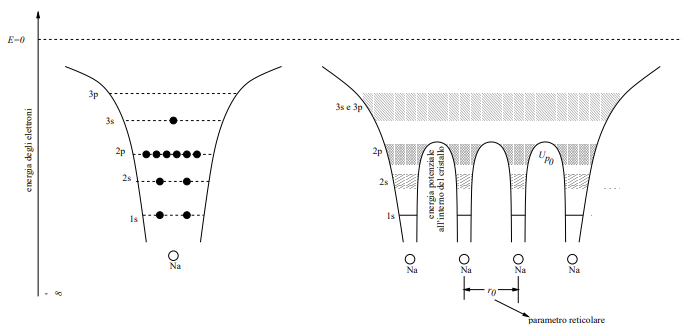
\includegraphics{Immagini_Micro&Nano/Imm_1_Ripasso/Bande di energie nel caso isolato VS solido.png}
    \caption{Livelli energetici nel caso di atomo isolato VS livelli energetici nel caso di un solido}
    \label{fig:Livelli energetici nel caso di atomo isolato VS livelli energetici nel caso di un solido}
\end{figure}
%
\\
Adesso voglio sapere come si formano le bande di energia.\\

consideriamo un sistema costituito da due soli atomi. 
Per entrambi gli atomi consideriamo solo l'elettrone che occupa il livello di energia più elevato (cioè quello più esterno; i chimici li chiamano d o f), trascurando i livelli occupati di energia inferiore.\\
Quando due atomi sono separati da una distanza così grande da poterli considerare isolati, l'elettrone associato a ciascun atomo possiede un'energia di valore $E_n$ soluzione dell'equazione di Schrodinger (spiegato prima).\\
Se la distanza di separazione è ridotta, un elettrone sarà soggetto a una forza dovuta alla presenza del secondo nucleo. Il potenziale che determina i livelli di energia dell'elettrone risulta quindi modificato e così pure lo spettro dei possibili valori di energia. Per descrivere un sistema di due atomi devo usare il principio di esclusioen di paoli. In condizioni normali ogni atomo isolato ha un livello di energia En che può ospitare al massimo due elettroni con spin opposto, limitando il sistema a un massimo di quattro elettroni.
%
\begin{psbox}[l'ultima frase è spiegata male]
    Nel caso di un singolo atomo isolato, un livello di energia (denotato come En) può ospitare al massimo due elettroni, ciascuno con spin opposto. Quindi, se prendiamo due atomi isolati, il numero massimo di elettroni che possono occupare il livello En è 4 (2 nel primo atomo e 2 nel secondo).
    RIVERE QUESTA SEZIONE
\end{psbox}
%
 Tuttavia, quando i due atomi si avvicinano a formare un unico sistema, il livello di energia consentito En può ora ospitare solo due elettroni. Quindi il livello di energia En relativo a ciascun atomo isolato si sdoppierà in due livelli, di energia leggermente differente, al fine di garantire la coesistenza di quattro elettroni.\\
L'effetto dell'iterazione tra i due atomi è di perturbare il valore di energia relativo al livello considerato dell'atomo isolato e di indurreuno sdoppiamento dei livelli di energia perturbati.\\
Avvicinando ulteriormente i due atomi, la perturbazione dovuta all'avvicinamento è maggiore, come pure la differenza di energia tra i livelli sdoppiati.\\
Raggruppando più atomi di una struttura scristallina, le forze cui sono soggetti gli elettroni sono ulteriormente modificate e così pure i valori di energia permessi.\\
---------------\\
Anche qui, il principio di esclusione di Pauli richiede che
ciascun livello permesso abbia un'energia di valore leggermente diverso, cosicchè il cristallo risulta caratterizzato
da numerosi livelli, tutti distinti in energia ma molto prossimi tra loro. Ogni livello quantizzato corrispondente
all'atomo isolato si scinde in più livelli, ciascuno corrispondente a un atomo nel sistema. Se il sistema è composto
da N atomi, l'originario livello di energia En si scinde in N livelli permessi, costituenti una banda di energia
che contiene al più 2N elettroni.\\ 
Poichè il numero di atomi in un cristallo è molto grande (dell'ordine di $10^{22} cm^{-3}$) e l'estensione della banda di energia è dell'ordine di pochi eV, gli N livelli distinti componenti le bande sono separati da intervalli di energia assai più piccoli dell'energia termica di un elettrone a temperatura ambiente, cosicchè l'elettrone può agevolemnte effettuare transizioni tra i livelli. Si può quindi parlare di una banda continua di valori di energia permessi, occupabile al più da 2N elettroni.
%
\begin{figure}[hbt!]
    \centering
    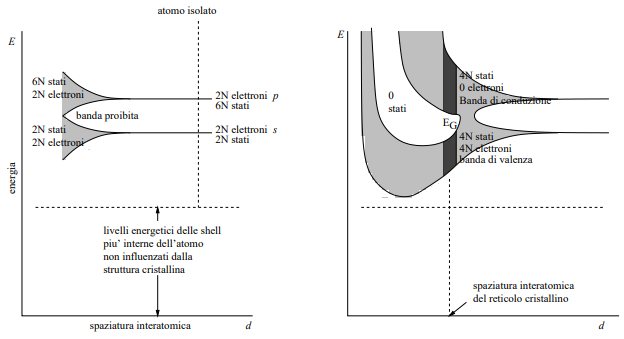
\includegraphics{Immagini_Micro&Nano/Imm_1_Ripasso/bande di energia.png}
    \caption{Banda di energia che si forma in un reticolo cristallino}
    \label{fig:Banda di energia che si forma in un reticolo cristallino}
\end{figure}
%

Quindi i livelli discreti di energia-dell'atomo isolato si trasformano in bande di energia permessa separate da bande proibite.\\
Le bande di energia interessanti ai fini del comportamento-chimico ed elettrico sono quelle superiori: la banda contenente gli elettroni di valenza, quelli cioè più esterni, che contribuiscono
ai legami chimici, è detta banda di valenza mentre la banda immediatamente superiore si dice banda di conduzione. \\
Si può assumere come estremo superiore della banda di conduzione il livello del vuoto; al livello del vuoto corrisponde l'energia minima che un elettrone deve possedere per sfuggire all'esterno del solido. Per energie maggiori del livello del vuoto l'elettrone è libero e la sua energia presenta uno spettro continuo. All'interno di ciascuna banda (valenza o conduzione) la relazione di dispersione dell'elettrone si può in molti casi approssimare con una forma parabolica analoga alla relazione di dispersione di un elettrone
nello spazio libero; la relativa massa efficace m* si indicherà con m;, per gli elettroni della banda di conduzione e con —mj, per gli elettroni della banda di valenza,
per motivi che diventeranno chiari in seguito. \\

La buca di potenziale è una zona di spazio circondata da un elevato campo elettrico. in un atomo gli elettroni dell'atomo vedono il nucleo posto al centro di una buca di potenziale.
%
\subsection{Dentro la lezione di microelettronica: struttura a bande}
La sezione precedente aveva lo scopo di spiegare dando un'idea di quello che succede nel reticolo cristallino e servirà anche per rispondere a dubbi che si creeranno leggendo questa sezione.\\
Qui rifaremo le medesime osservazioni ma sotto opportune semplificazioni visive per rendere il problema matematicamente trattabile.\\

All'interno della bucha di potenziale, un elettrone ha la possibilità di muoversi liberamente. Tuttavia, se l'elettrone acquista abbastanza energia cinetica e si allontana notevolmente dal centro dell'atomo, può superare la forza di attrazione e, di conseguenza, "uscire" dalla regione di influenza dell'atomo.\\
Questo fenomeno può essere spiegato attraverso i principi della meccanica quantistica, in cui la posizione dell'elettrone è descritta dalla funzione d'onda e la sua probabilità di trovarsi in diverse posizioni è governata dalle leggi della teoria quantistica.\\

Le buche di potenziale più esterne dal reticolo cristallino vengono rappresentate con pareti di potenziale infinite (vedi sezione \ref{perchè gli elettroni liberi non escono dal solido?}) mentre ciascuna delle buche interne al solido può essere modellata come come una buca di potenziale con con pareti limitate non infinite, dove la parete della buca di potenziale di un atomo viene chiusa dalla parete della buca di potenziale dell'atomo accanto (vedi Figura \ref{fig: Andamento dell'energia potenziale in un solido}):

\begin{figure}[htb!]
    \centering
    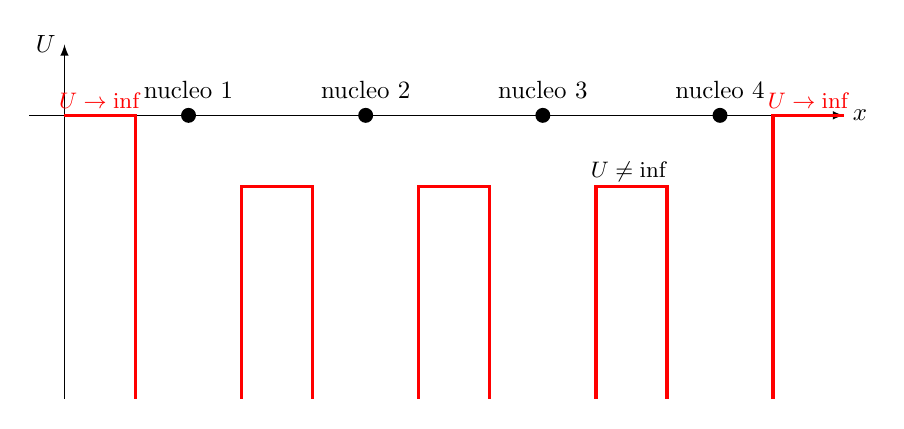
\begin{tikzpicture}[scale=0.9, transform shape]
        %disegno asse x
        \draw[-latex] (-0.5,0)-- (11,0) node[right]{$x$};
        %disegno asse y
        \draw[-latex] (0,-4)-- (0,1) node[left]{$U$};
        %disegno buche e label potenziale
        \draw[very thick,red] (0,0)--++ (1,0)--++ (0,-4);
        \draw[very thick,red] (2.5,-4)--++ (0,3)--++ (1,0)--++ (0,-3);
        \draw[very thick,red] (5,-4)--++ (0,3)--++ (1,0)--++ (0,-3);
        \draw[very thick,red] (7.5,-4)--++ (0,3)--++ (1,0)--++ (0,-3);
        \draw[very thick,red] (10,-4)--++ (0,4)--++ (1,0);
        \node at (-0.2,0.2)[right,red]{\small{$U\rightarrow \inf$}};
        \node at (9.8,0.2)[right,red]{\small{$U\rightarrow \inf$}};
        \node at (7.97,-0.8)[thick]{\small{$U \neq \inf$}};
        %disegno i nuclei 
        \node[circle,fill=black,inner sep=0pt,minimum size=6pt,label=nucleo 1] at (1.75,0) {};
        \node[circle,fill=black,inner sep=0pt,minimum size=6pt,label=nucleo 2] at (4.25,0) {};
        \node[circle,fill=black,inner sep=0pt,minimum size=6pt,label=nucleo 3] at (6.75,0) {};
        \node[circle,fill=black,inner sep=0pt,minimum size=6pt,label=nucleo 4] at (9.25,0) {};
       
    \end{tikzpicture}
    \caption{Buche di potenziale in un solido-Le più esterne hanno pareti con potenziale infinito}
    \label{fig:Buche di potenziale in un solido-Le più esterne hanno pareti con potenziale infinito}
\end{figure}
%
\noindent\begin{minipage}{0.6\textwidth}% adapt widths of minipages to your needs
Ricordo che se la parete di potenziale è infinita, i livelli energetici ammessi sono discreti e di valore:
\begin{equation*}
    E_n=\dfrac{n^2\hslash^2 \pi^2}{2md}
\end{equation*}
dove d è la distanza tra le pareti della buca.
Si noti come l'energia dipende solo dalla distanza tra le pareti mentre \textbf{l'altezza della buca non entra in gioco} perchè l'altezza della buca è infinita.
Se le pareti fossero finite (\textbf{aka: $U \neq \inf$}), si otterrebbero dei livelli che vanno come:
\begin{equation*}
    E_u=n^2h\pi^2
\end{equation*}
\end{minipage}%
\hfill%
\begin{minipage}{0.3\textwidth}
\begin{center}
    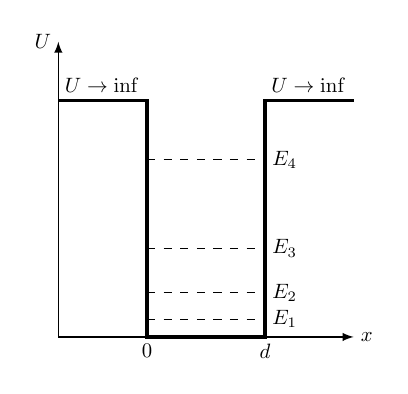
\begin{tikzpicture}[scale=0.75,transform shape]
        %disegno asse x
        \draw[-latex] (0,0)-- (5,0) node[right]{$x$};
        %disegno asse y
        \draw[-latex] (0,0)-- (0,5) node[left]{$U$};
        %disegno buche
        \draw[very thick,black] (0,4)--++ (1.5,0) node[anchor=south east]{$U\rightarrow \inf$} --++ (0,-4)--++ (2,0)--++ (0,4)--++ (1.5,0) node[anchor=south east]{$U\rightarrow \inf$};
        %livelli energetici
        \draw[dashed] (1.5,0.30)--++ (2,0) node[right]{$E_1$};
        \draw[dashed] (1.5,0.75)--++ (2,0) node[right]{$E_2$};
        \draw[dashed] (1.5,1.5)--++ (2,0) node[right]{$E_3$};
        \draw[dashed] (1.5,3)--++ (2,0) node[right]{$E_4$};
        %label
        \node at (1.5,0)[below]{$0$};
        \node at (3.5,0)[below]{$d$};
    \end{tikzpicture}
    \captionof{figure}{buca di potenziale con pareti infinite}
    \label{fig:buca di potenziale con pareti infinite}
\end{center}
\end{minipage}
Nel caso di pareti finite è più difficile trovare i valori in forma chiusa dei livelli di energia discreti (E1,E2,E3..) ma la cosa più importante è un'altra:
Nelle buche di potenziale a pareti infinite, la probabilità di trovare un elettrone all'interno della buca di potenziale ha una funzione d'onda $\psi_1, \psi_2,\psi_3$ tale per cui 
\begin{equation}
    \sum_i \int \left| \psi_i\right|^2 dx=1
\end{equation}
\\%
Questa cosa la posso tradurre come "nel caso infinito ho che per x<0 e x>d ho probabilità nulla fuori dalla buca e probabilità certa dentro la buca".\\
Nel caso di pareti finite la situazione cambia dato che si può osservare una probabilità diversa da zero che di trovare l'elettrone fuori e \textbf{questo è il concetto proveniente dalla meccanica quantistica che ci portiamo dietro}.\\
%
\noindent\begin{minipage}{0.49\textwidth}% adapt widths of minipages to your needs
\begin{center}
    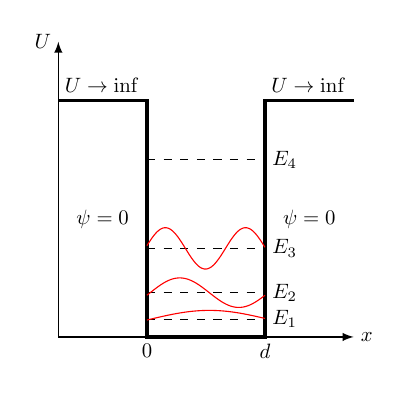
\begin{tikzpicture}[scale=0.75,transform shape]
        %disegno asse x
        \draw[-latex] (0,0)-- (5,0) node[right]{$x$};
        %disegno asse y
        \draw[-latex] (0,0)-- (0,5) node[left]{$U$};
        %disegno buche
        \draw[very thick,black] (0,4)--++ (1.5,0) node[anchor=south east]{$U\rightarrow \inf$} --++ (0,-4)--++ (2,0)--++ (0,4)--++ (1.5,0) node[anchor=south east]{$U\rightarrow \inf$};
        %livelli energetici
        \draw[dashed] (1.5,0.30)--++ (2,0) node[right]{$E_1$};
        \draw[dashed] (1.5,0.75)--++ (2,0) node[right]{$E_2$};
        \draw[dashed] (1.5,1.5)--++ (2,0) node[right]{$E_3$};
        \draw[dashed] (1.5,3)--++ (2,0) node[right]{$E_4$};
        %label
        \node at (1.5,0)[below]{$0$};
        \node at (3.5,0)[below]{$d$};
        %plot funzioni psi
        \draw[red, domain=1.5:3.5, samples=200, smooth] plot (\x, {0.3+0.15*sin(90*\x+220))});
        \draw[red, domain=1.5:3.5, samples=200, smooth] plot (\x, {0.75+0.25*sin(180*\x+80))});
        \draw[red, domain=1.5:3.5, samples=200, smooth] plot (\x, {1.5+0.35*sin(265*\x-30))});
        %
        \node at (0.75,2)[align=center]{$\psi = 0$};
        \node at (4.25,2)[align=center]{$\psi = 0$};
        \end{tikzpicture}
    \captionof{figure}{buca di potenziale con pareti infinite, l'elettrone è confinato nella buca}
    \label{fig:buca di potenziale con pareti infinite v2}
\end{center}
\end{minipage}%
\hfill%
\begin{minipage}{0.49\textwidth}
\begin{center}
    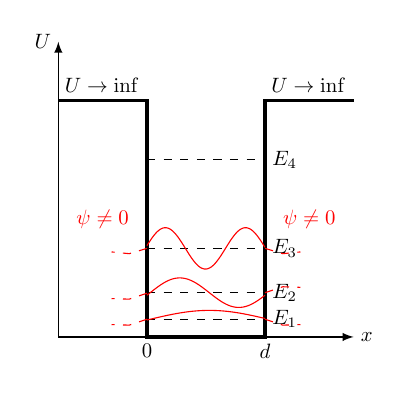
\begin{tikzpicture}[scale=0.75,transform shape]
        %disegno asse x
        \draw[-latex] (0,0)-- (5,0) node[right]{$x$};
        %disegno asse y
        \draw[-latex] (0,0)-- (0,5) node[left]{$U$};
        %disegno buche
        \draw[very thick,black] (0,4)--++ (1.5,0) node[anchor=south east]{$U\rightarrow \inf$} --++ (0,-4)--++ (2,0)--++ (0,4)--++ (1.5,0) node[anchor=south east]{$U\rightarrow \inf$};
        %livelli energetici
        \draw[dashed] (1.5,0.30)--++ (2,0) node[right]{$E_1$};
        \draw[dashed] (1.5,0.75)--++ (2,0) node[right]{$E_2$};
        \draw[dashed] (1.5,1.5)--++ (2,0) node[right]{$E_3$};
        \draw[dashed] (1.5,3)--++ (2,0) node[right]{$E_4$};
        %label
        \node at (1.5,0)[below]{$0$};
        \node at (3.5,0)[below]{$d$};
        %plot funzione psi E1
        \draw[red,dashed] (1.5,0.3)--++ (-0.3,-0.1)--++ (-0.3,0.01);
        \draw[red, domain=1.5:3.5, samples=200, smooth] plot (\x, {0.3+0.15*sin(90*\x+220))});
        \draw[red,dashed] (3.5,0.3)--++ (0.3,-0.1)--++ (0.3,0.01);
        %plot funzione psi E2
         \draw[red,dashed] (1.5,0.74)--++ (-0.3,-0.1)--++ (-0.3,0.01);
        \draw[red, domain=1.5:3.5, samples=200, smooth] plot (\x, {0.75+0.25*sin(180*\x+80))});
        \draw[red,dashed] (3.5,0.75)--++ (0.3,+0.1)--++ (0.3,-0.01);
        %plot funzione psi E3
         \draw[red,dashed] (1.5,1.5)--++ (-0.3,-0.09)--++ (-0.3,0.03);
        \draw[red, domain=1.5:3.5, samples=200, smooth] plot (\x, {1.5+0.35*sin(265*\x-30))});
        \draw[red,dashed] (3.5,1.5)--++ (+0.3,-0.09)--++ (+0.3,0.03);
        %
        \node at (0.75,2)[align=center,red]{$\psi \neq 0$};
        \node at (4.25,2)[align=center,red]{$\psi \neq 0$};
    \end{tikzpicture}
    \captionof{figure}{buca di potenziale con pareti finite, non è detto che l'elettrone sia confinato nella buca}
    \label{fig:buca di potenziale con pareti finite}
\end{center}
\end{minipage}
\\%
Da qui si scatena un'altro ragionamento:
Io sò che per ogniuno di questi livelli energetici (e1, e2...) il principio di esclusione di paoli sancisce che due elettroni non possono avere lo stesso stato energetico a meno che non abbiano spin opposto.\\
Allora succede che nel momento in cui atomi isolati cominciano ad unirsi formando il reticolo cristallino, elettroni che appartengono a buche adiacenti hanno probabilità diversa da zero di esistere nei livelli energetici degli atomi accanto.
Se nucleo 1 ha 1 elettrone e nucleo 3 ha un altro elettrone, allora la probabilità di trovare questi due dentro il nucleo 2 è diversa da zero.
Questo è legato al fatto che siccome le buche non hanno pareti infinite, allora la funzione d'onda si espande fuori dalla buca.
\begin{figure}[htb!]
    \centering
    \begin{tikzpicture}
        %disegno asse x
        \draw[-latex] (-0.5,0)-- (11,0) node[right]{$x$};
        %disegno asse y
        \draw[-latex] (0,-4)-- (0,1) node[left]{$U$};
        %disegno buche e label potenziale
        \draw[very thick,red] (0,0)--++ (1,0)--++ (0,-4);
        \draw[very thick,red] (2.5,-4)--++ (0,3)--++ (1,0)--++ (0,-3);
        \draw[very thick,red] (5,-4)--++ (0,3)--++ (1,0)--++ (0,-3);
        \draw[very thick,red] (7.5,-4)--++ (0,3)--++ (1,0)--++ (0,-3);
        \draw[very thick,red] (10,-4)--++ (0,4)--++ (1,0);
        \node at (-0.2,0.2)[right,red]{\small{$U\rightarrow \inf$}};
        \node at (9.8,0.2)[right,red]{\small{$U\rightarrow \inf$}};
        \node at (7.97,-0.8)[thick]{\small{$U \neq \inf$}};
        %disegno i nuclei 
        \node[circle,fill=black,inner sep=0pt,minimum size=6pt,label=nucleo 1] at (1.75,0) {};
        \node[circle,fill=black,inner sep=0pt,minimum size=6pt,label=nucleo 2] at (4.25,0) {};
        \node[circle,fill=black,inner sep=0pt,minimum size=6pt,label=nucleo 3] at (6.75,0) {};
        \node[circle,fill=black,inner sep=0pt,minimum size=6pt,label=nucleo 4] at (9.25,0) {};
        %disegno livelli energetici
        \draw[blue] (1,-3.5)--++ (1.5,0) node[right]{$E_1$};
        \draw[blue] (1,-2.5)--++ (1.5,0) node[right]{$E_2$};
        \draw[blue] (1,-1.5)--++ (1.5,0) node[right]{$E_3$};
        %%%%
        \draw[blue] (3.5,-3.5)--++ (1.5,0) ;
        \draw[blue] (3.5,-2.5)--++ (1.5,0) ;
        \draw[blue] (3.5,-1.5)--++ (1.5,0) ;
        %%%%
        \draw[blue] (6,-3.5)--++ (1.5,0) ;
        \draw[blue] (6,-2.5)--++ (1.5,0) ;
        \draw[blue] (6,-1.5)--++ (1.5,0) ;
        %%%%
        \draw[blue] (8.5,-3.5)--++ (1.5,0) ;
        \draw[blue] (8.5,-2.5)--++ (1.5,0) ;
        \draw[blue] (8.5,-1.5)--++ (1.5,0) ;
        %disegno spin elettroni
        \draw[arrows = {-Stealth[harpoon]}] (1.5,-2)--++ (0,1);
        %%
        \draw[arrows = {Stealth[harpoon]-}] (4.5,-2)--++ (0,1);
        \draw[arrows = {-Stealth[harpoon]}] (4,-2)--++ (0,1);
        %%
        \draw[arrows = {-Stealth[harpoon]}] (6.5,-2)--++ (0,1);
    \end{tikzpicture}
    \caption{Buche di potenziale, livelli energetici ed elettroni}
    \label{fig:Buche di potenziale, livelli energetici ed elettroni}
\end{figure}
Questo fenomeno spiega anche l'origine dell'effetto tunnel. 1.30
%
\begin{figure}[htb!]
    \centering
    \begin{tikzpicture}
        %disegno asse x
        \draw[-latex] (-0.5,0)-- (5,0) node[right]{$x$};
        %disegno asse y
        \draw[-latex] (0,-0.5)-- (0,6) node[left]{$U$};
        %disegno barriera di potenziale
        \draw[] (2,0)rectangle++ (2,5) node[pos=.5,align=center]{barriera di \\potenziale};
        %incidente
        \draw[-stealth,decorate,decoration={snake,amplitude=3pt,pre length=2pt,post length=3pt}] (0.5,4) -- ++ (1.25,0);
        %trasmessa
        \draw[-stealth,decorate,decoration={snake,amplitude=3pt,pre length=2pt,post length=3pt}] (4.5,2.5) -- ++ (1.25,0);
        %riflessa
        \draw[stealth-,decorate,decoration={snake,amplitude=3pt,pre length=2pt,post length=3pt}] (0.5,1) -- ++ (1.25,0);
    \end{tikzpicture}
    \caption{Caption}%
    \label{fig:enter_label}
\end{figure}
effetto tunnel 1.31\\
allo stesso modo un elettrone parte di una buca può diventare parte di una buca adiacente. elettroni in una 1 e 3 possono trovarsi in buca 2 insieme a quello nativo. in totale sono 3 elettroni in buca due con una certa probabilità diversa da zero.
ALLORA E3 degenera.
il principio di paoli è mantenuto.
Graficamente, per descrivere l'andamento dell'energia in funzione della costante reticolare L si scopre che:
se atomi posti a distanza grande\\
\begin{figure}
    \centering
    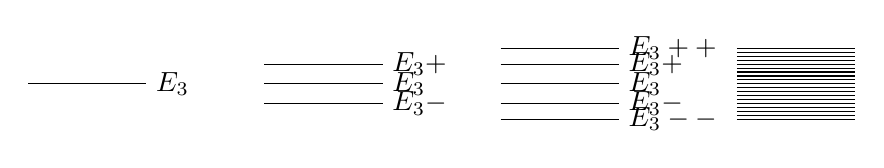
\begin{tikzpicture}
        \draw[] (0,0)--++ (1.5,0) node[right]{$E_3$};
        %
        \draw[] (3,0.25)--++ (1.5,0) node[right]{$E_3+$};
        \draw[] (3,0)--++ (1.5,0) node[right]{$E_3$};
        \draw[] (3,-0.25)--++ (1.5,0) node[right]{$E_3-$};
        %
        \draw[] (6,0.45)--++ (1.5,0) node[right]{$E_3++$};
        \draw[] (6,0.25)--++ (1.5,0) node[right]{$E_3+$};
        \draw[] (6,0)--++ (1.5,0) node[right]{$E_3$};
        \draw[] (6,-0.25)--++ (1.5,0) node[right]{$E_3-$};
        \draw[] (6,-0.45)--++ (1.5,0) node[right]{$E_3--$};
        %
        \draw[] (9,0.45)--++ (1.5,0);
        \draw[] (9,0.40)--++ (1.5,0);
        \draw[] (9,0.35)--++ (1.5,0);
        \draw[] (9,0.30)--++ (1.5,0);
        \draw[] (9,0.25)--++ (1.5,0);
        \draw[] (9,0.20)--++ (1.5,0);
        \draw[] (9,0.15)--++ (1.5,0);
        \draw[] (9,0.1)--++ (1.5,0);
        \draw[] (9,0.05)--++ (1.5,0);
        \draw[] (9,0)--++ (1.5,0);
        \draw[] (9,-0.45)--++ (1.5,0);
        \draw[] (9,-0.40)--++ (1.5,0);
        \draw[] (9,-0.35)--++ (1.5,0);
        \draw[] (9,-0.30)--++ (1.5,0);
        \draw[] (9,-0.25)--++ (1.5,0);
        \draw[] (9,-0.20)--++ (1.5,0);
        \draw[] (9,-0.15)--++ (1.5,0);
        \draw[] (9,-0.1)--++ (1.5,0);
        \draw[] (9,-0.05)--++ (1.5,0);
    \end{tikzpicture}
    \caption{Degenerazione del livello discreto fino a formare una banda}
    \label{fig:Degenerazione del livello discreto fino a formare una banda}
\end{figure}
----------\\
Un elettrone che indice sull abarriera di potenziale ad un'energia inferiore 
1.46\\
%
\cleardoublepage%
la forma d'onda delle funzioni soluzione dell'equazione di shrodinger + di tipo onda piana.\\
\begin{equation}
    \psi(x)= A\cdot \exp{[-jkx]} \text{, con \,\,\, } k=\sqrt{\dfrac{2mE}{h^2}}
\end{equation}
%
\begin{ripasso}[cos'è un onda piana?]
Prima di tutto consiglio di usare 3-D Wave Simulation per "vedere" le onde.\\
     Un'onda piana è caratterizzata da un profilo costante nel tempo, il che significa che \textbf{IL MODULO} dell'ampiezza dell'onda è costante lungo tutto il suo periodo. \\
     %
Un esempio che descrive questa condizione è:
\begin{equation}
    y(t)=A \cdot e^{j(wt+\phi)}
\end{equation}
L'equazione descrive un'onda piana complessa con modulo costante pari ad A. 
%
visivamente:
\begin{center}
    \begin{minipage}{0.49\textwidth}
        \centering
        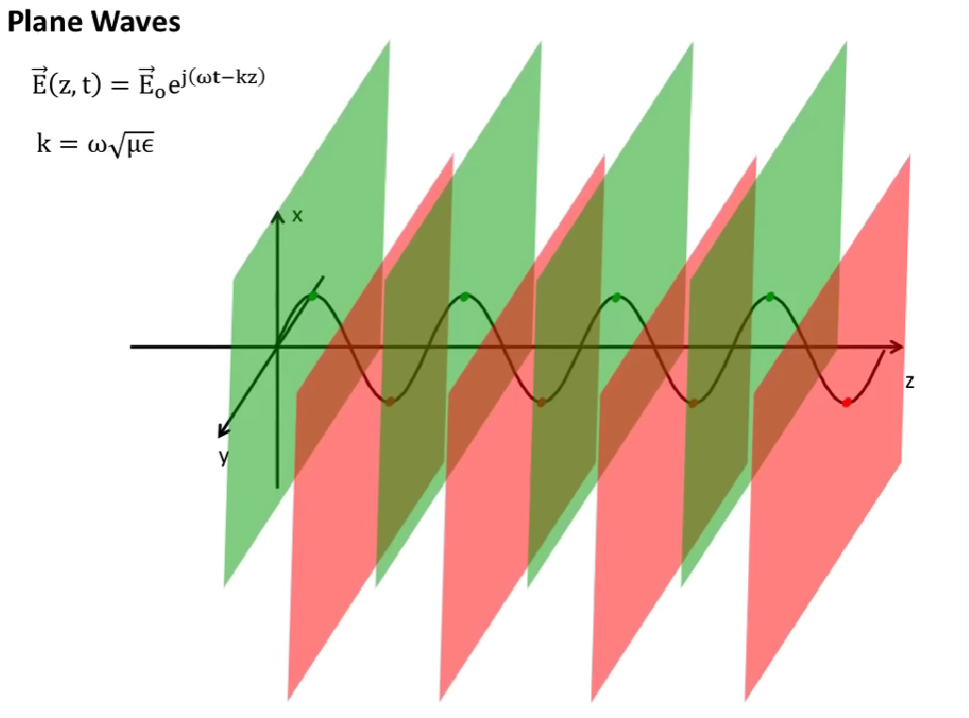
\includegraphics[width=0.85\textwidth]{Immagini_Micro&Nano/Imm_1_Ripasso/rappresentazione di onda piana.png}
        \captionof{figure}{Caption} % Use captionof here
        \label{fig:label1}
    \end{minipage}
    \hfill
    \begin{minipage}{0.49\textwidth}
        \centering
        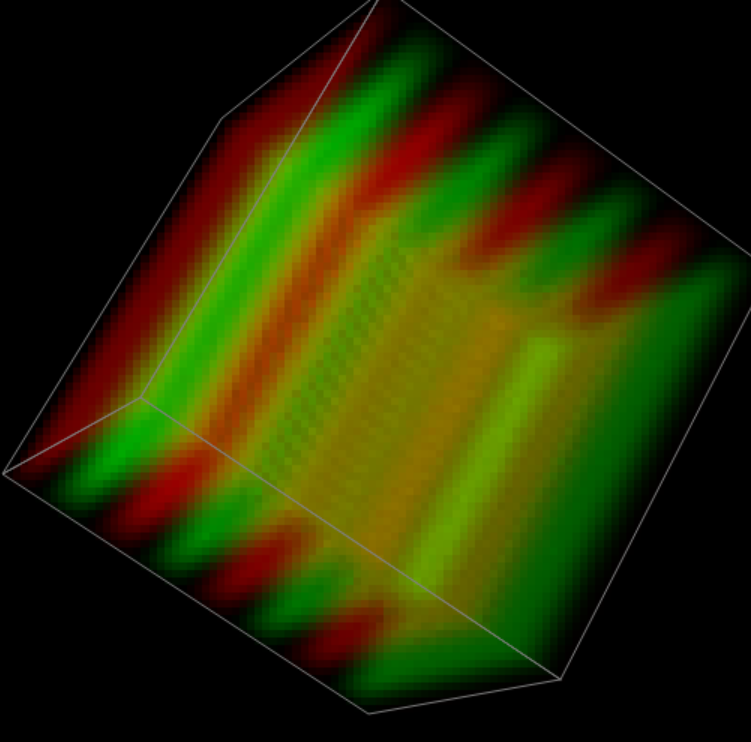
\includegraphics[width=0.65\textwidth]{Immagini_Micro&Nano/Imm_1_Ripasso/rappresentazione 3D onda piana.png}
        \captionof{figure}{Caption} % Use captionof here
        \label{fig:label2}
    \end{minipage}
\end{center}

\end{ripasso}
%
Come descritto nella sezione precedente.
%
\begin{psbox}
%
il pezzo qui sotto è da chiedere a ricevimento. è corretto?
\end{psbox}
Considero una particella in un sistema descritto dalle leggi della meccanica classica (Fisica I), una particella ha un'energia totale E data da:
\begin{equation*}
    E = E_{cinetica}+ E_{potenziale} = K + U
\end{equation*}
Se la particella ha energia totale $E > U_0$  allora si deduce che l'energia cinetica è maggiore di zero, infatti:
\begin{equation*}
    K+U > U \quad =>\quad K>U-U=0
\end{equation*}
La condizione $K>0$ viene intesa (o interpretata) come la capacità dell'elettrone muoversi liberamente sia all'interno (?????ricevimento) che all'esterno della buca di potenziale.\\
La condizione $E < U$ presenta una situazione duale alla precedente: l'elettrone è confinato all'interno della barriera di potenziale.\\
%
In questo contesto la meccanica classica mi aiuta a pensare all'elettrone come un oggetto semplice: sotto cerce condizioni può essere legata alla buca oppure libera da essa (aka: dentro o fuori alla buca).\\
%
Dal punto di vista quantistico la situazione è più complessa poichè la particella è vincolata alla buca, ma esiste comunque la probabilità non nulla che essa si trovi all'esterno della buca.\\
%
la funzione d'onda è ovunque di tipo oscillatorio e supponendo la condizione $E>U_0$, oppure $E \gg U_0$, si trascura l'energia potenziale $U_0$ dall'equazione di Schrodinger:
\begin{equation}
    \dfrac{d^2 \psi(x)}{dx^2} \approx -\dfrac{2mE}{\hslash^2}\psi(x)
\end{equation}
La sua soluzione è:
\begin{equation}
    \psi(x)= \psi^+ \cdot e^{-jkx} + \psi^-\cdot e^{+jkx} \text{, con } k=\sqrt{\dfrac{2mE}{h^2}}
\end{equation}
%
\begin{figure}[htb!]
    \centering
    \begin{tikzpicture}
        %disegno asse x
        \draw[-latex] (-0.5,0)-- (5,0) node[right]{$x$};
        %disegno asse y
        \draw[-latex] (0,-0.5)-- (0,4) node[left]{$U$};
        %disegno barriera di potenziale
        \draw[] (2,0)rectangle++ (1,3) node[pos=.5,align=center]{barriera di \\potenziale};
        %incidente
        \draw[-stealth,decorate,decoration={snake,amplitude=3pt,pre length=2pt,post length=3pt}] (0.5,2.5) -- ++ (1.25,0);
        %trasmessa
        \draw[-stealth,decorate,decoration={snake,amplitude=3pt,pre length=2pt,post length=3pt}] (3.5,1.75) -- ++ (1.25,0);
        %riflessa
        \draw[stealth-,decorate,decoration={snake,amplitude=3pt,pre length=2pt,post length=3pt}] (0.5,1) -- ++ (1.25,0);
    \end{tikzpicture}
    \caption{Caption}%
    \label{fig:enter_label}
\end{figure}
Cioè la funzione d'onda $\psi$ è la somma di due onde piane (una che si propaga verso destra, l'altra verso sinistra); 
inoltre l'energia E può assumere un valore qualsiasi.\\
In presenza di una buca di potenziale, soluzioni dell'equazione di Schròdinger oscillatorie in una regione illimitata dello spazio possono esistere per un insieme centinuo di valori dell'energia (eventualmente appartenente ad un insieme di intervalli); tali soluzioni vengono dette STATI NON LEGATI\\
\\
pg 33 \\
\\
Nel caso di $0<E<U$ l'equazione di shrodinger cambia forma e come risultato si ottiene una funzione d'onda psi a parte reale:
\begin{equation}
    \psi(x)= A\cdot \exp{[-\alpha x]}
\end{equation}
Dove $\alpha=\sqrt{\dfrac{2m(U-E)}{h^2}}$
La funzione d'onda $\psi(x)$ quindi non è più una funzione complessa  e questo è grazie al fatto che k è divento puramente immaginario:
\begin{equation}
    k=\sqrt{\dfrac{2m(E-U)}{h^2}}
\end{equation}
È chiaro che solo per alcuni particolari valori
dell'energia E la funzione d'onda soddisfa alle
condizioni al contorno. In conclusione:
In presenza di una buca di potenziale, soluzioni dell'equazione di
Schrodinger oscillatorie in una regione limitata dello spazio ed evanescenti alirove possono esistere solo per un insieme numerabile di valori dell'energia totale; tali soluzioni vengono dette, stati legati.

questa nuova equazione ci dice che si propaga come onda evanascente (grafico)\\
...\\
1.56
siccome la struttura è periodica, c'è un teorema che dice che $\psi$ è effettivamente un'onda piana però è moltiplicato per un termine che tiene conto della periodicità
\begin{equation}
    \psi(x)=\exp{[-jkx]} \cdot U_k(x)
\end{equation}
Dove $U_k$ è detta funzione d'onda periodica che dipende dalla periodicità degli stati.\\
come si analizza cosa succede all'interno della struttura periodica?\\
grafico\\
Considero zona I e zona II individualmente, come se non fossero pate di un periodo. strutture a parte con le loro equazioni di shrodinger.
la funzione risolta nel primo periodo (Nella zona "I") è:
\begin{equation}
    U_{kI}=A \cdot cos(\beta x) + B \cdot sen(\beta x) \text{, con \,\,\, } \beta=\sqrt{\dfrac{2mE}{h^2}}
\end{equation}
mentre nel secondo periodo (nella zona "II"), l'energia è minore di quella della barriera di potenziale.
Questo allora significa che la funzione non è più periodica perchè deve essere evanescente:
\begin{equation}
    U_{kII}=C \cdot cosh(\alpha x) + D \cdot senh(\alpha x) \text{, con \,\,\, } \beta=\sqrt{\dfrac{2mE}{h^2}}
\end{equation}
%
\\
quindi io ho diviso il mio sistema in 2 pezzi:
 vuoto + barriera con E<U\\
Per trovare la soluzione dell'eq di shrodinger devo raccordare le soluzione dei sottproblemi, cioè impongo le condizioni di contorno.
\begin{enumerate}
    \item $U_{kI}(0) = U_{kII}(0)$
    \item $U_{kI}'(0) = U_{kII}'(0)$
    \item $U_{kI}(a) = U_{kII}(-b)$
    \item $U_{kI}'(a) = U_{kII}'(-b)$
\end{enumerate}
Le condizioni 1) e 2) garantiscono al continuità della funzione e della sua derivata nel punto 0 mentre le condizioni 3) e 4) garantiscono la continuità della funzione e della sua derivata agli astremi.\\
Unendo la prima condizione all'equazione di $U_{kI}$ trovo che
\begin{equation*}
    A=C
\end{equation*}
Dalla seconda condizione al contorno trovo 
\begin{equation*}
    B \cdot \beta = D \cdot \alpha
\end{equation*}
Dalla terza condizione al contorno trovo 
\begin{equation*}
    A \cdot cos(\beta \,a) + B\cdot sen (\beta \,a)= e^{-jkL}\cdot \left[ C \cdot cosh(\alpha \,b)+D \cdot senh(\alpha \,b) \right]
\end{equation*}
Infine, dalla quarta condizione al contorno trovo 
\begin{equation*}
    -A\beta \cdot sen(\beta \,a) + B\beta \cdot sen(\beta \,a)= e^{-jkL}\cdot \left[ C\alpha \cdot senh(\alpha \,b)+D\alpha \cdot cosh(\alpha \,b) \right]
\end{equation*}
Queste equazioni messe insieme formano un sistema lineare omogeneo nelle incognite ABCD
\begin{alignat*}{4}
    A&=B \\
    %
    B &\cdot \beta = D \cdot \alpha \\
    %
    A &\cdot cos(\beta \,a) + B\cdot sen (\beta \,a)= e^{-jkL}\cdot \left[ C \cdot \cosh(\alpha \,b)+D \cdot senh(\alpha \,b) \right] \\
    %
    -A&\beta \cdot sen(\beta \,a) + B\beta \cdot sen(\beta \,a)= e^{-jkL}\cdot \left[ C\alpha \cdot senh(\alpha \,b)+D\alpha \cdot cosh(\alpha \,b) \right]
\end{alignat*}
%
\\
Ma a me non interessa il valore di queste quattro incognite, tuttavia voglio scartare la soluzione banale del sistema che si ottiene nella condizione di termini tutti nulli.\\
matrice e cose\\
ponendo il determinante della matrice diverso da zero significa imporre che il vettore $[A B C B] \neq 0$ e questo ci permette di trovare i livelli di energia ammessi.\\
Il determinante di questa matrice assume forma:
\begin{equation}
    \dfrac{\alpha^2-\beta^2}{2\,\alpha \beta}\cdot senh(\alpha \,a)+cosh(\alpha \,b)+senh(\beta \,a)=cosh(k \,L)
\end{equation}
Quest'equazione è ancora complicata, allora faccio un'altra ipotesi\\
\textbf{HP:}immaginiamo una barriera infinitamente alta e infinitamente sottile: $U_0 \rightarrow \inf $, $b \rightarrow 0$.
Si perviene, quindi, ad una forma dell'equazione più semplice:
\begin{equation}
    F(\beta a)=\underbrace{\dfrac{P}{\beta \, a}\cdot sen(\beta \,a)+cos(\beta \,a)}_{\text{non è detto che sia} -1<\cdot<1} = \underbrace{cos(ka)}_{-1<\cdot<1}
\end{equation}
dove $\beta$ contiene l'energia.
Solo quando "$\beta \cdot a$" è sufficientemente grande il primo termine è compreso tra -1 ed 1 e quindi c'è soluzione, altrimenti per certi valori può succere che non esiste un corrispondente valore di k reale.\\
 ma siccome k (che è una costante di propagazione) è proporzionale alla quantità di moto (hk=p)
e soprattuto dentro beta c'è energia, vuoldire che quel valore di k e di energia non sono compatibili con la soluzione del nostr problema.
questo si traduce nella seguente situazione:
%
\begin{figure}[hbt!]
    \centering
    \begin{tikzpicture}[scale=1]
      % Axes
      \draw[->] (0.5,0) -- (10,0) node[right] {$\beta a$};
      \draw[->] (0.5,-2.5) -- (0.5,2.5) node[above] {$F(\beta a)$};
    
      % Sinusoidal graph with amplitude and frequency inversely proportional to x
      \draw[blue, thick, domain=0.5:9, samples=200, smooth] plot (\x, {20*cos(30*\x^2)/(\x+10))});
      %tratteggi
      \draw[densely dashed] (0.5,1.05)--++ (9,0);
      \draw[densely dashed] (0.5,-1.05)--++ (9,0);
      %sezioni rettangolari
      \draw[ pattern=north west lines, pattern color=gray] (1.345,-1.05) rectangle (2.06,1.05);
      \draw[ pattern=north west lines, pattern color=gray] (2.75,-1.05) rectangle (3.23,1.05);
      \draw[ pattern=north west lines, pattern color=gray] (3.68,-1.05) rectangle (4.06,1.05);
      \draw[ pattern=north west lines, pattern color=gray] (4.38,-1.05) rectangle (4.78,1.05);
      \draw[ pattern=north west lines, pattern color=gray] (5,-1.05) rectangle (5.35,1.05);
      \draw[ pattern=north west lines, pattern color=gray] (5.59,-1.05) rectangle (5.92,1.05);
      %label
      \node at (0.5,1.05)[left]{+1};
      \node at (0.5,-1.05)[left]{-1};
    \end{tikzpicture}
    \caption{Caption}%
    \label{fig:enter_label}
\end{figure}
\\%
ad un certo punto F(beta) sarà tutta dentro -1 ed 1.
solo allora esisterà un valore di k legato a quel particolare valore di beta e quindi ad un corrispondente valore di energia.\\
Nelle altre zone k è complesso ma allora $\psi$ che moltiplica tutta la funzione d'onda del cristallo diventa evanescente (vàa  0) e quindi nel semiconduttore non ci possono stare elettroni per quelle energie.\\
beta, energia e k sono legate ma \\
dire beta oppure energia è lo stesso ma k è la costante di propagazione nel vuoto (come se elett fosse onda piana), beta è la velocità di propagazione nel cristallo mentre k è la quantità di moto associata a...\\
k è legato alal quantità di moto dell'elettrone.
beta è legato all'energia.

\begin{equation}
    h \cdot k = p
\end{equation}
beta dipende da E
Posso scrivere un andamento che mi lega l'energia E a k\\
GRAFICO\\
\begin{exbox}[NOTA]
    
\end{exbox}

\section*{28/09/2023}
Descrivendo graficamente il legame tra energia e $k\dfrac{a}{\pi}$ (dove k è normalizzato rispetto a $\dfrac{a}{\pi}$), ottengo la seguente figura:
\begin{figure}[hbt!]
    \centering
    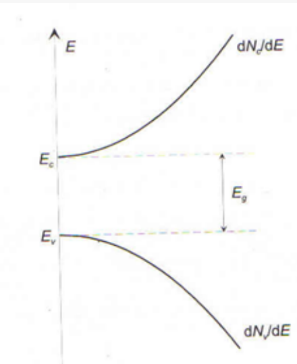
\includegraphics{Immagini_Micro&Nano/Imm_2_Fisica_dei_semiconduttori/densità di stati.PNG}
    \caption{Caption}%
    \label{fig:enter_label}
\end{figure}
%
\begin{figure}[hbt!]
    \centering
    \begin{tikzpicture}
        %disegno asse x
        \draw[->] (-3.5,0)-- (3.5,0) node[right] {$k\dfrac{a}{\pi}$};
        %disegno asse y
        \draw[->] (0, -0.5) -- (0, 4) node[above] {$\mathcal{E}(k)$};
        %disegno grafico
        \draw[scale=0.5, domain=-4.5:4.5, smooth, variable=\x, red]  plot ({\x},{-0.1*\x*\x + 3} );
        \draw[scale=0.5, domain=-4.5:4.5, smooth, variable=\x, red]  plot ({\x},{0.1*\x*\x + 5} );
        %disegno tratteggi verticali
        \draw[densely dotted] (-2.25,0) node[below]{$-1$}--++ (0,4);
        \draw[densely dotted] (2.25,0) node[below]{$+1$}--++ (0,4);
        %disegno tratteggi orizzontali
        \draw[densely dashed] (-3,0.5)--++ (6,0);
        \draw[densely dashed] (-3,1.5)--++ (6,0);
        %labels
        \node at (-0.01,3.5) [align=center]{banda di \\ conduzione};
        \node at (-0.01,0.5) [align=center]{banda di \\ valenza};
    \end{tikzpicture}
    \caption{Grafico di dispersione}
    \label{fig:Grafico di dispersione}
\end{figure}\\
%
Nei precedenti paragrafi ho detto che all'interno di un SC gli elettroni possiedono dell'energia e quindi hanno uno stato energetico.
%
\begin{psbox}[se l'elettrone ha energia ZERO?]
"Se l'elettrone ha energia nulla significa che non si muove, ma questa particolare condizione non esiste in meccanica quantistica poichè in questo ambito si considera che ogni particella abbia sempre dell'energia, per quanto piccola possa essere".\\
Gli elettroni quindi possono avere proprietà cinematiche a cui si associa un valore di energia e di quantità di moto.\\
%
\textbf{In realtà questa spiegazione è un riassunto inaccurato del principio di indeterminazione di Heisenberg}.\\
Il principio di indeterminazione afferma che è impossibile conoscere contemporaneamente e con precisione la posizione e la quantità di moto di una particella e quindi non è possibile assegnare con precisione un valore esatto all'energia della una particella in un dato istante di tempo.\\
Quindi negli elettroni, in realtà, ci sarà sempre una certa quantità di incertezza associata all'energia e quindi non possiamo mai dire che abbiamo energia nulla. 
\end{psbox}
%
Bisogna però fare una differenza tra cinematica classica e cinematica nei semiconduttori:\\
Nella meccanica classica l'energia cinetica e la quantità di moto di un corpo con massa $m$ sono legate l'una all'altra, da cui si trova che l'energia ha un andamento di tipo quadratico.
%
\begin{figure}[hbt!]
    \centering
    \begin{tikzpicture}[scale=0.9,transform shape]
        \filldraw[fill=black, thick] (0,0) circle (0.05) node[right]{$m$};
        \draw[-latex] (0.6,0.05)-- (1.5,0.75) node[right]{$E_c=\dfrac{1}{2}m\underline{v}^2$};
        \draw[-latex] (0.6,-0.05)-- (1.5,-0.75) node[right]{$\underline{p}=m \, \underline{v}$};
        \node at (3.5,0)[right]{$\Rightarrow \, E_c=\dfrac{\underline{p}^2}{2m} $};
    \end{tikzpicture}
\end{figure}\\

%
Gli elettroni nei semiconduttori invece, presentano una relazione tra energia e vettore k (contenuta all'interno della funzione $\psi$), quest'ultimo contenuto anche nella quantità di moto di un elettrone $p=\hslash k$. trovare le equazione corrette nella figura
\begin{figure}[hbt!]
    \centering
    \begin{tikzpicture}[scale=0.9,transform shape]
        \filldraw[fill=black, thick] (0,0) circle (0.05) node[right]{$m$};
        \draw[-latex] (0.6,0.05)-- (1.5,0.75) node[right]{$E_c=\dfrac{1}{2}m\underline{v}^2$};
        \draw[-latex] (0.6,-0.05)-- (1.5,-0.75) node[right]{$\underline{p}=\hslash \, k$};
    \end{tikzpicture}
\end{figure}\\

 Tale relazione và a costruire la figura iniziale, chiamata diagramma di dispesione e rappresenta la relazione dell'energia in funzione di k.\\
 ------------------------------\\
La sua natura corpuscolare viene meno in favore della natura ondulatoria da quis i ha il diagramma di dispersione.??????\\
 ------------------------------\\
In pratica, dentro il semiconduttore, io non posso più considerare energia e quantità di moto legate come se fossi nella meccanica classica ed inoltre io sò che gli elettroni esistono in delle fasce di energia ammissibili. \\
min9.09\\
l'andamento è mostrato in figura ??\\
Perciò, in un primo momento, penserei di fare un miscuglio di formule analitiche, ovvero di considerare la legge della cinematica classica e buttarci dentro il valore della quantità di moto della particella ($\underline{p}$) che fa parte "del mondo quantistico", ottenendo:

\begin{equation}
    E_c=\dfrac{p^2}{2m}=\dfrac{\hslash^2k^2}{2m}
\end{equation}

Ma nel caso quantistico non c'è un legame tra E e k di tipo quadratico poichè il diagramma di dipersione mostra un andamento non quadratico e quindi l'equazione precedente poichè non descrive correttamente tutto l'andamento.\\
Tuttavia posso fare l'approssimazione di $k$ sufficientemente piccolo ($k \approx 0$) in modo da semplificare l'andamento del diagramma di dispersione come fosse di tipo parabolico e quindi rendere valida l'equazione:
\begin{equation}
    E=\dfrac{\hslash^2 k^2}{2m}
\end{equation}
\textbf{Devo tenere in considerazione che $k$ piccolo è sinonimo di quantità di moto ed energia basse}.
Tale approssimazione è mostrata in figura:
\begin{figure}[hbt!]
    \centering
    \begin{tikzpicture}
        %disegno asse x
        \draw[->] (-3.5,0)-- (3.5,0) node[right] {$k$};
        %disegno asse y
        \draw[->] (0, -0.5) -- (0, 4) node[above] {$\mathcal{E}$};
        %disegno grafici rossi
        \draw[scale=0.5, domain=-4.5:4.5, smooth, variable=\x, red]  plot ({\x},{-0.1*\x*\x + 3} );
        \draw[scale=0.5, domain=-4.5:4.5, smooth, variable=\x, red]  plot ({\x},{0.1*\x*\x + 5} );
        %disegno grafici verdi
        \draw[scale=0.5, domain=-1.65:1.65, smooth, variable=\x, green!50!black]  plot ({\x},{-0.75*\x*\x + 3} );
        \draw[scale=0.5, domain=-1.65:1.65, smooth, variable=\x, green!50!black]  plot ({\x},{0.75*\x*\x + 5} );
        %disegno tratteggi verticali
        \draw[densely dotted] (-2.25,0) node[below]{$-1$}--++ (0,4);
        \draw[densely dotted] (2.25,0) node[below]{$+1$}--++ (0,4);
        %disegno tratteggi orizzontali
        \draw[densely dashed] (-3,0.5)--++ (6,0);
        \draw[densely dashed] (-3,1.5)--++ (6,0);
    \end{tikzpicture}
    \caption{Grafico di dispersione vero(rosso) ed approssimato(verde)}
    \label{fig:Grafico di dispersione vero ed approssimato}
\end{figure}\\
%
quindi $E=\dfrac{\hslash^2 k^2}{2m}$ è l'equazione che si avrebbe nello spazio libero ma non dentro al SC, se non per k piccoli.
Questo implica che su ogni banda, l'energia in funzione di k è data dalla somma dell'energia in $k=0$ + un "termine correttivo" che serve per descrivere l'andamento vero dell'energia quando k non è piccolo:
\begin{equation}
    \left. E(k)\right |_{k\rightarrow 0} \approx  \underbrace{\underbrace{E(k=0)}_{\text{andamento approssimato}} + \, \, \dfrac{\hslash k^2}{2m^*}}_{\text{andamento reale}}
\end{equation}
$m^*$ è chiamata massa efficace ed ha la dimensione di una massa. Questo parametro è l'elemento chiave nell'equazione perchè dovrò sceglierlo in maniera opportuna in modo che la somma totale mi rappresenti il vero diagramma (con ammessi piccoli errori) in un range tale per cui k è piccolo.
\begin{psbox}
    Un processo simile ( ma assolutamente non uguale) l'ho studiato a campi elettromagnetici con la teoria di Sommerfield. l'antenna in presenza di terreno può essere studiata come antenna in presenza di piano PEC (ideale) + un termine correttivo che tende a 0 per $\sigma \rightarrow \inf$.\\

    Questo non ha nulla a che fare con quanto detto ma è giusto per similitudine:\\
    \[E = E_{ideale}+E_{correttivo}\]
    dove $E_{correttivo}$ è il termine correttivo che tente a 0 per $k \rightarrow 0$.\\
    Se ci pensi il valore ideale sarebbe l'equazione della meccanica classica:)
\end{psbox}
La massa efficace è un numero il cui valore dipende dalla banda in cui si trova l'elettrone (dipende cioè dall'energia della particella) e quindi, per ottenere un corretto andamendo del grafico di dispersion,  dovrò associare all'elettrone in banda di conduzione la massa $m_n^*+$ e dòvrò associare all'elettrone in banda di valenza la massa $m_n^*-$. \\
C'è però una piccola osservazione da fare. in banda di valenza l'energia è data dal movimento delle lacune, ovvero "alla mancanza dell' elettrone" e quindi è a queste lacune che io associerò la massa in banda di valenza: $m_h^*-$ .\\

E' importante ricordare che questa massa non ha nulla a che fare con la vera massa degli elettroni e delle lacune in quanto è uno stratagemma matematico che noi abbiamo adottato per approssimare il diagramma di dispersione con la forma tipica dell'energia nello spazio libero.
\begin{figure}
    \centering
    \begin{tikzpicture}
        %disegno asse x
        \draw[->] (-0.5,0)-- (3.5,0) node[right] {$k$};
        %disegno asse y
        \draw[->] (0, -0.5) -- (0, 4) node[above] {$\mathcal{E}$};
        %disegno grafici verdi
        \draw[scale=0.5, domain=-1.65:1.65, smooth, variable=\x, green!50!black]  plot ({\x+2.5},{-0.75*\x*\x + 3} );
        \draw[scale=0.5, domain=-1.65:1.65, smooth, variable=\x, green!50!black]  plot ({\x+2.5},{0.75*\x*\x + 5} );
        %label
        \node at (1.4,3.5)[]{$m_n^*+$};
        \node at (1.4,0.5)[]{$m_h^*-$};
    \end{tikzpicture}
    \caption{Caption}%
    \label{fig:enter_label}
\end{figure}
-\\
Non solo le masse efficaci dovranno avere valori opportuni (sicuramente diversi tra loro) ma dovranno avere anche segno opposto. Infatti, osservando il diagramma di distribuzione, si  vede che una parabola è rivolta vero l'altro e l'altra è rivolta verso il basso e pertanto sceglierò $m_n^*+ >0$ per gli elettroni in banda di conduzione e $m_h^*-<0$ per quelle in banda di valenza.\\
Il segno delle masse efficaci quindi dipende dal fatto che si stia considerando banda di conduzione o di valenza ma il loro modulo è inversamente proporzionale alla curvatura del campo elettrico del diagramma di dispersione.\\
Se la curvatura è maggiore allora avrò bisogno di una massa efficace minore e viceversa.
riassumento:
\begin{itemize}
    \item in BC avrò una $m_n^* >0$
    \item in BV avrò una $m_h^* <0$
\end{itemize}
\begin{tikzpicture}[overlay]
    \node at (5.5,1.15)[right]{con};
    \node at (6.5,1.55)[right]{$|m_n|$};
    \node at (6.5,0.75)[right]{$|m_h|$};
    \node at (7.5,1.15)[right]{$1/\alpha \,\, \dfrac{d^2E(k)}{dk^2}$};
\end{tikzpicture}
Quello che si scopre nella pratica è che 
\begin{equation}
    \left | m_n^* \right | < \left | m_h^* \right | 
\end{equation}
Da questo si deduce che le lacune sono più pesanti degli elettroni e si porterà le sue relative implicazioni a seconda dei portatori che creano la corrente:
minore è il valore della massa efficace e più veloce sarà la corrente, per queto dispositivi che sfruttano al corrente di elettroni sono migliori.

\subsection{Semplificazione della massa: Il vantaggio di introdurre la massa efficace }
L'elettrone si muove all'interno di un semiconduttore soggetto all'energia potenziale di buche di potenziale periodiche. Dato però che l'energia totale E dipende dalla somma di U e di K, si ha che calcolare l'energia E risulta complesso poichè il potenziale non è costante.\\
Innanzitutto considero che il diagramma di $E(k)$ senza appossimazioni vale per un profilo periodico delle buche come in questa figura:
gli elettroni possono stare in banda di conduzione o valenza ma hanno la loro massa m vera.
-----------------\\
il diagramma di radiazione vero (rosso) fà riferimento al caso di solido cristallino con bande periodiche.  

\begin{figure}[htb!]
    \centering
    \begin{tikzpicture}[scale=0.75, transform shape]
        %disegno asse x
        \draw[-latex] (-0.5,0)-- (11,0) node[right]{$x$};
        %disegno asse y
        \draw[-latex] (0,-4)-- (0,1) node[left]{$U$};
        %disegno buche
        \draw[very thick,black] (0,0)--++ (1,0)--++ (0,-4);
        \draw[very thick,black] (2.5,-4)--++ (0,1)--++ (1,0)--++ (0,-1);
        \draw[very thick,black] (5,-4)--++ (0,1)--++ (1,0)--++ (0,-1);
        \draw[very thick,black] (7.5,-4)--++ (0,1)--++ (1,0)--++ (0,-1);
        \draw[very thick,black] (10,-4)--++ (0,4)--++ (1,0);
        %disegno i nuclei 
        \node[circle,fill=black,inner sep=0pt,minimum size=6pt,label=nucleo 1] at (1.75,0) {};
        \node[circle,fill=black,inner sep=0pt,minimum size=6pt,label=nucleo 2] at (4.25,0) {};
        \node[circle,fill=black,inner sep=0pt,minimum size=6pt,label=nucleo 3] at (6.75,0) {};
        \node[circle,fill=black,inner sep=0pt,minimum size=6pt,label=nucleo 4] at (9.25,0) {};
        %disegno bande
        \draw[pattern=north west lines, pattern color=cyan!50!blue] (1,0) rectangle (10,-0.5);
        \draw[ pattern=north west lines, pattern color=blue] (1,-3.25) rectangle (2.5,-3.75);
        \draw[ pattern=north west lines, pattern color=blue] (3.5,-3.25) rectangle (5,-3.75);
        \draw[ pattern=north west lines, pattern color=blue] (6,-3.25) rectangle (7.5,-3.75);
        \draw[ pattern=north west lines, pattern color=blue] (8.5,-3.25) rectangle (10,-3.75);
        %label bande
        \draw[latex-] (10.25,-0.5)--++ (1,0) node[align=center,right]{Banda di \\ conduzione};
        \draw[latex-] (10.25,-3)--++ (1,0) node[align=center,right]{Banda di \\ valenza};
        %per centrare la figura ricrei i label delle bande a sinistra ma li faccio invisibili
        \draw[latex-,white] (-0.25,-0.5)--++ (-1,0) node[align=center,left]{Banda di \\ conduzione};
        \draw[latex-,white] (-0.25,-3)--++ (-1,0) node[align=center,left]{Banda di \\ valenza};
    \end{tikzpicture}
    \caption{Caption}%
    \label{fig:enter_label}
\end{figure}
%
in particolare esisteranno delle bande di valenza (all'interno delle quali l'elettrone si muove con la sua massa m vera) e delle bande di conduzione.\\
%
Se introduco la massa efficace posso  vedere il sistema costituito dalle buche di potenziale periodiche in maniera semplificata come se fosse nello pazio libero, valido solo per k piccole. quello che ottengo alla fine è un qualcosa che assomiglia molto ad una sola buca di potenziale a lunghezza L ed a pareti infinite:
%
\begin{figure}[htb!]
    \centering
    \begin{tikzpicture}[scale=0.75, transform shape]
        %disegno asse x
        \draw[-latex] (-0.5,0)-- (11,0) node[right]{$x$};
        %disegno asse y
        \draw[-latex] (0,-4)-- (0,1) node[left]{$U$};
        %disegno buche
        \draw[very thick,red] (0,0)--++ (1,0)--++ (0,-4)--++ (9,0)--++ (0,4)--++ (1,0);
        %disegno i nuclei 
        \node[circle,fill=black,inner sep=0pt,minimum size=6pt,label=nucleo 1] at (1.75,0) {};
        \node[circle,fill=black,inner sep=0pt,minimum size=6pt,label=nucleo 2] at (4.25,0) {};
        \node[circle,fill=black,inner sep=0pt,minimum size=6pt,label=nucleo 3] at (6.75,0) {};
        \node[circle,fill=black,inner sep=0pt,minimum size=6pt,label=nucleo 4] at (9.25,0) {};
        %disegno bande
        \draw[pattern=north west lines, pattern color=cyan!50!blue] (1,0) rectangle (10,-0.5);
        \draw[ pattern=north west lines, pattern color=blue] (1,-3.25) rectangle (10,-3.75);
        
        %label bande
        \draw[latex-] (10.25,-0.5)--++ (1,0) node[align=center,right]{Banda di \\ conduzione};
        \draw[latex-] (10.25,-3)--++ (1,0) node[align=center,right]{Banda di \\ valenza};
        %per centrare la figura ricrei i label delle bande a sinistra ma li faccio invisibili
        \draw[latex-,white] (-0.25,-0.5)--++ (-1,0) node[align=center,left]{Banda di \\ conduzione};
        \draw[latex-,white] (-0.25,-3)--++ (-1,0) node[align=center,left]{Banda di \\ valenza};
    \end{tikzpicture}
    \caption{Caption}%
    \label{fig:enter_label}
\end{figure}
%
gli estremi del semiconduttore rimangono invariati. La banda di valenza e conduzione che si distribuiscono in tutto il semiconduttore con elettroni che si muovono con massa efficace di opportuno valore.\\
%
Alla fine ho ottenuto un metodo che mi permette di studiare la statistica degli elettroni all'interno del semiconduttore e sono in grado di farlo perchè uso il SC come se fosse lo spazio libero $U(x) = cost$ ma, con la sola differenza che l'energia E non è continua ma rimane ancora discretizzata perchè ovviamente non siamo nel vero caso di mezzo vuoto.\\
%
\cleardoublepage%
\subsection{Densità di stati}
La densità di stati è il numero di stati disponibili per unità di volume ed energia.\\
La quantità di moto degli elettroni nel semiconduttore, approssimato come spazio libero vale:
\begin{equation}
    p=\hslash k = \sqrt{2m^*E}
\end{equation}
Ipotizzando quindi che il semiconduttore si comporti come una buca di potenziale lunga L, si avrà che i livelli energetici consentiti sono:
\begin{equation}
    E_n=\dfrac{n^2\ \hslash \ \pi^2}{2\ m^* \ L^2}
\end{equation}
Sostituendo si ha:
\begin{equation}
    p=\dfrac{n\ h}{2\ L}
\end{equation}
Ora faccio dei ragionamenti geometrici ma anche astratti:\\
Si consideri uno spazio tridimensionale, per cui la quantità di moto degli elettroni sarà composta da una combinazione di tre termini ($\overline{p}(x,y,z)$) con indice n variabile nelle tre dimensioni($ n_x, n_y, n_z$).\\
Il volume occupato da ogni stato elettronico nello spazio delle quantità di moto sarà:
%
\begin{equation}
    \left( \dfrac{h}{2L}\right)^3 \cdot \dfrac{1}{2}
\end{equation}
%
con $\left( \dfrac{h}{2L}\right)^3$ che rappresenta il volume del singolo stato e il diviso due è dovuto al fatto che lo spazio è suddiviso per le due particelle di spin opposto che possono occupare tale stato.\\
%
Il volume nello spazio delle quantità di moto ha una andamento sferico, per cui per un incremento di dp si avrà un incremento di volume di:
\begin{equation}
    \dfrac{4\pi p^2\ dp}{2^3}
\end{equation}
%
Si stanno considerando gli elettroni in banda di conduzione per cui si può riprtare la quantità di moto rispetto ad Ec:
%
\begin{equation}
    p=\sqrt{2\ m_n^* \,(E-E_c)}
\end{equation}
%
moltiplicando per dp si può trovare che
%
\begin{align}
    p\ dp & =\sqrt{2\ m_n^*(E-E_c)}\ dp \nonumber \\
    p\ dp & =\sqrt{2\ m_n^*(E-E_c)}\ d\left(\sqrt{2\ m_n^*(E-E_c)}\right) \nonumber\\
    p\,dp &= m_n^* dE
\end{align}
%
Se si realizza il rapporto tra i due volumi si trovano il numero di stati disponibili al variare di p:\\
%
\noindent\begin{minipage}{0.5\textwidth}
    %
\begin{equation}
    dN_c(p)=\dfrac{\dfrac{4\ \pi\ p^2 dp}{8}}{\left( \frac{h}{2L}\right)^3 \cdot \dfrac{1}{2}} = \dfrac{8\ \pi\ L^3\ p^2\ dp}{h^3}
\end{equation}
%
Sostituendo $pdp=m_n^*dE$ e $p=\sqrt{2\ m_n^*(E-E_c)}$ \\nell'espressione superiore e considerando $L=1$, si trova:
%
\begin{equation}
    dN_c=\dfrac{4\ \pi
    }{h^3}(2m_n^*)^{\dfrac{3}{2}}\sqrt{E-E_c} \,dE
\end{equation}
%
Analogamente si può trovare per le lacune in valenza:
%
\begin{equation}
    dN_v=\dfrac{4\ \pi
    }{h^3}(2m_h^*)^{\dfrac{3}{2}}\sqrt{E_v-E} \,dE
\end{equation}
%
\end{minipage}
\hfill%
\begin{minipage}{0.4\textwidth}\raggedleft
    \begin{center}
        \begin{tikzpicture}[scale=0.56]
            %disegno l'asse y
            \draw[-latex] (0,-4.5) -- (0,4.5) node[anchor=south east] {$E$};
            %disegno le condentrazioni n e p
            \draw(0,1) node[left,thick]{$E_C$} arc (270:360:3) node[left]{$\dfrac{dN_c}{dE}$};
            \draw(0,-1) node[left,thick]{$E_V$} arc (90:0:3) node[left]{$\dfrac{dN_v}{dE}$};
            % tratteggi
            \draw[densely dashed] (0,1)--++ (5,0);
            \draw[densely dashed] (0,-1)--++ (5,0);
            \draw[latex-latex] (4.5,-1)--++ (0,2);
            \draw[densely dashed] (0,0) node[left]{$E_F$}--++ (4,0);
            \node at (4.5,0)[right]{$E_g$};
        \end{tikzpicture}
        \captionof{figure}{Andamento della densità di stati degli elettroni in BC e delle lacune in BV}
  \end{center}
\end{minipage}
\subsection{Distribuzione di Fermi-Dirac}
%
Tra i due livelli $E_v$ ed $E_c$ si posiziona un livello $E_F$ detto energia di fermi.\\
In generale il livello di Fermi non è noto a priori ma possiamo dire che rappresenta il livello al di sotto del quale, in condizioni di temperatura a 0 Kelvin ed in equilibrio termodinamico, tutti i livelli energetici sono occupati da elettroni mentre quelli sopra sono vuoti.\\
La densita in energia di un insieme di elettroni e lacune in equilibrio termodinamico si esprime come il prodotto di due
fattori: \textbf{la densità degli stati} (che rappresenta il numero di stati disponibili per unità di volume all'energia E) \textbf{e la funzione distribuzione} (che rappresenta la probabilita di occupazione di uno stato a energia E).\\
Anche se gli stati in un sistema quantizzato di dimensioni finite sono quantità discrete e numerabili, comunque il numero degli stati per unita di volume è cosi grande da consentire un trattamento come se fosse continuo. \\
Consideriamo il numero di stati dN di energia compresa fra
$E$ ed $E+dE$. questo é dato da: \\
%
 eq pg 64
 %
 \\
La funzione di distribuzione di Fermi-Dirac descrive la probabilità che un livello energetico E sia occupato da elettroni:
%
\begin{equation}
    f_{FD}(E)=\dfrac{1}{1+e^{\left(\dfrac{E-E_F}{k_B T}\right)}}
\end{equation}
%
Vediamo, dall'equazione, che la distribuzione di Fermi-Dirac dipende dall'energia e dalla temperatura:
Per T=0K si avrà un gradino,\textbf{indicando che tutti gli stati con energia inferiore al livello di Fermi sono pieni mentre tutti gli stati con energia superiore sono vuoti}. Per temperature seperiori si avrà un andamento esponenziale.\\
La probabilita di occupazione al livello di Fermi é pari a $\dfrac{1}{2}$ a qualsiasi temperatura. Poiché: \\
??????????????????????????
probabilita stato vuoto = 1 — probabilita stato pieno, \\
\begin{exbox}[la distribuzione di Fermi-Dirac per le lacune sara:]
    \begin{equation}
    1-f_{FD}(E)=\dfrac{1}{1+e^{\left(\dfrac{E_F-E}{k_B T}\right)}}
    \end{equation}
    In tale distribuzione complementare (a 0 K) tutti gli stati sono vuoti (di lacune)
    per energie inferiori al livello di Fermi e, tutti gli stati sono pieni per energie superiori
    al livello di Fermi.
\end{exbox} 
%
Se l'energia $E \gg E_F$, si parla di livelli energetici di conduzione. in questo caso la distribuzione di Fermi-Dirac diventa una distribuzione di Boltzman.
%
\begin{exbox}[PS: distribuzione di Boltzman]
    una distribuzione di Boltzmann (chiamata anche distribuzione di Gibbs) è una distribuzione di probabilità che fornisce la probabilità che un sistema si trovi in un determinato stato in funzione dell'energia di quello stato e della temperatura del sistema. La distribuzione è espressa nella forma:
    %
    \begin{equation}
        {\displaystyle p_{i}\propto \exp \left(-{\frac {\varepsilon_{i}}{kT}}\right)}
    \end{equation}
    %
    dove p i è la probabilità che il sistema si trovi nello stato i,$\varepsilon_i$ è l'energia di quello stato e la costante kT è il prodotto della costante di Boltzmann k e della temperatura termodinamica T .\\
    Il termine "sistema" qui ha un significato ampio; può variare da un sistema microscopico (facendo riferimento ad un singolo atomo o ad un "numero sufficiente" di atomi) a un sistema macroscopico come un serbatoio di stoccaggio del gas naturale.\\
     La distribuzione mostra che gli stati con energia più bassa avranno sempre una maggiore probabilità di essere occupati.
\end{exbox}
%
La condizione $E > E_F$ implica che l'esponenziale nella formula di $f_{FD}(E)$ sia molto più grande di 1, permettedomi di approssimare:
%
\begin{equation}
    f_{FD}(E) \approx \dfrac{1}{e^{\left(\dfrac{E-E_F}{k_B T}\right)}} = e^{\left(-\dfrac{E-E_F}{k_B T}\right)}
\end{equation}
%
Adesso sono in grado di calcolare la densità di di energia degli elettroni nella banda di conduzione n tenendo presente che il numero di elettroni dn presenti nell'intervallo da $E$ a $E+dE$ (cioé la funzione densita in energia) é pari alla densita degli stati disponibili ($dN_c$)
moltiplicata per la probabilita di occupazione $f_{FD}(E)$, cioé: 
%
\begin{equation}
    dn(E) = f_{FD}(E)\cdot dN_c
\end{equation}
%
La densita totale n si ottiene, in funzione di $E_F$, integrando $dn(E)$ su tutte le energie della banda-di-conduzione (cioé da $E_c$ all'energia del vuoto $U_0$): tuttavia-a-causa-del-comportamento esponenziale decrescente per alte energie di $f_{FD}(E)$, si può porre il limite di integrazione superiore a $+ \inf $.
\\
In parole povere, dico che n è dato dall'integrazione del prodotto tra la funzione che indica i posti disponibili e quella che indica la probabilità di occupazione.\\
%
\begin{equation}
    n=\int_{E_c}^{\inf}dN_c(E) \cdot f_{FD}(E)
\end{equation}
%
Si ottiene, nella condizione $E < E_F$ (e quindi con distribuzione di Boltzman), che la densità totale $n$ vale circa:
%
\begin{equation}
    n \approx N_c \cdot e^{\dfrac{E_F-E_C}{k_B T}}
\end{equation}
%
con $N_c=2\dfrac{{(2\pi m_n^* k_B T)}^{\dfrac{2}{3}}}{h^3} \,$ detta densità equivalente di stati in banda di conduzione.\\
$n$ rappresenta il numero di elettroni per unità di volume in banda di conduzione ed osservando la formula vedo che è dipendente dalla temperatura.\\

Il ragionamento è analogo per quanto riguarda le lacune in banda di valenza:
\begin{equation}
    p=\int_{-\inf}^{E_v}dN_v(E) \cdot [1-f_{FD}(E)]
\end{equation}
da cui 
\begin{equation}
    p \approx N_v \cdot e^{\dfrac{E_v-E_F}{k_B T}}
\end{equation}
con $N_v = 2 \dfrac{{(2\pi m_h^* k_B T)}^{\frac{2}{3}}}{h^3}$ chiamata densità equivalente di stati in banda di valenza.\\
Per le lacune la probabilità di occupazione sarà data da $1-f_{FD}(E)$ riportata sotto:
\begin{figure}[hbt!]
    \centering
    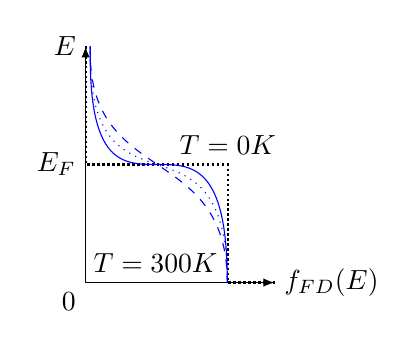
\begin{tikzpicture}[scale=0.6]
        %disegno asse x
        \draw[-latex] (0,0) node[anchor= north east]{$0$}--++ (4,0) node[right]{$f_{FD}(E)$};
        %disegno asse y
        \draw[-latex] (0,0)--++ (0,5) node[left]{$E$};;
        %disegno E
        \draw[thick, densely dotted] (0.01,5)--++ (0,-2.5) node[left]{$E_F$}--++ (3,0) node[anchor=south]{$T=0K$}--++ (0,-2.5) node[anchor=south east]{$T=300K$}--++ (1,0);
        %disegno Ffd
        \draw[blue] (0.1,5)..controls (0.01,0) and (3,5).. (3,0);
        \draw[blue,dotted] (0.1,5)..controls (0.01,1) and (3,4).. (3,0);
        \draw[blue,dashed] (0.1,5)..controls (0.01,2) and (3,3).. (3,0);
        %disegno freccia T
        
    \end{tikzpicture}
    \caption{Caption}%%
    \label{fig:enter_label}
\end{figure}
\begin{figure}[hbt!]
    \centering    
    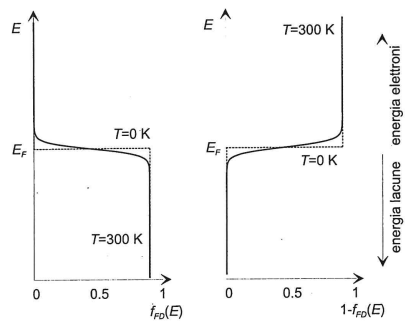
\includegraphics{Immagini_Micro&Nano/Imm_2_Fisica_dei_semiconduttori/fermi dirac.png}
    \caption{Distribuzione di Fermi-Dirac dell'energia degli elettroni e delle lacune}%
    \label{fig:Distribuzione_di_Fermi_Dirac_dell_energia_degli_elettroni_e_delle_lacune}
\end{figure}
\cleardoublepage%%
\begin{figure}
    \centering
    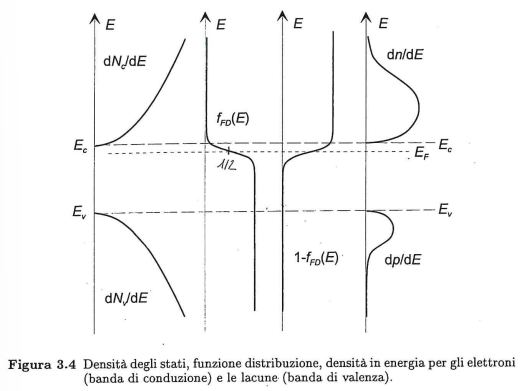
\includegraphics{Immagini_Micro&Nano/Imm_2_Fisica_dei_semiconduttori/stati, distribuzione, energia.png}
    \caption{Densità di stati, funzione di distribuzione, densità di energia per gli elettroni (nella banda di conduzione) e per le lacune (nella banda di valenza) }%
    \label{fig:Densità di stati, funzione di distribuzione, densità di energia per gli elettroni (nella banda di conduzione) e per le lacune (nella banda di valenza)}
\end{figure}
%
\cleardoublepage%%

\section*{02/10/2023}

\begin{center}
    \begin{tikzpicture}    
        %disegno l'asse y
        \draw[thick,->] (0,-4.5) -- (0,4.5) node[anchor=south east] {$E$};
        %disegno le condentrazioni n e p
        \draw(0,1) arc (270:360:3);
        \draw(0,-1) arc (90:0:3);
        %disegno la densità di probabilità
        \draw[blue] (0.1,4)..controls (0,-4) and (4,4).. (4,-4);
        \draw[green] (0.1,-4)..controls (0,4) and (4,-4).. (4,4);
        %
        \draw[blue,pattern=north east lines, pattern color=blue] (0,1)-- (0.2,1) arc (270:370:0.65)..controls (0.55,2.75) and (0.15,2).. (0.15,4)-- (0,4)-- (0,1);
        %
        \draw[red,pattern=north east lines, pattern color=red] (0,-1)-- (0.1,-1) arc (90:0:0.4)..controls (0.5,-1.8) and (0.15,-2).. (0.15,-4)-- (0,-4)-- (0,-1);
    \end{tikzpicture}
\end{center}


Sulla base di queste quantità abbiamo individuato delle densità di stati 

Le abbiamo calcolate come quantità dip dall'energia e inoltre in corrispondenza del livello di fermi di arriva alla probabilità di occupaione di uno di questi stati disponibili
E sull abase del prodotto di queste due quantità, si trovava la quantità idi elettroni che in questo caso rappresenta quella dellla banda di valenza.

Nel caso specifico degli elettroni nella banda in conduzione abbiamo eq n.
Stessa cosa per lacune in banda V
Osserviamo in tutte i due i casi che l'argomento dell'esponenziale è negativo perché ef è minore del minimo della banda C ed è maggiore della banda V.
Se il live fermi per qualche motivo si spostasse verso alto o verso basso, si partirebbe da una situazione in cui le p ed n sono uguali, ad una situazione in cui (es tipo n) la funzione di distribuzione si sposta verso l'alto e quindi la distribuzione n sarà più grande e contemporaneamente una p più piccola = questo è il drogaggio N, per il tipo P succede l'opposto.

Ora dobbiamo vedere risultati che derivano direttamente da queste formule

\subsection{LEGGE DI AZIONE DI MASSA}
Sappiamo che le densità di elettroni e lacune dipendono dal livello di fermi $E_F$ tuttavia
la legge di azione di massa afferma che, in un SC non degenere ed in equilibrio
termodinamico,il prodotto $(p\cdot n)$ non dipende dalla posizione del livello di fermi.Si ha infatti:

\begin{equation}
	p \cdot n=N_C N_V \cdot \exp \left[-\dfrac{E_C-E_V}{k_B T}\right]=
        N_C N_V \cdot \exp \left[-\dfrac{E_G}{k_B T}\right]
\end{equation}

Dove $E_G$ è l'ampiezza della banda proibita del semiconduttore. \\
E' possibile osservare come pn sia inversamente proporzionale all'energy gap pertanto, materiali con $E_G$ grande presentano una minore concentrazione di elettroni in banda di conduzione ( o equivalentemente, una minore concentrazione di lacune in banda di valenza)

\textbf{Il prodotto pn quindi non dipende da $E_F$ \emph{ma solo dalla temperatura e dalle proprietà del semiconduttore}}.\\
Una diretta conseguenza di quanto detto è che il valore del prodotto pn associato ad un generico semiconduttore drogato sarà uguale al prodotto $p_i \cdot n_i$ del semiconduttore intrinseco, portando alla conclusione che il prodotto pn è indipendente dal drogaggio.
\begin{equation}
	p \cdot n=p_i \cdot n_i
\end{equation}
Dove $n_i$ e $p_i$ sono le concentrazioni nel SC intrinseco.
Poiché nel semiconduttore intrinseco elettroni e lacune si generano a coppie $(aka: p_i=n_i)$, la legge di azione di massa può essere riscritta in:
\begin{equation}
	p \cdot n=p_i \cdot n_i=p_i^2=n_i^2
\end{equation}

\begin{center}
    \begin{tikzpicture}
        \begin{axis}[
        xlabel={$\dfrac{1000}{T}$},
        ylabel={$\log(n_i^2) [cm^{-6}]$},
        axis lines=left,
        xmin=0,xmax=5,
        ymin=0,ymax=5,
        ytick={0,2,3.5,4},
        xtick={2,3,4},
        xticklabels={$3$,$4$,$5$},
        yticklabels={$10^0$, $10^8$, $10^{10}$, $10^{16}$},
        unit vector ratio=2 1.1,
        ]
            %retta nera
            \addplot [domain=0.25:3.5,samples=100,color=black,]{-0.5*x+4.1};
            \addlegendentry{$G_e$}
            %retta rossa
            \addplot [domain=0.25: 3,samples=100,color=red,]{-0.7*x+3.6};
            \addlegendentry{$S_i$}
            %retta verde
            \addplot [domain=0.65: 2,samples=100,color=green,]{-1.2*x+3};
            \addlegendentry{$G_eA_S$}
        \end{axis}

    \draw[->,blue] (4,4) node[anchor=south]{$E_G$} ..controls (3,2) and (2,1.5).. (1,1);
    
    \end{tikzpicture}
\end{center}
Riportando su grafico logaritmico la concentrazione di queste quantità in funzione dell'inverso della temperatura, succede che la concentrazione aumenta all'aumentare della temperatura e maggiore è Eg, minore sarà $ni^2$

All'aumentare della temepratura la concentraz di elett auemnta  e viceversa
Siccome gli stati hanno funzione esponenziale e siamo in grafico logaritmico, allora noi vediamo un andamento rettilineo.
L'andamento reale in realtà è approssimato, ottenuto da un'approssimazione del modello ideale.
Per T che aumenta ci sarebbero fenomeni non rettilinei 
%
\subsection{Equazioni di Shockley}
È utile in molti casi esprimere la concentrazioni di elettroni e lacune con riferimento alla concentrazione intrinseca n; e al livello di Fermi intrinseco Epi. In un
semiconduttore non degenere si ha infatti: 
%
\begin{equation}
    n=N_C \cdot \exp{\left( \dfrac{E_F-E_c}{k_B T}\right)}
\end{equation}
%
e per il semiconduttore intrinseco: 
%
\begin{equation}
    n_i=N_C \cdot \exp{\left( \dfrac{E_{Fi}-E_c}{k_B T}\right)}
\end{equation}
%
da cui, dividendo membro a membro: 
%
\begin{equation}
    n=n_i \cdot \exp{\left( \dfrac{E_{F}-E_{Fi}}{k_B T}\right)}
\end{equation}
%
Analogamente:
%
\begin{equation}
    p = p_i \cdot \exp{\left( \dfrac{E_{Fi}-E_{F}}{k_B T}\right)}
\end{equation}
%
Le relazioni precedenti, dette equazioni di Shockley, esprimono il fatto che quando
il livello di Fermi coincide con il valore intrinseco, le concentrazioni di elettroni e
lacune assumono i valori propri del materiale intrinseco $n = n_i$, $p = n_i$. Si noti
che moltiplicando le due equazioni di Shockley si ottiene $pn = n_i^2$ identicamente.
%
\subsection*{DISTRIBUZIONE DI CORRENTE}
Supponiamo di avere due semiconduttori uguali caratterizzati però da una differente posizione del livello energetico di fermi. 
\begin{center}
    \begin{tikzpicture}[scale=0.6]
        %disegno mezzo 1
        \node at (2,2) [anchor=south]{SC1};
        \draw(0,1.5) --++ (4,0);
        \draw(0,-1.5) --++ (4,0);
        \draw[dashed, red] (0,0.75) node[anchor=east]{$E_{F1}$} --++ (4,0); %Ef1
        %disegno mezzo 2
        \node at (9,2) [anchor=south]{SC2};
        \draw(7,1.5) --++ (4,0);
        \draw(7,-1.5) --++ (4,0);
        \draw[dashed, red] (7,-0.75) --++ (4,0) node[anchor=west]{$E_{F2}$}; %Ef2
    \end{tikzpicture}
\end{center}
I due semiconduttori al momento sono separati, distinti l'uno dall'altro ma cosa succede quando si uniscono?
Due o più sistemi in equilibrio termodinamico posti fra loro in contatto, sono caratterizzati dallo stesso livello di fermi. 
Tipicamente viene detto che il livello di fermi si allinea ad un certo valore costante, quindi nel nostro caso:
\begin{equation}
	E_{F1} = E_{F2}
\end{equation}

È tipo il principio dei vasi comunicanti
\newline

Perché succede questo?\\
Consideriamo due materiali semiconduttori identici caratterizzati dalla stessa densità di stati disponibili $(aka: N_{V1}=N_{V2}$ e $ N_{C1}=N_{C2})$.
L'unica cosa diversa tra i due è il livello di Fermi e, di conseguenza, anche la funzione distribuzione di probabilità di Fermi-Dirac (che per definizione è centrata intorno al livello di Fermi) sarà diversa.\\

Quindi avrò a che fare con livelli energetici occupati da elettroni nel SC1 che si affacciano a livelli energetici non occupati nel SC2.
Esisterà quindi la probabilità che una carica passi dal SC 1 al SC 2 e viceversa tuttavia, noi dobbiamo considerare il caso di equilibrio.\\
Succede che quando il sistema è in equilibrio termodinamico, la probabilità di trasferimento della carica dal mezzo 1 al 2 $(aka: P_1 \rightarrow 2)$ dovrà necessariamente essere uguale alla probabilità di trasferimento della carica dal mezzo 2 al 1 $(aka: P_{2 \rightarrow 1})$.

La probabilità $P_{1 \rightarrow 2}$ implica due condizioni:
\begin{enumerate}
    \item che lo stato di energia nel mezzo 1 sia pieno (ovvero c'è un elettrone)
    \item che lo stato di energia nel mezzo 2 sia vuoto (ovvero non ci sono elettroni)
\end{enumerate}
\begin{psbox}
    In termini detti dal libro: la probabilità di trasferimento da 1 a 2 è proporzionale al numero di stati occupati nel mezzo 1 e al numero di stati occupati nel mezzo 2.
\end{psbox}

la probabilità di passare da 1 a 2 è la probabilità congiunta di queste due osservazioni:
\begin{equation}
P_{1 \rightarrow 2} = N_{C1} (E) \cdot f_{FD1} (E) \times N_{C2} (E) \cdot \left[ 1 - f_{FD2}(E) \right] 
\end{equation}

La medesima osservazione si svolge per il passaggio da 2 ad 1:

\begin{equation}
	P_{2 \rightarrow 1} = N_{C2}(E) \cdot f_{FD2}(E) \times N_{C1}(E) \cdot  \left[ 1 - f_{FD1}(E)\right] 
\end{equation}

Dove $\left[1-f_FD (E)\right]$ indica la probabilità che il livello sia vuoto.\\
Quando queste due probabilità sono forzate ad essere identiche (perché siamo all'equilibrio e quindi si parla di trasformazione adiabatica), abbiamo che: 

\begin{equation}
	N_{C1}(E) \cdot f_{FD1}(E) \times N_{C2}(E) \cdot \left[ 1-f_{FD2}(E) \right] = N_{C2}(E) \cdot f_{FD2}(E) \times N_{C1}(E) \cdot \left[ 1-f_{FD1}(E)\right]
\end{equation}

Siccome i semiconduttori sono identici, le densità di stati saranno identiche comportandone la semplificazione dall'equazione:

\begin{equation}
	f_{FD1}(E) \times \left[1-f_{FD2}(E)\right]=f_{FD2}(E) \times \left[1-f_{FD1}(E)\right]
\end{equation}

La funzione di fermi dirac dipende unicamente dalla distanza che c'è tra il livello di energia ed il livello di fermicome mostrato dall'equazione

\begin{equation}
	f_{FD} = \dfrac{1}{1 + \exp \left[\dfrac{E-E_F}{k_B T}\right]}
\end{equation}

L'unica possibilità che abbiamo affinché l'identità sia verificata è che questi prodotti siano uno ad uno uguali fra loro:

\begin{align}
f_{FD1}(E) &= f_{FD2}(E)\\
\left[1-f_{FD2}(E)\right] &= \left[ 1-f_{FD1}(E)\right]
\end{align}


L'unica soluzione che verifica questa uguaglianza è l'allineamento del livello di Fermi per entrambi i mezzi ad un valore uguale e costante.
Nell'intorno del livello di fermi devono comunque essere rispettate le debite distanze tra le bande per cui si avrà un qualcosa come:
\begin{center}
    \begin{tikzpicture}[scale=0.90]
        %disegno l'unione di due SC
        %mezzo 1
        \draw(0,1.5) --++ (4,0);
        \draw(0,-1.5) --++ (4,0);
        %mezzo 2
        \draw(7,3) --++ (4,0);
        \draw(7,0) --++ (4,0);
        %livello di fermi dei mezzi
        \draw[dashed, red] (0,0.75) --++ (11,0) node[anchor=north east]
        {$E_{F1}=E_{F2}$};
        %livello di fermi del SC intrinseco
        \draw[dash dot, black] (0,0) --++ (4,0) (4,0)..controls (5.5,0) and (5.5,1.5).. (7,1.5) --++ (4,0) node[anchor=south east]
        {$E_{Fi}$};
        
        %intersezione
        \draw[] (4,1.5)..controls (5.5,1.5) and (5.5,3).. (7,3);
        \draw[] (4,-1.5)..controls (5.5,-1.5) and (5.5,0).. (7,0);
    
        %delimitazioni
        \draw[densely dotted] (4,-1.9)--++ (0,6.5);
        \draw[densely dotted] (7,-1.9)--++ (0,6.5);
        \node at (5.5,4.7) [align=center]{flessione \\ delle bande};
        \draw[thick, dashed] (4,-1.5)--++ (7,0);
        \draw[thick, dashed] (7,3)--++ (-7,0);
        %concentrazione n
        \draw(2,1.7) --++ (0,2.4);
        \draw(2,1.7)..controls (3.3,2.2) and (2,3.1).. (2,4);
        \draw[pattern=north east lines, pattern color=blue] (2,3)-- (2.34,3)..controls (2.34,3.1) and (2.1,3.3).. (2,4);
        \node at (2.25,2.3)[]{$n$};
        %concentrazione p
        \draw(9,-0.2) --++ (0,-2.4);
        \draw(9,-0.2)..controls (7.7,-0.7) and (9,-1.6).. (9,-2.5);
        \draw[pattern=north east lines, pattern color=Hcolour] (9,-1.5)-- (8.67,-1.5)..controls (8.67,-1.6) and (8.9,-1.8).. (9,-2.5);
        \node at (8.75,-0.85)[]{$p$};
        % metto elettroni
        \draw[blue, arrows={-Triangle[angle=90:6pt,blue,fill=blue]}] (4,3.5) -- (7,3.5);
        \foreach \pos in {3.5,7.5} {
        \node at (\pos,3.5) { \tikz\draw[thick, fill=Ecolour]
        circle (0.16cm) (-0.08,0)-- (0.08,0) ;} ;} 
        
        % metto lacune
        \draw[orange, arrows={-Triangle[angle=90:6pt,orange,fill=orange]}] (7,-2) -- (4,-2);
        \foreach \pos in {3.5,7.5} {
        \node at (0+\pos,-2) { \tikz\draw[thick,fill=Hcolour]
          circle (0.16cm) (-0.08,0)-- (0.08,0) (0,0.08)-- (0,-0.08) ;} ;}
    
         
    \end{tikzpicture}
\end{center}

Avrò una (flessione delle bande) che serve a definire un equilibrio tra le due.
A un certo punto la flessione crea una ???? min 48

Dal lato opposto, le lacune devono vincere la barriera di potenziale e siccome sono di segno contrario, questo corrisponde a scendere nella barriera
--------da aggiungere

-----
pg 150-168\\
Io conosco ni  del sc intrinseco ed n del drogato eq di shotkey

Mi interessa sapere come le cariche si muovono all'interno del semiconduttore.
\begin{center}
    \begin{tikzpicture}
        %disegno semiconduttore
        \draw(0,0)--++ (5,0) node[right]{$E_v$};
        \draw(0,3)--++ (5,0) node[right]{$E_c$};
        %disegno livelli energetici
        \draw[dashed] (0,0.75) node[left]{$E_A$}--++ (5,0);
        \draw[dashed] (0,2.25) node[left]{$E_D$}--++ (5,0);
        %disegno elettroni
        \draw(3,3.25) [thick,fill=Ecolour]circle (0.16cm) (3-0.08,3.25)-- (3+0.08,3.25);
        \draw(3,2.25) [thick,dashed]circle (0.16cm) ;
        \draw(1.5,1) [thick,fill=Ecolour]circle (0.16cm) (1.5-0.08,1)-- (1.5+0.08,1);
        %disegno lacune
        \node at (1.5,-0.25) { \tikz\draw[thick,fill=Hcolour]
          circle (0.16cm) (-0.08,0)-- (0.08,0) (0,0.08)-- (0,-0.08) ;} ;
    \end{tikzpicture}
\end{center}

\subsection{corrente di deriva (o trascinamento) - legge di Ohm}
Devo comprendere come si muovono le cariche quando il semiconduttore è sottoposto ad un campo elettrico costante.\\
Io so che la presenza del campo $\mathcal{\vec{E}}$ genera sui portatori di carica, una forza (uguale in valore assoluto sia sugli elettroni che sulle lacune) e quindi una corrente chiamata di trascinamento.\\
%
\begin{equation}
 \vec{J}=-qn\vec{v}
\end{equation}
%
(situazione analoga per le lacune, per necessità si riassunto di ometterà spesso)\\
%
Se il reticolo fosse ideale, elettroni e lacune si muoverebbero come particelle libere, dotate di massa inerziale pari alla massa efficace, ossia di moto accellerato. Una diretta conseguenza di questa osservazione è che la velocità media dei portatori dovrebbe aumentare linearmente nel tempo ma ovviamente questo non succede.\\
Poichè il reticolo non è ideale esistono meccanismi, quali collosioni con impurità e fononi, attraverso i quali il gas di elettroni e di lacune \textbf{cede energia e quantità di moto al reticolo}, aumentando la temperatura di quest'ultimo (effetto joule).\\

Quello che mi interessa sapere è quanta parte della quantità di moto ricevuta dal campo elettrico viene ceduta al reticolo.\\
Per fare questo basta tenere presente che i meccanismi di scambio energetico e di quantità di moto quando il campo è applicato, sono gli stessi che agiscono per riportare all'equilibrio termodinamico il semiconduttore.\\

La quantità di moto di un singolo elettrone varia nel tempo per effetto della forza applicata:
%
\begin{equation}
    \dfrac{d\vec{p}}{dt}=\vec{F}=-q \mathcal{\vec{E}}
\end{equation}
%
Devo però tener conto anche dell'effetto delle collisioni sulla quantità di moto. Pertanto, si può scrivere la variazione della quantità di moto come somma di due contributi
\begin{equation}
   \dfrac{d\vec{p}}{dt} =\left. \dfrac{d\vec{p}}{dt}\right\vert_{CAMPO} + \left. \dfrac{d\vec{p}}{dt}\right\vert_{COLLISIONI} = -q \mathcal{\vec{E}} + \dfrac{p}{\tau_p}
\end{equation}
%
dove $p$ è la quantità di moto e $\tau_p$ è il tempo di vita medio o tempo di rilassamento.
Si nota subito dall'equazione che le collisioni tendono a smorzare la quantità di moto mentre il campo tende ad aumentarlo.\\
%
\begin{psbox}
    $\dfrac{p}{\tau_p}$ è il termine usato modellare il processo di decadimento della quantità di moto dovuto a collisioni o altre interazioni dissipative.\\
    Nel momento in cui $\mathcal{\vec{E}}=0$ si ha $\dfrac{d\vec{p}}{dt} \alpha  \dfrac{p}{\tau_p}$\\
    $\rightarrow$ maggiori collisioni significa maggior quantità di moto \\
    $\rightarrow$ se gli elettroni non si muovono allora non ci sono collisioni
\end{psbox}
%
In condizioni stazionarie (cioè a regime,  quindi un campo elettrico applicato da un tempo infinito), le derivate temporali si annullano. si ha quindi:
%
\begin{equation}
   \dfrac{d\vec{p}}{dt} = 0 = -q \mathcal{\vec{E}} + \dfrac{p}{\tau_p}
\end{equation}
%
Da cui:
%
\begin{equation}
   \vec{p}=-q\tau_p\mathcal{\vec{E}}
\end{equation}
%
Introducendo la velocità media, la massa efficiacie degli elettroni e sapendo che $\vec{p}=m_n^* \vec{v}$, si trova:
%
\begin{equation}
    \vec{v}=\dfrac{q\tau_p\mathcal{\vec{E}}}{m_n^*}= \mu \mathcal{\vec{E}}
\end{equation}
%
dove $\mu=\dfrac{q\tau_p}{m_n^*}$ è detto \textit{mobilità dei portatori}.\\
La mobilità dei portatori (elettroni e lacune) lega la velocità al campo elettrico:
%
\begin{equation}
    \vec{v}=- \mu \mathcal{\vec{E}}
\end{equation}
%
da cui posso ricavare l'espressione della corrente di deriva:
%
\begin{equation}
    \vec{J}=qn\mu \mathcal{\vec{E}}
\end{equation}
%
C'è però un problema: \textbf{$\mu$ non è costante !}\\
L'andamento di mupuò essere riassunto nella seguente figura:\\
%
\begin{center}
    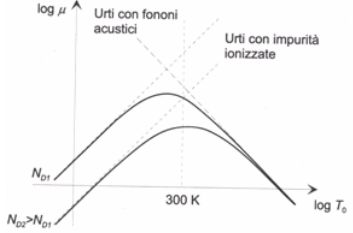
\includegraphics[scale=0.75]{Immagini_Micro&Nano/Imm_2_Fisica_dei_semiconduttori/2}
\end{center}
%
Quando al semiconduttore è applicato un campo elettrico di bassa intensità il parametro $\mu$ dipende dalle caratteristiche finisce del semiconduttore, in particolare a:
%
\begin{enumerate}
    \item urti con impurità ionizzate (ovvero al drogaggio)
    \item urti con fononi acustici (vibrazioni reticolari)
\end{enumerate}
%
I due meccanismi presentano un diverso comportamento in funzione della temperatura del reticolo.
Gli urti con impurità ionizzate hanno un tempo di rilassamento con andamento crescente rispetto alla temperatura, mentre gli urti con fononi acustici hanno un $\tau$ con andamento decrescente con la temperatura T.\\
Data quindi la presenza di due fenomeni non interagenti è possibile seguire una particolare regola che suggerisce il prevalere della mobilità $mu$ inferiore alle altre.\\
%
\begin{exbox}
    A basse temperature prevale al mobilità derivante da urti con impurità ionizzate dovute al drogaggio:
    Se faccio un drogaggio N, gli elettroni disponibili alla conduzione aumenteranno ma allora si avranno più cariche che si muoveranno poichè interagiscono con il campo elettrico dell'atomo drogante e quindi subiranno più rallentamenti e collisioni (è per questo che se N aumenta, mu diminuisce).
    A basse temperature, gli atomi del reticolo rimangono fermi, quindi gli unici a fornire contributo al numero di collisioni saranno gli elettroni mobili con gli atomi del drogaggio

\end{exbox}
%
\begin{exbox}
    A temperature elevate (intorno a 300K) prevale la mobilità derivante da urti con fononi acustici.\\
    All'aumentare di T, Il reticolo reagisce generando una vibrazione meccanica, cioè un'onda acustica che poi colpisce gli elettroni provocandone la spinta e la deviazione di traiettoria.
\end{exbox}
%
----------------
fig
\begin{center}
    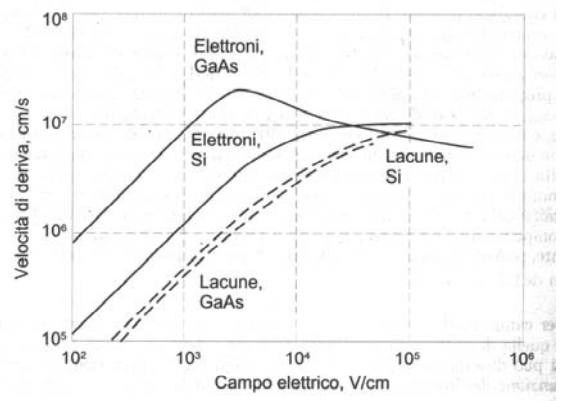
\includegraphics[scale=0.55]{Immagini_Micro&Nano/Imm_2_Fisica_dei_semiconduttori/3.png}
\end{center}

\subsection{Corrente di diffusione}

\begin{center}
    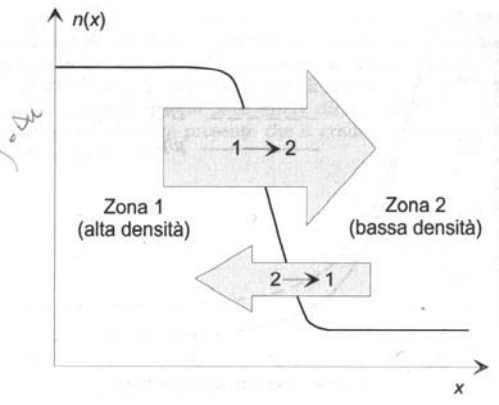
\includegraphics[scale=0.55]{Immagini_Micro&Nano/Imm_2_Fisica_dei_semiconduttori/5.png}
\end{center}
%
Poichè elettroni e lacune sono particelle cariche, pur rimanendo nell'intorno del loro punto di nascita, l'agitazione termica li fa muovere a destra e sx. A questo flusso di particelle è associato un flusso di carica e quindi una densità di corrente di diffusione:
%
\begin{align}
    \vec{J}_{n,d}&=qD_n\nabla_n\\
    \vec{J}_{h,d}&=-qD_h\nabla_p
\end{align}
%
dove $D_n$ è la diffusività degli elettroni e $D_p$ è la diffusività delle lacune.\\
L'equazione precedente sta  a dire che il gradiente di concentrazione produce una velocità media di diffusione del gasi di lacune ed elettroni pari a 
\begin{align}
    \vec{v}_{n,d}=-D_n \dfrac{\nabla n}{n}\\
    \vec{v}_{h,d}=-D_h \dfrac{\nabla p}{p}
\end{align}

la corrente misurabile totale è quindi la somma della corrente di deriva e di diffusione:

\begin{equation}
    \vec{J}_n^{TOT}=-qn\mu\mathcal{\vec{E}} + qD_n\nabla n
\end{equation}

\begin{psbox}
    se prendo un semiconduttore non connesso ad una batteria ($\vec{J}_n^{TOT}=0$) ma con un certo gradiente di concentrazione ($\nabla n \neq 0$), allora all'interno del semiconduttore si creerà un campo elettrico $\mathcal{\vec{E}}$ che bilancia la corrente di deriva e di diffusione in modo da soddisfare $\vec{J}_n^{TOT}=0$
\end{psbox}


\subsection{la relazione di Einstein}
La relazione di Einstein vale solo per semiconduttori non degeneri ed afferma che,\textit{in condizioni di equilibrio termodinamico e di basso campo $\mathcal{E}$, diffusività e mobilità sono proporzionali}. Questo è descritto dall'equazione di Einstein:
%
\begin{equation}
    D_n=\dfrac{k_B T_0}{q}\mu_{n0}
\end{equation}
%
\begin{equation}
    D_h=\dfrac{k_B T_0}{q}\mu_{h0}
\end{equation}
%
In condizioni di alto campo la diffusività si
discosta dalla relazione di Einstein; Mentre la mobilità tende a zero (infatti la velocità dei portatori satura) la diffusività tende ad un valore costante,
inferiore al valore di basso campo. 
%
\begin{figure}[hbt!]
    \centering
    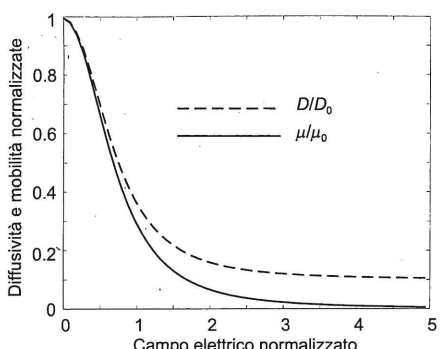
\includegraphics{Immagini_Micro&Nano/Imm_2_Fisica_dei_semiconduttori/grafico relazione di einstein.png}
    \caption{Caption}%
    \label{fig:enter_label}
\end{figure}
%
\cleardoublepage%

\section*{05/10/2023}
\section{Semiconduttori soggetti a perturbazione esterna}
Voglio studiare i diversi casi di semiconduttore soggetto a perturbazione esterna.
Prendo due equazioni. La prima è la densità di corrente di elettroni totale:
\begin{equation*}
    \vec{J}_n^{tot}=-qn \mu_n \mathcal{\vec{E}}+qD_n \dfrac{dn}{dx}
\end{equation*}

Dove, dalla equazione di Einstein abbiamo ricavato che
\begin{equation*}
    \mu_n=\dfrac{D_n}{V_T}
\end{equation*}
con
$V_T= \dfrac{k_B T}{q}\approx 25mV$\\
La seconda equazione necessaria per proseguire è chiamata "equazione di continuità" di elettroni e lacune:\\
Si consideri un insieme di cariche mobili in un mezzo materiale. Si supponga, in un primo momento, che le cariche mobili in gioco siano soggette solo al trasporto.
Siano allora Q la carica in un volume V, limitato da una superficie $\Sigma$ dotata di versore normale n diretto verso l'esterno, J la densità di corrente. La conservazione della carica totale Q implica:
\begin{equation}
    \dfrac{dQ}{dt}+\nabla J =0
\end{equation}

In realtà nel caso più generale devo considerare che le cariche in gioco siano soggette non solo al trasporto ma anche alla generazione-ricombinazione.
Pertanto, l'equazione di continuità deve essere arricchita con il terzo termine $U_Q$ chiamato tasso di ricombinazione/generazione. Questo parametro definisce la quantità di carica che scompare nell'unità di tempo per effetto della ricombinazione.
La conservazione della carica totale Q generale è:
\begin{equation}
     \dfrac{dQ}{dt}+\nabla J +U_Q=0
\end{equation}
L'equazione di continuità della carica può pertanto esprimersi come:
variazione temporale della carica volumica + divergenza della densità di corrente + tasso netto volumico di ricombinazione della carica = 0

\subsection{Tasso di Ricombinazione}
Questo Uq termine è legato a diversi fattori:
*) assorbimento di fotoni
*)collisione
*)trappole o difetti\\
L'equazione di ricombinazione e generazione$U_Q$ è meglio definita come segue:
\begin{equation*}
    U_Q=+G-R
\end{equation*}
Più precisamente si indicheranno i termini con pedice "n" nel caso di generazione e ricombinazione di elettroni e con pedice "h" nel caso di generazione e ricombinazione di lacune.\\
Parlando di elettroni:
\begin{equation*}
    U_{Qn}=G_n-R_n
\end{equation*}
La variazione di concentrazione di cariche in eccesso al variare del tempo è definito come:
\begin{equation*}
    \dfrac{dn'}{dt}=G_n-R_n
\end{equation*}
In caso di semiconduttore in condizione stazionaria la concentrazione di elettroni in eccesso è nullo, pertando generazione e ricombinazione si equivalgono.
\begin{equation*}
    0=G_n - R_n
\end{equation*}
Tuttavia, a causa di diversi motivi (quali sorgente luminose) può accadere ad un certo punto che ci sia elevata concentrazione di carica in eccesso. Allora accade che il tasso di ricombinazione è notevolmente maggiore della generazione ($G_n \gg R_n$) e quindi posso approssimare l'equazione in quella che si userà in seguito:
\begin{equation*}
    U_{Qn}=\dfrac{dn'}{dt}=-R_n
\end{equation*}
Ora rimane da trovare il valore di $R_n$:
\begin{equation*}
    R=\dfrac{n'}{\tau_n}
\end{equation*}
da cui
\begin{equation}
    \dfrac{dn'}{dt}=-\dfrac{n'}{\tau_n}
\end{equation}
%
Dove $\tau_n$ è il tempo di vita medio degli elettroni.\\
L'equazione, riporta il segno "-" ad indicare la diminuzione della densità di portatori di carica liberi nel tempo a causa della ricombinazione.\\
Con il passare del tempo il sistema si avvicina a uno stato stazionario ritornando, ancora una volta, alla condizione $G=R$.\\




%\cleardoublepage%

\subsection{Decadimento della concentrazione in eccesso dei portatori}

Considero un normale semiconduttore non drogato (intrinseco) di lunghezza W idealmente infinita. So che la concentrazione di cariche è uniforme lungo tutto il mezzo e di valore $n_i^2$.\\
E' interessante studiare i casi che provocano la variazione della concentrazione 
\begin{center}
    \begin{tikzpicture}[scale=0.75]
        \draw[fill={rgb:black,6;white,5}] (0,0)-- (5,0)-- (5,2)-- (0,2)-- (0,0);
        \draw[fill={rgb:black,4;white,7}] (0,2)-- (5,2)-- (4,3)-- (-1,3)-- (0,2);
        \draw[pattern=north east lines, pattern color=black] (0,0)-- (0,2)-- (-1,3)-- (-1,1)-- (0,0);       
        \draw[dashed] (-1,1)-- (4,1);
        \draw[dashed] (4,1)-- (4,3);
        \draw[dashed] (4,1)-- (5,0);

        %disegno radiazioni luminosa
        \draw[->,decorate,decoration={snake,amplitude=.4mm,segment length=2mm,post length=1mm}] (-2.5,2) --++ (1,0);
        \draw[->,decorate,decoration={snake,amplitude=.4mm,segment length=2mm,post length=1mm}] (-2.5,1.7) --++ (1,0);
        \draw[->,decorate,decoration={snake,amplitude=.4mm,segment length=2mm,post length=1mm}] (-2.5,1.4) --++ (1,0);

        %label energia fotoni
        \node at (-3.5,1.7) [scale=1.5]{$h \nu$};

        %disegno asse x
        \draw[thick,->] (0,-4) node[anchor=north]{$0$}--++ (6,0)
        node[anchor=west]{$x$};
        %disegno asse y
        \draw[thick,->] (0,-4)--++ (0,3) node[anchor=south]{$n(x)$};
        %disegno i grafici
        \draw[dashed] (0,-3.25) --++ (5,0);
        %\draw[ domain=0:5, color=red, thick, ->, samples=500] plot (\x, {exp(-\x + 0.3)} - 3.2);
        \draw[thick, red] (-0.5, -2.8) .. controls (1, -3.1) and (2, -3.3) .. (3, -3.4) .. controls (4, -3.45) and (5, -3.48) .. (5.5, -3.49);

        %label e doppia freccia
        \draw[dashed] (0,-1.85) --++ (-0.2,0) node[anchor=east]{$n_i^2+n'$};
        \draw[dashed] (0,-3.25) --++ (-0.2,0) node[anchor=east]{$n_i^2$};
        \draw[<->] (-0.2,-1.85) -- (-0.2,-3.25);
        \draw[->] (0,-4.0) -- ++ (1.5,0) node[anchor=north]{$L_n$};
    \end{tikzpicture}
\end{center}
\subsubsection*{1°Caso) Semiconduttore non drogato esposto a sorgente luminosa}
Considero un semiconduttore illuminato da una sorgente di fotoni sulla faccia posta in x=0 inoltre:
\begin{itemize}
    \item Assumo di avere fotoni ad alta energia in modo da garantire il passaggio degli elettroni dalla banda di valenza alla banda di conduzione, quando assorbono tale energia;
    %
    \item il campione è mantenuto in condizioni di circuito aperto (senza generatore collegato), ossia la corrente che fluisce nel campione è nulla in ogni sezione;
\end{itemize}
%
La pioggia di fotoni provoca una generazione superficiale di portatori in eccesso pari a $n'$ in $x=0$; questo eccesso di elettroni si smaltisce all'aumentare di x fino a quando, per $x=+\infty$, la perturbazione generata dai fotoni si è completamente annullata ($n'=0$).\\

Faccio un'ulteriore semplificazione considerando due ipotesi:\\
\begin{itemize}
    \item [\textbf{Hp.1}] il sistema è in condizioni stazionarie\\
        Questo significa che non ci sono variazioni di carica nel tempo $(\dfrac{dQ}{dt}=0)$\\
    \item [\textbf{Hp.2}] Il campo elettrico esterno è nullo $\mathcal{\vec{E}}=0$\\
        Questo implica che la corrente di deriva (detta di trascinamento) diventi, in prima approssimazione, trascurabile
\end{itemize}
Unendo l'equazione  $J_n^{tot}$ all'equazione di continuità e usando le precedenti ipotesi ottengo il seguente sistema:
%
\begin{alignat*}{4}[left = \empheqlbrace]
   0 + \dfrac{d\vec{J}^{\text{tot}}}{dx} - R_n = 0  \\
    \vec{J}^{\text{tot}}= q\,D_n \cdot \frac{dn'}{dx}
\end{alignat*}
%
La forma a cui si giunge è una EDO omogenea:
%
\begin{equation}
    D_n \cdot \dfrac{d^2 n'}{dx^2}= \dfrac{n'}{\tau_n}
\end{equation}
%
\begin{ripasso}[come risolvere l'EDO:]
La soluzione generale della EDO è:
\begin{equation*}
    n'(x)=A\cdot \exp \left( \dfrac{x}{L_n}\right) + B \cdot \exp \left( \dfrac{-x}{L_n} \right)
\end{equation*}

Le costanti A e B possono essere determinate imponendo le condizioni al contorno:
\begin{align*}
    n'(0)&=n_i^2+n' \\
    n'(\infty)&=n_i^2
\end{align*}

Pertanto
\begin{align*}
    n'(0)&=A+B=n_i^2+n'\\
    n'(\infty)&=A\cdot \infty+B=n_i^2
\end{align*}

Dall'ultima equazione si evince che $A=\dfrac{n_i^2-B}{\infty}=0$ ; mentre dalla prima si ottiene che $B=n'(0)$.\\
\end{ripasso}
%
Allora il risultato finale è l'equazione di diffusione dei portatori minoritari risulta:
\begin{equation}
    n'(x)=n'(0) \cdot \exp \left( \dfrac{-x}{L_n}\right)
\end{equation}

Dove $L_n=\sqrt{D_n \tau_n}$ è detta lunghezza di diffusione degli elettroni.\\
Quindi si osserva che, in presenza di iniezione laterale di portatori in eccesso, \textbf{le concentrazioni di eccesso tendono ad annullarsi con legge esponenziale decrescente} con una lunghezza tipica $L_n$  tanto maggiore quanto più lungo il tempo medio dei portatori in eccesso.\\
La corrente di diffusione vale:
%
\begin{equation}
    J_{n,d}(x)=qD_n \dfrac{dn'(x)}{dx}=qD_n \dfrac{d}{dx}\left( n'(0) e^{\dfrac{-x}{L_n}}\right)=-q\sqrt{\dfrac{D_n}{\tau_n}}(n_i^2+n')\exp(-x/L_n)
\end{equation}
%
La corrente di lacune corrispondente tale da soddisfare la condizione di quasi neutralità si scrive:
%
\begin{equation}
    J_{h,d}(x)=-qD_h \dfrac{dp'(x)}{dx}=\dfrac{qD_h}{L_h}(n_i^2+n')\exp(-x/L_h)=q\sqrt{\dfrac{D_h}{\tau_h}}(n_i^2+n')\exp(-x/L_h)
\end{equation}
%
E' quindi importante notare che se le due correnti sono uguali e contrarie, allora i tempi di vita media e la diffusività di elettroni e lacune sono uguali. in questo caso la corrente totale è nulla ed è quindi rispettata la condizione di circuito aperto alla parete sinistra del semiconduttore. \\
%
\textbf{Se questo non accadesse, significherebbe che le due correnti di diffusione sono differenti e si stabilirebbe quindi una condizione di non neutralità che a sua volta genera un campo elettrico tale da provocare una corrente di deriva che renda nulla la corrente totale}.

Mi interessa analizzare il comportamento di un semiconduttore in presenza di uno scostamento dalla neutralità nel tempo e nello spazio.\\
Per permettere una semplice analisi quantitativa si suppone che lo scostamento sia piccolo, ossia che il semiconduttore operi in condizioni di piccolo segnale.\\
Consideriamo due casi di scostamento della neutralità:
%
\begin{enumerate}
    \item scostamento dalla neutralità uniforme nello spazio ma dipendente dal tempo (tempo-variante);
    \item scostamento dalla neutralità uniforme nel tempo ma dipendente dallo spazio.
\end{enumerate}
%
Per entrambi i casi si considera un semiconduttore drogato di tipo n e monodimensionale (direzione solo lungo le x, per semplificare le operazioni di derivazione)\\

\paragraph{Scostamento dalla neutralità nel tempo}\mbox{}\\
Se ho un semiconduttore drogato con una concentrazione di atomi donori pari ad $N_D$ (ed uno di questi dona 1 elettrone), la concentrazione di elettroni nel tempo sarà circa il numero di atomi donori più i portatori in eccesso:
%
\begin{align}
    n(t)&=n_0+n'(t)\approx N_D+n'(t)
\end{align}
%
\begin{align*}
    (n'&\ll n_0 )
\end{align*}
%
Dove la concentrazione degli elettroni $n_0$ è assunta uguale alla concentrazione di atomi donori $N_D$, mentre $n'(t)$ rappresenta l'eccesso locale di elettroni sul SC drogato nel caso, di un altro SC maggiormente drogato posto a contatto.\\
La concentrazione delle lacune rimane invariata:
%
\begin{align}
    p(t)&=p_0
\end{align}
%
\begin{align*}
    (p_0&\ll n_0)
\end{align*}
%
\begin{psbox}[ATTENZIONE]
 $p(t)=p_0 \neq p_i$
Infatti, per la legge di azione di massa, in un generico semiconduttore: $n\cdot p=n_i \cdot p_i$ ;
quindi se $n\uparrow$, necessariamente $p\downarrow$ in modo da mantenere soddisfatta l'equivalenza.
Pertanto, nel caso di semiconduttore drogato n si avrà che:
il numero di elettroni aumenta ($n=n_0=N_D$ )e il numero di lacune diminuisce ($p=p_0 $)
\end{psbox}
%
L'eccesso locale di elettroni causa una variazione del campo elettrico e quindi del potenziale $\phi(t)$:
%
\begin{equation}
    \phi(t)=\phi_0+\phi'(t)
\end{equation}
Ricordo che sto studiando il caso semplice di semiconduttore omogeneo (per cui la variazione di $n$ è indipendente nello spazio: $\dfrac{dn}{dx}=0$) ovvero sto trascurando la corrente diffusiva, allora la densità di corrente di elettroni vale: 
%
\begin{equation}
    J_n=-qn \mu_n \dfrac{d\phi}{dx}
\end{equation}
%
Adesso inserisco $J_n$ nell'equazione di continuità trascurando l'effetto della ricombinazione-generazione (poiché ci sono talmente tante cariche che$ \dfrac{n'}{\tau}\rightarrow 0$), ottenendo:
%
\begin{align}
    q \dfrac{dn}{dt} &+\nabla \cdot J_n=0\\
    q \left[ \dfrac{dN_D}{dt} + \dfrac{dn'(t)}{dt}\right] &+ \nabla \cdot \left[ -qn\mu_n \dfrac{d\phi}{dx} \right] = 0 \nonumber\\
    q \left[ 0 + \dfrac{dn'(t)}{dt}\right] &+ \nabla \cdot \left[ -qn\mu_n \dfrac{d\phi}{dx} \right] = 0 \nonumber\\
    q \dfrac{dn'(t)}{dt} &= qn \mu_n \left[ \nabla \cdot \dfrac{d\phi}{dx} \right] \nonumber
\end{align}
%
In conclusione 
%
\begin{equation}
    \dfrac{n'(t)}{dt}=\mu_n n \dfrac{d^2 \phi}{dx^2}
\end{equation}
%
Questa equazione assomiglia molto ad una EDO, peccato la presenza di due variabili sotto le derivate.
Tuttavia, in questa equazione posso applicare una semplificazione considerando che all'interno cé la cosiddetta equazione di Poisson:
%
\begin{equation}
    \dfrac{d^2 \phi}{dx^2} = \dfrac{q}{\epsilon}n'(t)
\end{equation}
%
Pertanto, l'eccesso nel tempo avrà forma:
%
\begin{equation}
    n'(t)=n'(0)+\exp \left[ \frac{-t}{\tau_D} \right]
\end{equation}
%
Dove $\tau_D= \dfrac{\epsilon}{qN_d \mu_n}= \dfrac{\epsilon}{\sigma_n}$ è detto tempo di
rilassamento dielettrico. Il parametro $\sigma_n$ è la conducibilità elettrica del
semiconduttore dovuta ai soli elettroni, che equivale in questo caso alla 
conducibilità totale.\\
%
\begin{psbox}[NOTA]
Dall'equazione precedente si nota che 
$\tau_D$  $1/\alpha$  $ \mu$, $ N_D$\\
Pertanto, aumentare la concentrazione di atomi donori oppure la mobilità dei portatori, significa anche aumentare la velocità di ritorno alla condizioni di equilibrio che corrisponde ad avere un dispositivo che risponde (o commuta) più velocemente.\\
Ogni materiale ha un suo tempo di rilassamento \\
FIGURE SBAGLIATE MA BELLE.\\
e nel caso limite si ha il pec, un metallo caratterizzato da $\tau_D \approx 0$:
Quando $V_{bias}$ smette di variare, gli elettroni in eccesso verranno riassorbiti nel tempo $\tau_D$, in questo caso sarà pressochè istantaneo.
%
\noindent\begin{minipage}{0.49\textwidth}
    \begin{center}
    \begin{circuitikz}
    \draw(-0.5,0) to [american voltage source, v=$V_{bias}$,invert] (0,0)--++ (0.5,0);
        \draw[pattern= north east lines] (0.5,0.5) rectangle (1,-0.5);
        \draw(1,0.5) rectangle (3,-0.5);
        \draw(3,0)--++ (0.5,0) to (3.5,-0.5) node[tlground]{};
        %disegno asse x
        \draw[thick,->] (1,-0.7) node[anchor=north]{$0$}--++ (2,0)
        node[anchor=north ]{$x$};
        %disegno asse y
        \draw[thick,->] (1,-0.7)--++ (0,2) node[anchor=south]{$n'(x)$};
        %disegno i grafici
        %\draw[smooth, domain=0:4, color=red, thick] plot (\x, {exp(-\x + 0.3) - 1});

    \end{circuitikz}
\end{center}
\captionof{figure}{CaptionA}
\end{minipage}
\hfill%
\begin{minipage}{0.49\textwidth}\raggedleft
    \begin{center}
    \begin{circuitikz}
    \draw(-0.5,0) to [american voltage source, v=$V_{bias}$,invert] (0,0)--++ (0.5,0);
        \draw[pattern= north east lines] (0.5,0.5) rectangle (1,-0.5);
        \draw(1,0.5) rectangle (3,-0.5);
        \draw(3,0)--++ (0.5,0) to (3.5,-0.5) node[tlground]{};
        %disegno asse x
        \draw[thick,->] (1,-0.7) node[anchor=north]{$0$}--++ (2,0)
        node[anchor=north ]{$x$};
        %disegno asse y
        \draw[thick,->] (1,-0.7)--++ (0,2) node[anchor=south]{$n'(x)$};
        %disegno i grafici
        %\draw[smooth, domain=0:4, color=red, thick,scale=0.5] plot (\x+2,{\exp((-\x+0.3)) -1});
    \end{circuitikz}
\end{center}
\captionof{figure}{Caption B}
\end{minipage}
%
\end{psbox}
%
\cleardoublepage%

\paragraph{Scostamento dalla neutralità nello spazio}
Per uno scostamento dalla neutralità costante nel tempo ma funzione dello spazio si può scrivere:

\begin{align}
    n(x)&=n_0+n'(x)\approx N_D+n'(x)
\end{align}
\begin{align*}
    (n'&\ll n_0 )
\end{align*}
Dove la concentrazione degli elettroni $n_0$ è assunta (anche giustamente) uguale alla concentrazione di atomi donori $N_D$.
Dove $n'(x)$ rappresenta l'eccesso locale di elettroni sul SC drogato nel caso, per esempio, di un altro SC maggiormente drogato posto a contatto.
La concentrazione delle lacune rimane invariata:
\begin{align}
    p(x)&=p_0
\end{align}
\begin{align*}
    (p_0&\ll n_0)
\end{align*}

PS: su $p(x)$ vale l'osservazione del caso precedente.

L'eccesso locale di elettroni nello spazio causa una variazione di potenziale $\phi(x)$:
\begin{equation}
    \phi(x)=\phi_0+\phi'(x)
\end{equation}
Si va a considerare J (questa volta ci sarà una corrente diffusiva a causa della variazione di concentrazione di elettroni dello spazio):

\begin{equation}
    J_n=-q \mu_n n \dfrac{d\phi}{dx}+qD_n \frac{dn}{dx}
\end{equation}

e lo si inserisce nell'equazione di continuità trascurando l'effetto della ricombinazione-generazione (poiché ci sono talmente tante cariche che $ \dfrac{n'}{\tau}\rightarrow 0$) e trascurando la variazione di carica nel tempo (poiché stiamo considerando il caso di neutralità costante nel tempo: $\dfrac{dQ}{dt}=0$):
\begin{align}
    \nabla J_n=0
\end{align}
Risolvendo:
\begin{align}
    \nabla \cdot \left[ q \mu_n n \dfrac{d \phi}{dx} + q D_n \dfrac{dn}{dx}\right] &=0 \nonumber\\
    -q \mu_n n \nabla \cdot \dfrac{d\phi}{dx}       + qD_n \nabla \cdot \frac{dn}{dx}&=0 \nonumber\\
    qD_n \nabla \cdot \left[ \frac{dN_D}{dx} + \dfrac{dn'(x)}{dx} \right] &= q \mu_n n \nabla \cdot
    \dfrac{d\phi}{dx} \nonumber\\
    qD_n \nabla \cdot \left[ \frac{dN_D}{dx} + \dfrac{dn'(x)}{dx} \right] &= q \mu_n n \nabla \cdot 
    \dfrac{d\phi}{dx} \nonumber
\end{align}
In conclusione, 
\begin{equation}
    D_n \dfrac{d^2 n'(x)}{dx^2}= \mu_n n \dfrac{d^2\phi}{dx^2}
\end{equation}

Questa equazione assomiglia molto ad una EDO, peccato che non posso risolverla così com'è perchè ci siano due variabili diverse sotto derivata
Tuttavia, in questa equazione posso applicare una semplificazione considerando che all'interno cé la cosiddetta equazione di Poisson: 
\begin{equation}
    \dfrac{d^2 \phi}{dx^2} = \dfrac{q}{\varepsilon}n'(t)
\end{equation}

Pertanto, l'eccesso nel tempo avrà forma:
\begin{equation}
    n'(t)=n'(0)+\exp \left[ \frac{-x}{L_D} \right]
\end{equation}

Dove $L_D=\sqrt{\dfrac{\varepsilon k_B T_0}{q^2 N_D}}$ è detta lunghezza di Debye. \\
\begin{exbox}[Un pò di numeri]
Nel silicio a temperatura ambiente:
\begin{align*}
    N_D&=10^{-16} && \,cm^{-3}\\
    \mu_n&=10^{3} && \,cm^{2}/s\\
    L_D&=10^{-8}  && \,m\\
    \tau_D&=10^{-13} && \,s
\end{align*}
    Proff figura?
\end{exbox}

Quindi che le perturbazioni locali o temporali dalla neutralità tendono  a smorzarsi con tempo dell'ordine del tempo di rilassamento dielettrico i in lunghezze dell'ordine della lunghezza di Debye, quando non vengano mantenute da cause esterne(caso giunzione polarizzata).\\

Con questi strumenti sono in grado di studiare bene come operano tre tipi di giunzione molto importanti:
\begin{enumerate}
    \item giunzione tra due semiconduttori uguali ma con drogaggio diverso (giunzione PN) $(E_{g1} =E_{g2})$
    \item giunzione tra metallo e semiconduttore $(E_{g,metal} =0 ; E_{g1})$
    \item giunzione tra due semiconduttori completamente diversi tra solo $(E_{g1} \neq E_{g2} )$
\end{enumerate}
\cleardoublepage%

\noindent\begin{minipage}{0.9\textwidth}
    \section{giunzione tra due semiconduttori uguali ma con drogaggio diverso, il diodo P-N}
\end{minipage}
\begin{minipage}{0.1\textwidth}\raggedleft
    \begin{pgGhione}
    255
    \end{pgGhione}
\end{minipage}

\subsection{studio qualitativo}
figura
il semiconduttore N ha un livello di fermi più alto, rendendo più semplice il passaggio degli elettroni dalla banda di valenza alla banda di conduzione, e viceversa.\\
Nel caso in cui due semiconduttori con livelli di energetici diversi vengano messi a contatto, i livelli energetici di fermi si stabilizzano ad un valore costante:
Ma se il livello di fermi deve rimanere costante, tutto il resto dovrà cambiare\\
\begin{figure}[hbt!]
    \centering
    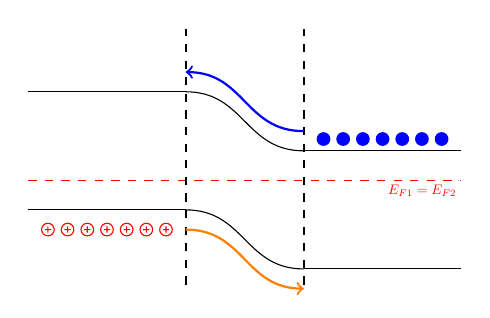
\begin{tikzpicture}[scale=0.5,transform shape]
        %disegno l'unione di due SC
        %mezzo 1
        \draw(0,3) --++ (4,0);
        \draw(0,0) --++ (4,0);
        %mezzo 2
        \draw(7,1.5) --++ (4,0);
        \draw(7,-1.5) --++ (4,0);
        %livello di fermi
        \draw[dashed, red] (0,0.75) --++ (11,0) node[anchor=north east]{$E_{F1}=E_{F2}$};
        %intersezione
        \draw[] (4,3)..controls (5.5,3) and (5.5,1.5).. (7,1.5);
        \draw[] (4,0)..controls (5.5,0) and (5.5,-1.5).. (7,-1.5);
        %lacune
        \foreach \pos in {0.5,1,1.5,2,2.5,3,3.5} {
        \node at (0+\pos,-0.5) { \tikz\draw[thick,red]
          circle (0.16cm) (-0.08,0)-- (0.08,0) (0,0.08)-- (0,-0.08) ;} ;}
        %elettroni
          \foreach \pos in {0.5,1,1.5,2,2.5,3,3.5} {
        \node at (7+\pos,+1.8) { \tikz\draw[thick,blue, fill=blue]
          circle (0.16cm)  ;} ;}
        %delimitazioni
        \draw[thick, dashed] (4,-1.9)--++ (0,6.5);
        \draw[thick, dashed] (7,-1.9)--++ (0,6.5);
        %altro
        \draw[blue,thick,<-]
        (4,3.5)..controls (5.5,3.5) and (5.5,2).. (7,2);
        \draw[orange,thick,->]
        (4,-0.5)..controls (5.5,-0.5) and (5.5,-2).. (7,-2);
    \end{tikzpicture}
    \caption{Caption}%
    \label{fig:enter_label}
\end{figure}
Figura e spiegazione\\
Ricavo che dalla zona P si avrà un eccesso di lacune, una piccolissima quantità di elettroni liberi ed una grandissima quantità di ioni negativi denominate cariche stazionarie (o ioni accettori fissi). Trascurando l'effetto di questi pochi elettroni liberi, posso dire che le lacune sono bilanciate dalle cariche stazionare negative per rendere la zona elettricamente neutra.\\
Il ragionamento è duale per quanto riguarda la regione drogata tipo N (con gli equivalenti ioni donori fissi) .\\

%
\noindent\begin{minipage}{0.55\textwidth}
Nel memento in cui questi due mezzi sono posti a contatto, a cavallo della giunzione si presenta una differenza di concentrazione delle lacune fra zona P e zona N, rappresentate rispettivamente con Na ed Nd.
Questo gradiente produce una diffusione di lacune che dalla zona drogata P si diffondono verso quella drogata N.\\
le stesse considerazioni valgono per gli elettroni liberi in zona N.\\
Questo fenomeno di diffusione presenta importanti conseguenze;
ricordo che le due zone sono elettricamente neutre, cioè per ogni elettrone (lacuna) nella zona N (P) ci sarà uno ione fisso positivo (ione fisso negativo).
Appena il primo elettrone libero si sposta dalla zona N ed arriva in zona P, trasportando con sé la propria carica elettrica, esso produce un'alterazione della neutralità di carica: la zona P si ritrova con una carica negativa in più, mentre la zona N se ne ritrova una in meno.
Ciò crea a cavallo della giunzione, un campo elettrico diretto verso P.\\
\end{minipage}
\hfill%
\begin{minipage}{0.4\textwidth}\raggedleft
    \begin{center}
    \begin{tikzpicture}[scale=0.45,transform shape]
         %disegno asse x
        \draw[->] (-4,0) node[anchor=north]{}--++ (9,0)
        node[anchor=west]{$x$};
        %disegno asse y
        \draw[->] (0,-4)--++ (0,8) node[anchor=south west]{$\rho_{fissa}$};
        %disegno grafici
        \draw[thick,pattern=north east lines, pattern color=gray] (0,0)rectangle++ (3,3);
        \draw[thick,pattern=north east lines, pattern color=gray] (0,0)rectangle++ (-2,-3);
        %label
        \node at (3,0) [anchor=north]{$x_n$};
        \node at (-2,0) [anchor=south]{$-x_p$};
        \node at (0,3) [anchor=east]{$N_D$};
        \node at (0,-3) [anchor=west]{$N_A$};

        %disegno l'energia
        \draw[thick,red] (-4,0.03)-- (-2,0.03)-- (0,-3)-- (3,0.03)-- (5,0.03);

        %disegno grafico potenzili
        %disegno asse x
        \draw[->] (-4,-9) node[anchor=north]{}--++ (9,0)
        node[anchor=west]{$x$};
        %disegno asse y
        \draw[->] (0,-12)--++ (0,7) node[anchor=south west]{$\phi$};
        
        %disegno graficiù
        \draw[blue] (-2,-9)..controls (1,-9) and (-2,-7.5).. (3,-7.5)--++ (2,0);
        \draw[red] (-2,-9)..controls (1,-9) and (-2,-11.1).. (3,-11)--++ (2,0);
    
        %tratteggi
        \draw[dashed] (-2,0)--++ (0,-9);
        \draw[dashed] (3,0)--++ (0,-9);
        %label
        \draw[<->,blue] (4,-9)-- (4,-7.5);
        \node at (4,-8.25)[anchor= west,blue]{$\phi_{Bi}$};
        \draw[<->,red] (4,-11)-- (4,-9);
        \node at (4,-10)[anchor= west,red]{$-q\phi_{Bi}$};
    \end{tikzpicture}
    \captionof{figure}{Caption}
\end{center}
\end{minipage}

%

Ulteriori passaggi di elettroni verso la zona P (e lacune verso la zona N) contribuiranno ad alterare la neutralità delle zone e quindi a rendere più forte il campo elettrico, il quale spinge verso destra gli elettroni e verso sinistra le lacune riducendo la corrente di diffuzione fino a trovare una situazione di equilibrio in cui la forza del campo elettrico eguaglia la spinta esercitata dalla diffusione.\\

La presenza del campo elettrico produce una differenza di potenziale a cavallo della giunzione che va via aumentando con l'aumentare delle cariche che accumulano ai lati della giunzione stessa. A destra si addensano cariche positive, emntre a sinistra cariche negative.
Questa differenza è chiamata barriera di potenziale per indicare che essa si pone come barriera ai portatori di carica soggetti alla psinta della diffuzione .
La barriera auemnta fino a quando i portatori che diffondono non sono più in grado di superarla.\\
\begin{figure}[hbt!]
    \centering
\begin{tikzpicture}[scale=0.75, transform shape]
    %disegno asse x
        \draw[->] (-5,0)--++ (10,0)
        node[anchor=west]{$x$};
        %disegno asse y
        \draw[->] (0,-1)--++ (0,5) node[anchor=south west]{$\rho_{mobile}$};
        %disegno tratteggi
        \draw[dashed] (-2,0)--++ (0,4);
        \draw[dashed] (2,0)--++ (0,4);
        %disegno grafici
        \draw[thick, red] (-5,0.5)-- (-2,0.5)  (2,0.5)-- (5,0.5);
        \draw[thick, black] (-5,3)-- (-2,3)  (2,3)-- (5,3);
        %label 
        \node at (-2,0)[below]{$-x_p$};
        \node at (2,0)[below]{$x_n$};
        
        \node at (-5,3)[left]{$N_A$};
        \node at (-5,0.5)[left]{$nP_0$};
        
        \node at (5,3)[right]{$N_D$};
        \node at (5,0.5)[right]{$Pn_0$};
\end{tikzpicture}
    \caption{Caption}%
    \label{fig:enter_label}
\end{figure}

Per costruire il diagramma a bande bisognerà ricordare che:
\begin{enumerate}
    \item la densità di elettroni e lacune dipende da $E_F$ secondo le relazioni:
            \begin{align*}
                n=N_C \cdot \exp\left (\dfrac{E_F-E_C}{k_B T} \right)\\
                p=N_V \cdot \exp\left (\dfrac{E_V-E_F}{k_B T} \right)
            \end{align*}
    \item esiste un campo elettrico nei dintorni della giunzione, indicando che le bande saranno inclinate
            In tale regione il numero di elettroni in zona n e di lacune in zona p sono sensibilmente 
            inferiori rispetto al loro valore lontano dalla giunzione (zona di svuotamento).
            
\end{enumerate}

Poiché n è esponenzialmente dipendente dalla distanza $E_C-E_F$ (e p da $E_F-E_V$) allora, nel diagramma, $E_C$ si allontana dalla zona $E_F$.
Perciò il campo elettrico fa inclinare le bande, mentre il livello di fermi resta piatto e costituisce un comodo livello di riferimento per il potenziale\\
Figura\\

Per quanto abbiamo detto, Il diagramma a bande in equilibrio termodinamico rivela che in corrispondenza della giunzione vi è un campo elettrico di built-in;
questo contrasta la tendenza degli elettroni a diffondersi dal lato n al lato p e delle lacune a diffondersi dal lato p al lato n, in modo tale da rendere nulla la corrente totale, come richiesto dalla condizione di equilibrio termodinamico.

Pertanto, la corrente di deriva indotta dal campo di built in compensa esattamente la corrente di diffusione indotta dai gradienti di concentrazione dei portatori.

quando si uniscono si una una cetra concentrazione di ioni fissi:\\
fig\\

il campo elettrico sarà\\
fig\\
La conseguenza della presenza del campo elettrico è l'esistenza di un potenziale. Sappiamo infatti che esso è legato al campo elettrico dall'equazione
\begin{equation}
    \mathcal{\vec{E}}(x)=-\nabla V(x)
\end{equation}
Considerando l'impotesi modonimensionale:
\begin{equation}
    \mathcal{\vec{E}}(x)=-\dfrac{V(x)}{dx}
\end{equation}

Da cui 
\begin{equation}
    V(x)= \int_{-\infty}^{x}\mathcal{\vec{E}}(x)dx
\end{equation}

All'equilibrio termodinamico tra i due lati della giunzione si ha una differenza di potenziale Vbi. Come si calcola?

Il valore Vbi si può dedurre imponendo che la densitò di corrente per gli elettroni si annilli all'equilibrio termico
\begin{equation}
    J_n=J_{n,Deriva} + J_{n,Diffusione} = q \mu_n n \mathcal{\vec{E}}(x) +qD_n \dfrac{dn}{dx}
\end{equation}

Il che implica
\begin{equation}
    \mathcal{\vec{E}}(x) = - \dfrac{D_n}{\mu_n} \dfrac{1}{n} \dfrac{dn}{dx}= -\dfrac{KT}{q}\dfrac{1}{n} \dfrac{dn}{dx}
\end{equation}

Da cui si può ricavare Vbi
\begin{equation}
   % V_bi=-∫_(-∞)^(+∞)▒E(x)  dx=KT/q ln((N_D N_A)/(n_i^2 ))
\end{equation}


\subsection{DIAGRAMMA A BANDE IN POLARIZZAZIONE DIRETTA}
In equilibrio termodinamico sottoponiamo la giunzione pn a polarizzazione diretta, ossia applichiamo al lato p un potenziale positivo, mantenendo il lato n al potenziale di riferimento.
Di seguito considereremo il caso di filo ideale. l'intera tensione fornita dal generatore cade sulla regione di carica spaziale.

Se il lato p è polarizzato positivamente, l'energia potenziale del mezzo p diminuisce.
Supponendo di mantenere come riferimento il livello delle bande del lato n, la tensione applicata $V_A>0$ riduce la barriera di potenziale a XX causando una riduzione del campo di built in
\begin{figure}[hbt!]
    \centering
    \begin{tikzpicture}
    %disegno asse x
        \draw[->] (-5,0)--++ (10,0)
        node[anchor=west]{$x$};
        %disegno asse y
        \draw[->] (0,-1)--++ (0,5) node[anchor=south west]{$\rho_{mobile}$};
        %disegno tratteggi
        \draw[dashed] (-2,0)--++ (0,4);
        \draw[dashed] (2,0)--++ (0,4);
        %disegno grafici
        \draw[thick, red] (-5,0.5)-- (-2,0.5)  (2,0.5)-- (5,0.5);
        \draw[thick, black] (-5,3)-- (-2,3)  (2,3)-- (5,3);
        %collegamenti
        \draw[blue] (-2,3)..controls (-0.5,3) and (0.5,0.5).. (2,0.5);
        \draw[green] (-2,0.5)..controls (-0.5,0.5) and (0.5,3).. (2,3);
        %label 
        \node at (-2,0)[below]{$-x_p$};
        \node at (2,0)[below]{$x_n$};
        
        \node at (-5,3)[left]{$N_A$};
        \node at (-5,0.5)[left]{$nP_0$};
        
        \node at (5,3)[right]{$N_D$};
        \node at (5,0.5)[right]{$Pn_0$};
\end{tikzpicture}
    \caption{Caption}%
    \label{fig:enter_label}
\end{figure}
%
\begin{figure}[hbt!]
    \centering
    \begin{tikzpicture}
    %disegno asse x
        \draw[->] (-5,0)--++ (10,0)
        node[anchor=west]{$x$};
        %disegno asse y
        \draw[->] (0,-1)--++ (0,5) node[anchor=south west]{$\rho_{mobile}$};
        %disegno tratteggi
        \draw[dashed] (-2,0)--++ (0,4);
        \draw[dashed] (2,0)--++ (0,4);
        %disegno grafici
        \draw[thick, red] (-5,0.5)-- (-2,0.5)  (2,0.5)-- (5,0.5);
        \draw[thick, black] (-5,3)-- (-2,3)  (2,3)-- (5,3);
        %collegamenti
        \draw[blue] (-2,3)..controls (0.5,3) and (-0.5,0.5).. (2,0);
        \draw[blue] (2,0)..controls (3,0) and (3.7,0.5).. (5,0.5);
        
        \draw[green] (-2,0)..controls (0,0.5) and (0,3).. (2,3);
        \draw[green] (-5,0.5)..controls (-3.7,0.5) and (-3,0).. (-2,0);
        %label 
        \node at (-2,0)[below]{$-x_p$};
        \node at (2,0)[below]{$x_n$};
        
        \node at (-5,3)[left]{$N_A$};
        \node at (-5,0.5)[left]{$nP_0$};
        
        \node at (5,3)[right]{$N_D$};
        \node at (5,0.5)[right]{$Pn_0$};
\end{tikzpicture}
    \caption{Caption}%
    \label{fig:enter_label}
\end{figure}
\cleardoublepage%

\section*{09/10/2023}

\subsection{Tensione di built-in (analisi quantitativa) pg 265}
Considero di avere una giunzione fra due semiconduttori con elevato drogaggio, cioè con drogaggio molto maggiore di quello che ci sarebbe in n semiconduttore intrinseco. il semiconduttore P avrà livello di fermi molto minore di quello intrinseco mentre il semiconduttore N avrà un livello di fermi molto maggiore.
utilizzando la forma di Shockley (ossia prendendo come riferimento per il potenziale il livello di Fermi intrinseco), si ha:

\begin{align*}
    n_0(x)=n_i \cdot \exp\left (\dfrac{E_F-E_{Fi}(x)}{k_B T} \right)\\
    p_0(x)=n_i \cdot \exp\left (\dfrac{E_{Fi}(x)-E_F}{k_B T} \right)
 \end{align*}\\
 Dove il pedice "0" indica la condizione di equilibrio termodinamico.\\
 Lontano dalla giunzione, le concentrazioni di elettroni e lacune sono, rispettivamente, circa uguali alle concentrazioni di donatori e accettori. Per cui valgono le relazioni:
\begin{align}
    n(\infty)=N_D=n_i \cdot \exp\left (\dfrac{E_F-E_{Fi}(+\infty)}{k_B T} \right)\\
    p(\infty)=N_A=n_i \cdot \exp\left (\dfrac{E_{Fi}(-\infty)-E_F}{k_B T} \right)
 \end{align}
Estrapolando i livelli energetici presenti all'esponenziale, ottengo:
 \begin{align}
     E_F-E_{Fi}(+\infty) = k_B T \log \left({\dfrac{N_D}{n_i}} \right)\\
     E_{Fi}(-\infty)-E_F = k_B T \log \left({\dfrac{N_A}{n_i}} \right)
 \end{align}\\
Se ora facciamo la somma di queste due equazioni (e $V_A=0$), trovo:
 \begin{equation}
     qV_{bi}=E_{Fi}(-\infty)-E_{Fi}(+\infty)=k_B T \log \left( \dfrac{N_D N_A}{n_i^2}\right)
 \end{equation}\\
Mettendo tutto insieme trovo:
 \begin{align}
 \label{eqn:Vbi}
      V_{bi}= \dfrac{k_B T}{q}\log \left( \dfrac{N_D N_A}{n_i^2}\right)
 \end{align}

Dall'espressione della $V_{bi}$ capisco che, fissato il semiconduttore intrinseco, la barriera di potenziale dipende dalla concentrazione dei droganti e dalla temperatura del sistema.

 \begin{ricevimento}
     perchè negli appunti ho scritto:
     \begin{equation}
         n(-\inf) \cdot p(+\inf)=V_{bi}
     \end{equation}
     ??
 \end{ricevimento}
 \cleardoublepage%
La cosa interessante avviene quando il potenziale esterno non è più nullo ($V_A \neq 0$). il risultato è rappresentato nella seguente figura:

\begin{figure}[hbt!]
    \centering
     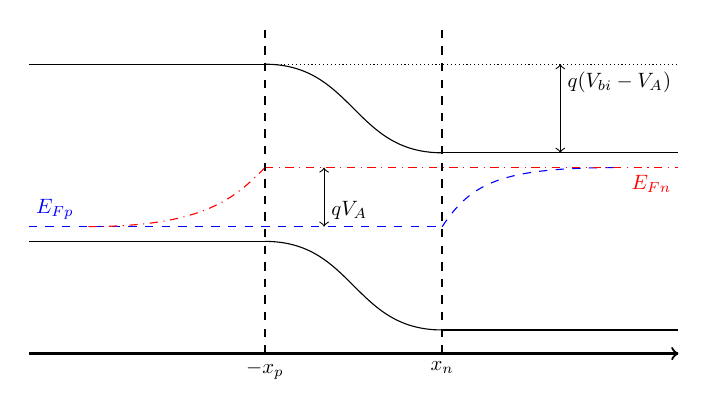
\begin{tikzpicture}[scale=0.75, transform shape]
        %disegno l'unione di due SC
        %asse x e label
        \draw[thick] (0,-1.9) --++ (4,0) node[anchor=north]{$-x_p$}--++ (3,0) node[anchor=north]{$x_n$}--++ (4,0);
        \draw[thick,->] (10.9,-1.9)--++ (0.1,0);
        %mezzo 1
        \draw(0,3) --++ (4,0);
        \draw(0,0) --++ (4,0);
        %mezzo 2
        \draw(7,1.5) --++ (4,0);
        \draw(7,-1.5) --++ (4,0);
        %livelli di fermi
        \draw[dashed,blue] (0,0.25) node[anchor=south west]{$E_{Fp}$} --++ (7,0);
        \draw[dashed, blue ] (7,0.25)..controls (7.5,1) and (8,1.25).. (10,1.25);
        
        \draw[dash dot,red] (4,1.25) --++ (7,0) node[anchor=north east]{$E_{Fn}$};
        \draw[dash dot,red] (4,1.25)..controls (3.5,0.75) and (3,0.25).. (1,0.25);
        %intersezione
        \draw[] (4,3)..controls (5.5,3) and (5.5,1.5).. (7,1.5);
        \draw[] (4,0)..controls (5.5,0) and (5.5,-1.5).. (7,-1.5);
        %delimitazioni
        \draw[thick, dashed] (4,-1.9)--++ (0,5.5);
        \draw[thick, dashed] (7,-1.9)--++ (0,5.5);
        %altro
        \draw[<->] (5,1.25)-- (5,0.25) node[anchor=south west]{$qV_A$};
        \draw[densely dotted] (4,3)--++ (7,0);
        \draw[<->] (9,3) node[anchor=north west]{$q(V_{bi}-V_A)$}-- (9,1.5);
    \end{tikzpicture}
    \caption{Caption}%
    \label{fig:enter_label}
\end{figure}
Quando il potenziale applicato $V_A \neq 0$, i livelli di fermi dei due semiconduttori non combaciano più ma sono traslati e prendono il nome di "livelli di Quasi-Fermi ($E_{fp}$ ed $E_{fn}$)". la traslazione dei i due livelli è proporzionale all'energia potenziale $qV_A$ e quindi alla tensione $V_A$.\\
Per continuare la trattazione si definiscono i seguenti parametri:
 \begin{enumerate}
     \item $p(-x_p) \approx N_A$ è la condentrazione delle lacune nel lato p, circa costante fino ai limiti della zona di svuotamento (vale anche in condizioni di non equilibrio, purchè si abbia basso livello di iniezione);
     \item $n(-x_p)$ è la concentrazione degli elettroni (portatori minoritari) nel lato p ai limiti della zona di svuotamento;
     \item $x(x_n) \approx N_D$ è la condentrazione degli elettroni nel lato n, circa costante fino ai limiti della zona di svuotamento (vale anche in condizioni di non equilibrio, purchè si abbia basso livello di iniezione);
     \item $p(x_n)$ è la concentrazione delle lacune (portatori minoritari) nel lato n ai limiti della zona di svuotamento;
 \end{enumerate}
Per calcolare il valore della concentrazione dei portatori minoritari ricordo che $n(x) \cdot p(x) =n_i^2$, allora:
 \begin{align*}
     n_0(-x_p) &= \dfrac{n_i^2}{N_A}\\
     p_0(x_n)  &= \dfrac{n_i^2}{N_D}
 \end{align*}\\
 Unendo le considerazioni fatte con l'equazione n.\ref{eqn:Vbi}, ottengo che la concentrazione dei portatori minoritari ai limiti della regione di svuotamento è legata, all'equilibrio termodinamico, alla concentrazione dei portatori maggioritari al limite opposto:
 \begin{align}
     p_0(x_n)=p_0(-x_p) \exp \left( -\dfrac{V_{bi}}{V_T} \right)\\
     n_0(-x_p)=n_0(x_n) \exp \left( -\dfrac{V_{bi}}{V_T} \right)
 \end{align}

\cleardoublepage%
\subsection{Corrente totale nella giunzione pn}
La giunzione che stiamo trattando è bipolare, cioè la corrente che si instaura è costituita sia da elettroni che da lacune. Quindi la corrente totale è formata da quattro componenti ovvero trascinamento e diffusione di elettroni + trascinamento e diffusione di lacune:
\begin{equation}
    J = J_{n,t} + J_{n,d} + J_{h,t} + J_{h,d}
\end{equation}

Ora considero 2 ipotesi principali (ed una implicita):
\begin{enumerate}
    \item Alcune delle quattro componenti sono trascurabili nel lato n o p: per bassi livelli di iniezione \textit{(e quindi per basso $\mathcal{\vec{E}}$ che si instaura) si possono trascurare le correnti di trascinamento dei portatori minoritari rispetto alle correnti di trascinamento dei portatori maggioritari.}
    \begin{psbox}[PS]
                E' importante ricordare che la corrente di trascinamento dipende dal campo elettrico. Affinchè la corrente di trascinamento dei portatori maggioritari sia maggiore di quella dei minoritari \textbf{è necessario che ci sia un minimo di campo !}. altrimenti sarebbero tutti a zero.
            \end{psbox}
    
    \item \textit{il tasso di generazione e ricombinazione nella regione svuotata è trascurabile, e quindi le densità totali di corrente di elettroni e di lacune sono costanti nella regione svuotata.}
    
    \item (implicita) la regione non svuotata è elettricamente neutra (\textbf{o quasi neutra})
            
\end{enumerate}
La regione svuotata si trova tra le coordinate ($-x_p$ e $x_n$) poichè in campo elettrico in questa regione è diversa da zero, mentre altrove vige la quasi neutralità delle cariche ($\dfrac{dQ}{dt}\approx 0$).\\
\textbf{Per la 1° ipotesi}, la corrente dei portatori minoritari (fatta di elettroni in regione p e lacune in regione n) è costituita solo da componenti diffusive.
\begin{align*}
    J_n &\approx J_{n,d} &&\text{per } x \leq -x_p \text{ (lato p) }\\
    J_h &\approx J_{h,d} &&\text{per } x \geq x_n \text{ (lato n) }
\end{align*}
\begin{citbox}
    In particolare, ai limiti della regione di carica spaziale si ha:
    \begin{align}
        J_n(-x_p)&=J_{n,d}(-x_p)\\
        J_h(x_n) &=J_{h,d}(x_n)
    \end{align}
\end{citbox}\leavevmode\newline
Quindi, nel  caso di basso campo elettrico, la corrente totale nei lati p ed n si scrive:
\begin{align*}
    J^{tot} &\approx J_{n,d} + J_h &&\text{per } x \leq -x_p \text{ (lato p) }\\
    J^{tot} &\approx J_{h,d} + J_n &&\text{per } x \geq x_n \text{ (lato n) }
\end{align*}\\
\textbf{Per la 2° ipotesi}, la corrente di elettroni (lacune) misurata al limite destro (sinistro) della regione svuotata è identica alla corrente nel limite sinistro (destro):
\begin{align*}
    J_n(x_n)&=J_n(-x_p)\\
    J_h(x_n) &=J_h(-x_p)
\end{align*}
Dall'equazione di continuità si perviene che la $J^{tot}$ è costante in tutte le sezioni indipendentemente da x, ovvero:
\begin{align*}
    \dfrac{dQ}{dt} &+\dfrac{dJ}{dx}+G-R=0 \\
    0              &+\dfrac{dJ}{dx}+0+0=0 
\end{align*}
Dato che la corrente totale $J^{tot}$ del diodo è costante sezione per sezione, posso pensare di calcolarla in un punto a mio piacere, ovvero nel punto $x_n$:
\begin{equation*}
    J^{tot}=J(x_n)=J_n(x_n)+J_h(x_n)=J_n(-x_p)+J_h(x_n)=J_{n,d}(-x_p)+J_{h,d}(x_n)
\end{equation*}
Il risultato che si ottiene è che la densità di corrente totale è funzione delle correnti di diffusione di elettroni e lacune:
\begin{equation}
    J^{tot}=J_{n,d}(-x_p)+J_{h,d}(x_n)
\end{equation}
Valutando la corrente in $-x_p$ si ottiene la stessa equazione:
\begin{equation*}
    J^{tot}=J(-x_p)=J_n(-x_p)+J_h(-x_p)=J_n(-x_p)+J_h(x_n)=J_{n,d}(-x_p)+J_{h,d}(x_n).
\end{equation*}
E quindi
\begin{equation*}
    J^{tot}=J_{n,d}(-x_p)+J_{h,d}(x_n).
\end{equation*}
Pertanto,avendo trascurato l'effetto della ricombinazione e generazione nella regione di svuotamento, \textbf{la corrente totale di una giunzione si valuta sommando le correnti di diffusione dei portatori minoritari iniettati nei due lati della giunzione ai limiti della regione di carica spaziale}.\\
%
Ora voglio calcolare analiticamente queste correnti.
%
\textbf{Concentrazione dei portatori minoritari in eccesso}\\
Per calcolare le correnti di diffusione dei portatori minoritari iniettati in $-x_p,x_n$ è necessario \textbf{stimare la concentrazione dei portatori minoritari in eccesso ai limiti della regione di svuotamento.}:
\begin{equation}
    J^{tot}=J_{n,d}(-x_p)+J_{h,d}(x_n) = qD_n \left. \dfrac{dn}{dx}\right|_{-x_p} -qD_h \left. \dfrac{dp}{dx}\right|_{x_n}
\end{equation}
da cui
\begin{equation}
    J^{TOT}= qD_n \left. \dfrac{dn'}{dx}\right|_{-x_p} -qD_h \left. \dfrac{dp'}{dx}\right|_{x_n}
\end{equation}

In presenza di una polarizzazione applicata (cioè fuori dall'equilibrio termodinamico) è possibile, almeno in basso livello di iniezione, assumenre come costanti i quasi-livelli di Fermi di elettroni e lacune nella regione di carica spaziale.

Tenendo presente che
\begin{equation}
    p \cdot n = {n_i}^2 \cdot \exp\left( \dfrac{E_{Fn} - E_{Fh}}{k_B T} \right) \quad \text{for} \quad -x_p \leq x \leq x_n
\end{equation}

 e che $E_{Fn}-E_{Fh}=qV_A$, si ottiene:
\begin{align}
    p(x_n)\cdot n(x_n)&=n_i^2 \exp\left( \dfrac{V_A}{V_T}\right)\\
    p(-x_p)\cdot n(-x_p)&=n_i^2 \exp\left( \dfrac{V_A}{V_T}\right)
\end{align}

Supposto che per basso livello di iniezioni, la concentrazione dei portatori maggioritari non vari in modo apprezzabile rispetto all'equilibrio:
\begin{align}
    n(x_n)&=N_D\\
    p(-x_p)&=N_A
\end{align}
si ricava:
\begin{align}
    p(x_n)&=\dfrac{n_i^2}{N_D} \exp\left( \dfrac{V_A}{V_T}\right)\\
    n(-x_p)&=\dfrac{n_i^2}{N_A} \exp\left( \dfrac{V_A}{V_T}\right)
\end{align}
\begin{center}
    \begin{tikzpicture}
        [circle dotted/.style={dash pattern=on .05mm off 8mm, line cap=round}]
        %disegno asse x
            \draw[->] (-5,0)--++ (10,0)
            node[anchor=west]{$x$};
            %disegno asse y
            \draw[->] (0,-1)--++ (0,5) node[anchor=south west]{$\rho_{mobile}$};
            %disegno tratteggi
            \draw[densely dotted] (-2,0)--++ (0,4);
            \draw[densely dotted] (2,0)--++ (0,4);
            %disegno grafici
            \draw[thick, red] (-5,0.5)-- (-2,0.5)  (2,0.5)-- (5,0.5);
            \draw[thick, black] (-5,3)-- (-2,3) ; 
            \draw[thick, dash dot] (2,3)-- (5,3);
            %collegamenti
            \draw[thick] (-2,3)..controls (0.5,3) and (0.5,0.5).. (5,0.55);
            \draw[thick,dashed] (-5,0.55)..controls (-0.5,0.5) and (-0.5,3).. (2,3);
            %label 
            \node at (-3.5,4)[below]{$P$};
            \node at (3.5,4)[below]{$N$};
            
            \node at (-2,0)[below]{$-x_p$};
            \node at (2,0)[below]{$x_n$};
            
            \node at (-5,3)[left]{$N_A$};
            \node at (-5,0.5)[left]{$np_0=\dfrac{n_i^2}{N_A}$};
            
            \node at (5,3)[right]{$N_D$};
            \node at (5,0.5)[right]{$pn_0=\dfrac{n_i^2}{N_D}$};

            \draw[line width = 1.5mm,circle dotted] (-2,1.05) --++ (0,0);
            \node at (-2,1.2)[left]{$n(-x_p)$};
            \draw[line width = 1.5mm,circle dotted] (2,1.05) --++ (0,0);
            \node at ((+2,1.2)[right]{$p(x_n)$};

            \draw[<->] (-1.8,0.5)-- (-1.8,1.05) node[anchor=north west]{$n'(-x_p)$};
            \draw[<->] (1.8,0.5)-- (1.8,1.05) node[anchor= north east]{$p'(x_n)$};
    \end{tikzpicture}
\end{center}

Siccome voglio calcolare la corrente che si forma a seguito dell'iniezione dei portatori in eccesso, dovrò prendere l'equazione della concentrazione totale, calcolato nel particolare punto di interesse, e sottrargliil corrispettivo $\dfrac{n_i^2}{N}$ che si avrebbe all'equilibrio fuori dalla regione di svuotamento.:

\begin{align}
    p'(x_n)&=\dfrac{n_i^2}{N_D} \left[ \exp\left( \dfrac{V_A}{V_T}\right) -1 \right]\\
    n'(-x_p)&=\dfrac{n_i^2}{N_A} \left[\exp\left( \dfrac{V_A}{V_T}\right) -1 \right]
\end{align}
\begin{psbox}[Proseguendo..]
    Da libro: Se si trascura la corrente di trascinamento dei portatori minoritari, l'evoluzione della popolazione in eccesso in funzione della posizione segue la legge studiana nel caso di portatori minoritari in eccesso dovuta a bombardamento laterale di fotoni. (trascurare la corrente di trascinamento dei portatori minoritari è equivalente a trascurare il campo elettrico nell'equazione ci dontinuità dei portatori minoritari)
\end{psbox}
La concentrazione delle lacune in eccesso nel lato n e degli elettroni nel lato p (per quanto detto nel cit.BOX sopra) segue la legge:
\begin{align}
    p'(x_n)&=\dfrac{n_i^2}{N_D} \left[ \exp\left( \dfrac{V_A}{V_T}\right) -1 \right] \cdot \exp \left[\dfrac{-x+x_n}{L_{hn}} \right]\\
    n'(-x_p)&=\dfrac{n_i^2}{N_A} \left[\exp\left( \dfrac{V_A}{V_T}\right) -1 \right]\cdot \exp \left[\dfrac{x+x_p}{L_{np}} \right]\\
\end{align}
dove $L_{hn}=\sqrt{D_h\tau_{hn}}$ è la lunghezza di diffusione delle lacune nel lato n,
$L_{np}=\sqrt{D_n\tau_{np}}$ è la lunghezza di diffusione delle lacune nel lato p,
...

\begin{center}
    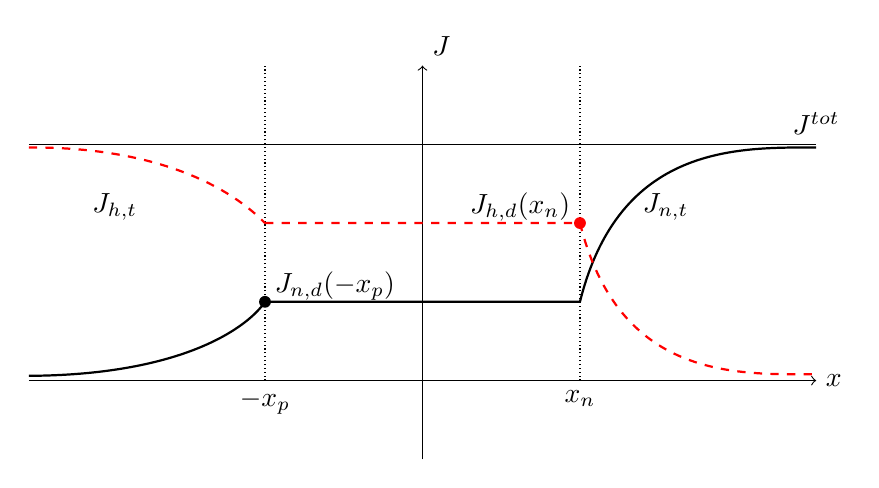
\begin{tikzpicture}
        [circle dotted/.style={dash pattern=on .05mm off 8mm, line cap=round}]
        %disegno asse x
            \draw[->] (-5,0)--++ (10,0)
            node[anchor=west]{$x$};
            %disegno asse y
            \draw[->] (0,-1)--++ (0,5) node[anchor=south west]{$J$};
            %disegno tratteggi verticali
            \draw[densely dotted] (-2,0)--++ (0,4);
            \draw[densely dotted] (2,0)--++ (0,4);
            %disegno grafici e collegamenti controls
            \draw[] (-5,3)--++ (10,0) node[anchor=south]{$J^{tot}$}; 
            \draw[thick] (-5,0.06)..controls (-3,0.07) and (-2.2,0.7).. (-2,1)
                                      (-2,1)--++ (4,0) 
                                      (2,1).. controls (2.5,3) and (4,2.96).. (5,2.96);
            \draw[thick, dashed, red]  (-5,2.96)..controls (-3,2.97) and (-2.2,2.2).. (-2,2)
                          (-2,2)--++ (4,0)   
                          (2,2).. controls (2.5,0) and (4,0.08).. (5,0.08);
            %label 
            \node at (-2,0)[below]{$-x_p$};
            \node at (2,0)[below]{$x_n$};
            
            \draw[line width = 1.5mm,circle dotted,red] (2,2) --++ (0,0);
            \draw[line width = 1.5mm,circle dotted] (-2,1) --++ (0,0);
            
            \node at (-2,1.2)[right]{$J_{n,d}(-x_p)$};
            \node at (2,2.2)[left]{$J_{h,d}(x_n)$};
            % label correnti di trascinamento portatori maggioritari
            \node at (3.5,2.2)[left]{$J_{n,t}$};
            \node at (-3.5,2.2)[left]{$J_{h,t}$};
    \end{tikzpicture}
\end{center}

La densità di corrente totale può essere ottenuta derivando rispetto ad x le concentrazioni in eccesso:
\begin{equation}
    J=\dfrac{qD_n}{L_{np}}n'(-x_p)+\dfrac{qD_h}{L{hn}}p'(x_n)
\end{equation}
ossia:
\begin{equation}
    J=qn_i^2\left( \dfrac{D_n}{N_A L{np}}+\dfrac{D_h}{N_DL{hn}} \right)\left[ \exp\left( \dfrac{V_A}{V_T}\right)-1 \right]
\end{equation}
Dove chiamo $ J_0=qn_i^2\left(\dfrac{D_n}{N_A L{np}}+\dfrac{D_h}{N_D L{hn}}\right)$ \textbf{\emph{densità di corrente inversa di saturazione}}.\\
Da notare, in realtà che l'espressione ottenuta per $J_0$ vale solo se el regioni p ed n del diodo sono lunghe rispetto alla lunghezza della diffusione ($W$).
se questo non accadesse e cioè, se la lunghezza di diffusione del lato p ($W_P$) e la lunghezza di diffusione del lato n ($W_n$) fossero paragonabili a W,la soluzione sarebbe più complessa.

per riassumere le ultime equazioni con la figura XX:
poichè il contributo della corrente di diffusione diminuisce esponenzialmente man mano che ci si allontana dal limite della regione di svuotamento, la corrente di deriva dei portatori maggioritari deve crescere in modo da mantenere costante la corrente totale

\cleardoublepage%

\section*{12/10/2023}

pg.278
\subsection{Elettrostatica della giunzione pn}
\begin{psbox}
    l'equazione di Poisson verrà risolta nella regione di svuotamento, e le dimensioni di quest'ultima ($-x_p, x_n$) verranno legate al potenziale applicato alla giunzione
\end{psbox}
Assumiamo come riferimento dell'energia potenziale il livello di Fermi intrinseco; Allora l'equazione id Poisson si scrive
\begin{equation}
    \dfrac{d^2E_{Fi}}{dx^2}=\dfrac{q\rho}{\epsilon}
\end{equation}
Lo studio che si tratterrà in seguito avrà come risultato finale le seguenti figure:\\
%
\noindent\begin{minipage}{0.6\textwidth}
    Partiamo innanzitutto considerando la densità di carica netta $\rho$:
\begin{equation}
    \rho(x) = \begin{cases}
    0&  \text{per $x < x_p$},\\
    -qN_A& \text{per $-x_p<x<0$ },\\
    qN_D& \text{per $0<x<x_n$ },\\
    0& \text{per $x>x_n$ }
\end{cases}
\end{equation}
e pertanto l'equazione di Poisson si scrive:
\begin{equation}
    \dfrac{d^2E_{F_i}}{dx^2} = \begin{cases}
    0 & \text{per $x < x_p$},\\
    -\dfrac{q^2N_A}{\epsilon}& \text{per $-x_p<x<0$ },\\
    -\dfrac{q^2N_D}{\epsilon}& \text{per $0<x<x_n$ },\\
    0 & \text{per $x>x_n$ }
\end{cases}
\end{equation}
Poichè non vi sono altre cariche presenti nel sistema, deve valere la condizione di neutralità globale \\ ($Q^+=Q^-$).\\
La carica netta totale presente deve quindi essere nulla, il che implica che nella regione di svuotamento la carica totale positiva sia pari alla carica totoale negative:
\begin{equation}
    x_n N_D=x_p N_A
\end{equation}
Per la legge di Gauss, il campo elettrico e la tensione sono legati da una relazione integrale.\\
Ricordo che il campo è nullo all'esterno della regione di svuotamento per la condizione di neutralità e quindi,  integrando una volta l'equazione di Poisson, si ottiene:
\begin{equation}
    \dfrac{dE_{F_i}}{dx} = \begin{cases}
    0 & \text{per $x < x_p$},\\
    -\dfrac{q^2N_A}{\epsilon} x + A & \text{per $-x_p<x<0$ },\\
    -\dfrac{q^2N_D}{\epsilon} x + B & \text{per $0<x<x_n$ },\\
    0 & \text{per $x>x_n$ }
\end{cases}
\end{equation}
\end{minipage}
\hfill%
\begin{minipage}{0.35\textwidth}\raggedleft
    \begin{center}
    \begin{tikzpicture}[scale=0.5]
             %disegno asse x
            \draw[->] (-5,2) node[anchor=north]{}-- (5,2)
            node[anchor=west]{$x$};
            %disegno asse y
            \draw[->] (0,-1.5)-- (0,5) node[anchor=south west]{$\rho_{fissa}(x)$};
            %disegno grafici
            \draw[thick,pattern=north east lines, pattern color=gray] (0,2)rectangle++ (4,2);
            \draw[thick,pattern=north east lines, pattern color=gray] (0,2)rectangle++ (-3,-2.5);
            %label
            \node at (4,2) [anchor=north]{$x_n$};
            \node at (-3,2) [anchor=south]{$-x_p$};
            \node at (0,4) [anchor=east]{$qN_D$};
            \node at (0,-4.5) [anchor=west]{$-qN_A$};
            \node at (2,3) [red]{$Q^+$};
            \node at (-1.5,0.75) [red]{$Q^-$};

            %disegno grafico energia
            %disegno asse x
            \draw[->] (-5,-5.5) node[anchor=north]{}-- (5,-5.5)
            node[anchor=west]{$x$};
            %disegno asse y
            \draw[->] (0,-9.5)-- (0,-3.7) node[anchor= west]{$\mathcal{E}(x)$};
            %disegno grafico rosso
            \draw[thick,red] (-5,-5.5)-- (-3,-5.5)-- (0,-9)-- (4,-5.5)-- (5,-5.5);
            %label
            \node at (0,-9) [anchor=west]{$\mathcal{E}_{MAX}$};

            %disegno grafico potenziale
            %disegno asse x
            \draw[->] (-5,-12.5) node[anchor=north]{}--++ (10,0)
            node[anchor=west]{$x$};
            %disegno asse y
            \draw[->] (0,-15.5)-- (0,-11.7) node[anchor= west]{$\phi(x)$};
            %disegno grafico rosso
            \draw[thick] (-5,-12.5)--++ (2,0).. controls (1,-12.5) and (-0,-15.7) .. (4,-15.5)--++ (1,0);
            \draw[<->] (4,-15.5)-- (4,-12.5);
            \node at (4,-14)[anchor=west]{$q(V_{bi}-V_A)$};
            %label
            \node at (0,-9) [anchor=west]{$\mathcal{E}_{MAX}$};
    \end{tikzpicture}
\end{center}
\end{minipage}


Ma il campo deve essere continuo in $x$, per cui $x=-x_p$ la derivata del livello di Fermi intrinseco si deve annullare, e così per $x=x_n$. Allora:
\begin{align*}
    -\dfrac{q^2N_A}{\epsilon} x_p + A = 0
\end{align*}
da cui:
\begin{align*}
    A = \dfrac{q^2N_A}{\epsilon} x_p
\end{align*}
    Analogamente, nel punto $x_n$:
\begin{align*}
     \dfrac{q^2N_D}{\epsilon} x_n + B =0
\end{align*}
   da cui:
\begin{align*}
     B = -\dfrac{q^2N_D}{\epsilon} x_n
\end{align*}
Questo porta alla soluzione
\begin{equation}
    \dfrac{dE_{F_i}}{dx} = \begin{cases}
    0 & \text{per $x < x_p$},\\
    -\dfrac{q^2N_A}{\epsilon} (x + x_p) & \text{per $-x_p<x<0$ },\\
    -\dfrac{q^2N_D}{\epsilon} (x - x_n ) & \text{per $0<x<x_n$ },\\
    0 & \text{per $x>x_n$ }
\end{cases}
\end{equation}

Adesso integro un'ultima volta, considerando l'equazione di neutralità globale:

\begin{equation}
    E_{F_i}= \begin{cases}
    A & \text{per $x < x_p$},\\
    -\dfrac{q^2N_A}{2\epsilon} {(x + x_p)}^2 + B& \text{per $-x_p<x<0$ },\\
    -\dfrac{q^2N_D}{2\epsilon} {(x - x_p)}^2 + C& \text{per $0<x<x_n$ },\\
    D & \text{per $x>x_n$ }
\end{cases}
\end{equation}
Ora mi servono delle condizioni a contorno. Supponiamo di assumere come riferimento dell'energia potenziale il lato sinistro della giunzione. Si ha allora:
\begin{equation}
    E_{Fi}= \begin{cases}
        0 & \text{ per $x<-x_p$},\\
        -q(V_{bi}-V_A) & \text{ per $x>x_n$}
    \end{cases}
\end{equation}
Imponendo la prima condizione si ha subito A=0.\\
La continuità dell'energia potenziale in $x=-x_p$ fornisce B=0;\\
per $x=0$ si ottiene 

\begin{align}
    E_{Fi}(0^-)=-q^2\dfrac{N_A}{2\epsilon}x_p^2 &=E_{Fi}(0^+)=q^2\dfrac{N_D}{2\epsilon}x_n^2 + C
\end{align}
da cui:
\begin{align}
    C= -q^2\dfrac{N_D}{\epsilon}x_n^2 &- q^2\dfrac{N_D}{\epsilon}_n^2 = -q(V_{bi-V_A})
\end{align}

sapendo che $\mathcal{\vec{E}}(x=0)=N_a \cdot x_p = N_D \cdot x_n$ si perviene alla profondità di diffusione:

\begin{align}
    x_n&= \sqrt{\dfrac{2\epsilon N_{eq}(V_{bi}-V_A)}{qN_D^2}}\\
    x_p&= x_n\dfrac{N_D}{N_A}= \sqrt{\dfrac{2\epsilon N_{eq}(V_{bi}-V_A)}{qN_A^2}}
\end{align}
Dove $\dfrac{1}{N_{eq}}= \dfrac{1}{N_D} + \dfrac{1}{N_A}$.\\

L'estensione totale $X_n + x_p$ della regione di svuotamento aumenta in polarizzazione inversa e diminuisce in polarizzazione diretta, fino ad annullarsi (teoricamente) per $V_A=V_{bi}$.\\
L'estensione della regione di svuotamento è tanto minore quanto maggiore è il drogaggio;
inoltre, l'estensione della regione di svuotamento nel lato meno drogato della giunzione è maggiore di quella nel lato più drogato.\\

è importante notare che il campo elettrico massimo si ha nel punto x=0:
\begin{equation}
    \mathcal{\vec{E}}_{MAX}=-q^2\dfrac{N_A}{\epsilon}x_p=-q^2\dfrac{N_D}{\epsilon}x_n
\end{equation}
\subsection{Circuito equivalente di un diodo pn}
\begin{psbox}[\small{ QUAL'E' LA DIFFERENZA TRA LA CAPACITA' DI UN CONDENSATORE E QUELLA DI UNA GIUNZIONE PN? }]
    In un normale condensatore, la capacità è creata da due piastre conduttrici separate da un materiale dielettrico. La carica è immagazzinata nel dielettrico e la capacità è determinata dalla superficie delle piastre, dalla distanza tra loro e dalle proprietà del materiale dielettrico.\\
    
    \textbf{applicare un potenziale positivo su una delle armature del condensatore provoca un accumulo di cariche positive (+q) su quest'ultima e viceversa accade per il terminale negativo.}\\
    In questo modo si crea un accumulo di cariche: + q nel lato positivo della batteria e -q nel lato negativo della batteria.
    I valori assoluti delle quantità +q e - q sono identiche identiche e vale la relazione  $C=Q/V$
    \begin{center}
        \begin{tikzpicture}[scale=0.65,transform shape]
        % condensatore
            \draw(0,0) node[anchor=east]{$+V$}-- (2,0);
            \draw(2,1) node[anchor=south]{$+q$}-- (2,-1);
            \draw(3,1) node[anchor=south]{$-q$}-- (3,-1);
            \draw(3,0)-- (5,0) node[anchor=west]{$-V$};
        \end{tikzpicture}
    \end{center}
    In un diodo a giunzione PN, la capacità si forma a causa del drogaggio che porta alla formazione della regione di svuotamento.
    A seconda del drogaggio, potro avere una regione -q a sinistra e +q a destra, o viceversa.\\ \textbf{Nel diodo il segno delle cariche non dipende dal potenziale a cui è applicato ma dal drogaggio!}. Le cariche -q e +q sono diverse in modulo e segno.
    \begin{center}
        \begin{tikzpicture}[scale=0.65,transform shape]
            % giunzione
            \draw(0,0) node[anchor=east]{$?$}-- (1.5,0);
            \draw(1.5,1) rectangle ++ (1,-2);
            \draw(2.5,1) rectangle ++ (1,-2);
            \draw(3.5,0)-- (5,0) node[anchor=west]{$?$};
            %label
            \node at (2,0) []{$Q^-$};
            \node at (3,0) []{$Q^+$};
        \end{tikzpicture}
    \end{center}
    per approfondire, quando il diodo è polarizzato inversamente la regione di svuotamento si allarga e agisce come un dielettrico con una certa capacità. La larghezza della regione di svuotamento influisce sulla capacità di giunzione. È essenzialmente una funzione della tensione applicata al diodo e delle proprietà del materiale semiconduttore.
    Nel caso del diodo, si avrà che \[ C = \dfrac{dQ}{dV_A}\]
\end{psbox}

Il diodo pn possiede, non a caso, le caratteristiche di un condensatore: è in grado di accumulare carica elettrica e, se sottoposto a sorgente variabile, il diodo pn non risponde istantaneamente ma mostra un comportamento tipico di un bipolo reattivo.\\
Nella giunzion pn si accumula carica in due regioni:
\begin{enumerate}
    \item carica fissa nella regione di svuotamento
    \item carica mobile in eccesso o in difetto nelle regioni in cui i portatori minoritari in eccesso vengono iniettati
\end{enumerate}
La carica presente nella regione di svuotamento dipende in modo istantaneo dalla tensione applicata dala giunzione, al contrario la carica iniettata in eccesso dipende dalla tensione istantanea solo per variazioni sufficientemente lente della tensione.
\cleardoublepage%

\subsubsection*{Capacità di giunzione}
La regione di svuotamento di una giunzione PN è costituita da uno strato di ioni fissi negativi nella regione drogata p, e ioni fissi negativi nella regione drogata N.
\begin{center}
    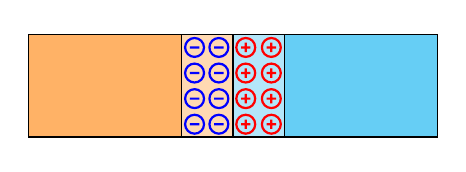
\begin{tikzpicture}[scale=0.65]
        \draw[fill=orange!60] (0,0) rectangle++ (3,2);
        \draw[fill=orange!30] (3,0) rectangle++ (1,2);
        \draw[fill=cyan!30] (4,0) rectangle++ (1,2);
        \draw[fill=cyan!60] (5,0) rectangle++ (3,2);
        %ioni negativi
        \foreach \pos in {0.25,0.75,1.25,1.75} {
        \node at (3.25,\pos) { \tikz\draw[thick,blue, scale=0.75]
        circle (0.16cm) (-0.08,0)-- (0.08,0) ;};}
        \foreach \pos in {0.25,0.75,1.25,1.75} {
        \node at (3.725,\pos) { \tikz\draw[thick,blue, scale=0.75]
        circle (0.16cm) (-0.08,0)-- (0.08,0) ;} ;}
        %ioni positivi
        \foreach \pos in {0.25,0.75,1.25,1.75} {
        \node at (4.25,\pos) { \tikz\draw[thick,red, scale=0.75]
        circle (0.16cm) (-0.08,0)-- (0.08,0) (0,0.08)-- (0,-0.08) ;} ;}
        \foreach \pos in {0.25,0.75,1.25,1.75} {
        \node at (4.75,\pos) { \tikz\draw[thick,red, scale=0.75]
        circle (0.16cm) (-0.08,0)-- (0.08,0) (0,0.08)-- (0,-0.08) ;} ;}
    \end{tikzpicture}
\end{center}

la concentrazione di questi ioni è tale per cui la carica positiva totale è uguale alla carica negativa totale.\\
Nel caso generale studiato in classe, la carica positiva è data da:
\begin{equation}
    Q_j = qAx_n N_D=|-qAx_p N_A|=A\sqrt{2q\epsilon N_{eq}(V_{bi}-V_A)}
\end{equation}
dove A è l'area della giunzione. Notiamo che l'unica variabile dell'equazione è $x_n(V_A)$.\\
La carica accumulata nella regione di svuotamento è quindi funzione istantanea della tensione applicata $V_A$; \\
E' possibile definire la capacità di giunzione associata alla caratteristica $Q_J (V_A) $ come:
\begin{equation}
    C_j=\left| \dfrac{dQ_j}{dV_A}\right|=A\sqrt{\dfrac{q\epsilon N_{eq}}{2(V_{bi}-V_A)}}
\end{equation}

\textbf{La capacità $C_J$ tende a decrescere durante la polarizzazione inversa a causa dell'allargamento della regione di carica spaziale}, mentre tende all'infinito quando la regione di carica spaziale scompare.

\begin{center}
    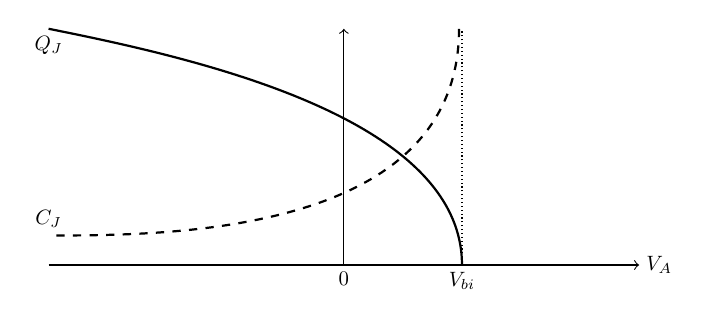
\begin{tikzpicture}[scale=0.75,transform shape]
        %disegno asse x
        \draw[->] (-5,0)--++ (10,0) node[anchor= west]{$V_A$};;
        %disegno asse x
        \draw[->] (0,0) node[anchor=north]{$0$}--++ (0,4);
        %disegno tratteggio
        \draw[densely dotted] (2,0) node[anchor=north]{$V_{bi}$}--++ (0,4);
        %disegno C_j
        \draw[thick,dashed] (1.95,4)..controls (1.95,0.5) and (-3,0.5).. (-5,0.5) node[anchor=south]{$C_J$};
        %disegno Q_j
        \draw[thick] (-5,4) node[anchor=north]{$Q_J$}..controls (-2.5,3.5) and (2,2.5).. (2,0);
    \end{tikzpicture}
\end{center}

\subsubsection*{Capacità di diffusione}
Adesso vogliamo vedere la carica mobile.\\

\begin{center}
    \begin{tikzpicture}[scale=0.9,transform shape]
        [circle dotted/.style={dash pattern=on .05mm off 8mm, line cap=round}]
        %disegno asse x
            \draw[->] (-5,0)--++ (10,0)
            node[anchor=west]{$x$};
            %disegno asse y
            \draw[->] (0,-1)--++ (0,5) node[anchor=south west]{$\rho_{mobile}$};
            %disegno tratteggi
            \draw[densely dotted] (-2,0)--++ (0,4);
            \draw[densely dotted] (2,0)--++ (0,4);
            %disegno grafici
            \draw[] (-5,0.5)-- (-2,0.5)  (2,0.5)-- (5,0.5);
            \draw[thick, black] (-5,3)-- (-1,3) ; 
            \draw[thick, dash dot] (2,3)-- (5,3);
            %collegamenti
            \draw[thick] (-1,3)..controls (1,3) and (2.5,0.55).. (5,0.55);
            \draw[thick,dashed] (-5,0.55)..controls (-0.5,0.5) and (-0.5,3).. (2,3);
            %label 
            \node at (-3.5,4)[below]{$P$};
            \node at (3.5,4)[below]{$N$};
            
            \node at (-2,0)[below]{$-x_p$};
            \node at (2,0)[below]{$x_n$};
            
            \node at (-5,3)[left]{$N_A$};
            \node at (-5,0.5)[left]{$np_0=\dfrac{n_i^2}{N_A}$};
            
            \node at (5,3)[right]{$N_D$};
            \node at (5,0.5)[right]{$pn_0=\dfrac{n_i^2}{N_D}$};

            \draw[line width = 1.5mm, dotted] (-2,1.05) --++ (0,0);
            \node at (-2,1.4)[left]{$np_0 e^{\dfrac{V_A}{V_T}}$};
            \draw[line width = 1.5mm, dotted] (2,1.65) --++ (0,0);
            \node at (+2,2)[right]{$pn_0 e^{\dfrac{V_A}{V_T}}$};

            % sottolineo area
            \draw[pattern=north east lines, pattern color=red] (-2,0.5)-- (-5,0.5)-- (-5,0.55)..controls (-2.9,0.55) and (-2,1.05).. (-2,1.05)-- (-2,0.5);

            \draw[pattern=north east lines, pattern color=red] (2,0.5)-- (5,0.5)-- (5,0.55)..controls (3.5,0.55) and (2,1.65).. (2,1.65)-- (2,0.5);
    \end{tikzpicture}
\end{center}

La presenza di portatori minoritari iniettati in eccesso in polarizzazione diretta, e di portatori minoritari in difetto in polarizzazione inversa, dà luogo ad un accumulo di carica esterno alla regione di svuotamento.\\
La carica totale in eccesso nel lato n (dovuta alle lacune iniettate dal lato p ) si scrive

\begin{equation}
    Q_n'=qA\int_{x_n}^{\infty} p'(x_n) \exp\left[ -\dfrac{x-x_n}{L_{hn}} \right] dx=qAp'(x_n)L_{hn}
\end{equation}
Mentre la carica in eccesso dovuta agli elettroni iniettati nel lato p si scrive:
\begin{equation}
    Q_p'=-qA\int_{-\infty}^{-x_p} n'(-x_p) \exp\left[ \dfrac{x+x_p}{L_{np}} \right] dx=-qAn'(-x_p)L_{np}
\end{equation}

Si noti che le cariche che si affacciano ai capi della giunzione sono diverse.\\
Introducendo la dipendenza delle concentrazioni in eccesso dalla tensione di polarizzazione si noterà che, in condizioni quasi-stazionarie, la carica in eccesso nel lato p ed n dipenderanno dalla tensione $V_A$ applicata:

\begin{equation}
    Q_n'=qA\dfrac{n_i^2}{N_D}L_{hn}\left( e^{{V_A}/{V_T}}-1\right)
\end{equation}
\begin{equation}
    Q_p'=-qA\dfrac{n_i^2}{N_A}L_{np}\left( e^{{V_A}/{V_T}}-1\right)
\end{equation}

Le espressioni precedenti valgono solo per variazioni sufficientemente lente della tensione applicata.\\
Si possono definire inoltre, le capacità differenziali quasi-statiche:
\begin{equation}
    C_{Dn}=\left| \dfrac{dQ_n'}{dV_A}\right|=\dfrac{dQ_n'}{dV_A}=\dfrac{qA}{V_T}\dfrac{N_i^2}{N_D}L_{hn}e^{\dfrac{V_A}{V_T}}
\end{equation}
\begin{equation}
    C_{Dp}=\left| \dfrac{dQ_p'}{dV_A}\right|=-\dfrac{dQ_p'}{dV_A}=\dfrac{qA}{V_T}\dfrac{N_i^2}{N_A}L_{np}e^{\dfrac{V_A}{V_T}}
\end{equation}
tutto questo lo possiamo vedere nella figura seguente.le aree che si creano a causa dell'eccesso di cariche al di fuori della regione di svuotamento, sono assimilate a condensatori in parallelo:

\begin{center}
    \begin{circuitikz}[scale=0.6, every node/.style={scale=0.75}]
        [circle dotted/.style={dash pattern=on .05mm off 8mm, line cap=round}]
        %disegno asse x
            \draw[->] (-5,0)--++ (10,0)
            node[anchor=west]{$x$};
            %disegno asse y
            \draw[->] (0,-1)--++ (0,5) node[anchor=south west]{$\rho_{mobile}$};
            %disegno tratteggi
            \draw[densely dotted] (-2,0)--++ (0,4);
            \draw[densely dotted] (2,0)--++ (0,4);
            %disegno grafici
            \draw[] (-5,0.5)-- (-2,0.5)  (2,0.5)-- (5,0.5);
            \draw[thick, black] (-5,3)-- (-1,3) ; 
            \draw[thick, dash dot] (2,3)-- (5,3);
            %collegamenti
            \draw[thick] (-1,3)..controls (1,3) and (2.5,0.55).. (5,0.55);
            \draw[thick,dashed] (-5,0.55)..controls (-0.5,0.5) and (-0.5,3).. (2,3);
            %label 
            \node at (-3.5,4)[below]{$P$};
            \node at (3.5,4)[below]{$N$};
            
            \node at (-2,0)[below]{$-x_p$};
            \node at (2,0)[below]{$x_n$};
            
            \node at (-5,3)[left]{$N_A$};
            \node at (-5,0.5)[left]{$np_0=\dfrac{n_i^2}{N_A}$};
            
            \node at (5,3)[right]{$N_D$};
            \node at (5,0.5)[right]{$pn_0=\dfrac{n_i^2}{N_D}$};

            % sottolineo area
            \draw[pattern=north east lines, pattern color=red] (-2,0.5)-- (-5,0.5)-- (-5,0.55)..controls (-2.9,0.55) and (-2,1.05).. (-2,1.05)-- (-2,0.5);
            \draw[pattern=north east lines, pattern color=red] (2,0.5)-- (5,0.5)-- (5,0.55)..controls (3.5,0.55) and (2,1.65).. (2,1.65)-- (2,0.5);
            
            %disegno circuito
            \draw(-5,-2.5) node[left]{$+V$} to [short,*-]++ (0.5,0) coordinate (a);
            \draw(a)--++ (0,1) to [C,l_=\small{$C_{Dp}$}]++ (2.5,0) 
            to [short] (4.5,-1.5)--++ (0,-1) coordinate (b);
            \draw(a)--++ (0,-1) to [short] (2,-3.5)
            to [C,l_=\small{$C_{Dn}$}] (4.5,-3.5) -| (b);
            \draw(b) to [short,-*] (5,-2.5) node[right]{$-V$};
            %disegno freccie verso il circuito
            \draw[->] (-2.3,0.7) ..controls (-3.25,0.2) and (-3.25,0).. (-3.25,-1) node[anchor=south west]{$Q'_p$};
            \draw[->] (2.3,1) ..controls (3.25,-0.5) and (3.25,-1).. (3.25,-3) node[anchor=south west]{$Q'_n$};
    \end{circuitikz}
\end{center}
Dallo schema possiamo vedere molto chiaramente come
\textbf{La capacità di diffusione è la somma delle due capacità differenziali ottenute}:
\begin{equation}
    C_D=C_{Dn}+C_{Dp}
\end{equation}
La capacità $C_D$ è elevata in polarizzazione diretta, trascurabile in polarizzazione inversa.\\
Come per la capacità di giunzione, anche la capacità di diffusione dipende dalla polarizzazione.

Il circuito equivalente finale è il seguente:

\begin{center}
    \begin{circuitikz}[scale=0.75,transform shape]
        \draw(0,0) node[anchor= west]{$\dfrac{V_A}{2}$} to [short,-o]++ (0,0) --++ (0,-0.5) coordinate (z) ;
        \draw(z)--++ (2,0) to [I>=$J(V_A)$]++ (0,-2)--++ (-2,0) to node[anchor= north west]{$-\dfrac{V_A}{2}$}++ (0,-0.5) to [short,-o]++ (0,0);
        \draw(z)--++ (-2,0) to [C,l_=\small{$C_D(V_A)$}]++ (0,-2)--++ (2,0);
        \draw(z) to [C,l_=\small{$C_J(V_A)$},*-*]++ (0,-2);
    
        % diodo
        \draw(-7,0) node[anchor= west]{$\dfrac{V_A}{2}$} to [short,-o]++ (0,0)--++ (0,-0.5)
        to [D]++ (0,-2)
        to node[anchor= north west]{$-\dfrac{V_A}{2}$}++ (0,-0.5) to [short,-o]++ (0,0);
        \draw(-5,-1.25) to [short]++ (0.5,0);
        \draw(-5,-1.5 ) to [short]++ (0.5,0);
        \draw(-5,-1.75) to [short]++ (0.5,0);
    \end{circuitikz}
\end{center}

Ora voglio andarea calcolare l'andamento della corrente.
Esiste una relazione tra la densità di diffusione e la corrente $I(V_A)$ ed è giusto che sia così, perchè queste cariche (che creano la capacità di diffusione) in eccesso nascono a causa della diffusione dei portatori minoritari. siccome però la diffusione dei portatori minoritari è anche la causa della corrente allora, necessariamente ci deve essere una relazione tra corrente e carica.
Supponiamo di avere un diodo fortemente drogato $N_D >> N_A$ deto anche diodo assimmetrico, situazione che si verifica nel caso di diodi integrati. Allora:
\begin{align}
    I_D \approx A \cdot J_{n,D}= \dfrac{AqD_nn'(-x_p)}{L_{np}}
\end{align}
?????\\
Se questa quantità la moltiplico per $\dfrac{\tau_0}{\tau_n}$.\\
La corrente di diffusione degli elettroni ai limiti della regione di svuotamento è:
min 1.22.00\\
\begin{equation}
    I_{nD}=AJ_{nD} =A\dfrac{qn'(-x_p)D_n}{L_{np}}=A\dfrac{qn'(-x_p)L_{np}}{\tau_n} \approx - \dfrac{Q'_p}{\tau_n}
\end{equation}
\begin{ricevimento}
    chiedere tutta questa parte
\end{ricevimento}
sapendo che la conduttanza differenziale del diodo è:
\begin{equation}
    g_D=\dfrac{dI}{dV_A}=\dfrac{qA}{V_T}\dfrac{n_i^2 D_n}{N_A L_n}e^{\dfrac{V_A}{V_T}}
\end{equation}
ottengo che
\begin{equation}
    C_D=\tau_nG_d
\end{equation}
Pertanto in un diodo asimmetrico la capacità di diffusione è pari al prodotto della conduttanza differenziale e della vita media dei portatori iniettati dal lato più drogato al lato meno drogato. Tale equazione può essere usata per stimare, in mancanza di ulteriori informazioni sulla struttura, la capacità di diffusione di un diodo reale.\\
Si noti che in polarizzazione diretta la conduttanza differenziale del diodo diviene molto elevata, in quanto il diodo si comporta sostanzialmente come un corto circuito; contemporaneamente però cresce anche la capacità, in modo tale che la costante di tempo RC (data dal prodotto capacità - resistenza differenziale, ossia
$C_D/G_d$) resta costante. In polarizzazione inversa la conduttanza differenziale e la capacità di diffusione divengono trascurabili, per cui la costante di tempo del sistema è dominata dalla capacità della regione di svuotamento.

\section*{16.10.2023}

\subsection{Comportamento dinamico del diodo PN}
%
\subsubsection{transitorio di chiusura OFF-ON}
Supponiamo di considerare la commutazione di un diodo che viene pilotato da un generatore di tensione a gradino che passa da un valore $-V_R$ (Vreverse) e un valore $V_F$ (Vforward).\\
Suppongo che il diodo sia inizialmente interdetto (OFF) con corrente inversa inizialmente nulla ($I_R=0$) e pertanto con tensione iniziale nulla. 

Dal punto di vista fisico, utilizzando le nozioni imparate poco prima, capisco che per tensioni sufficentemente elevate, La corrente iniettata dal generatore causa un graduale aumento della popolazione di lacune in eccesso all'interno del lato n del diodo, che inizialmente è nulla.\\
Quando il diodo è OFF, l'antamento della concentrazione Pn(x) è segnato in rosso. quando il diodo è ON si avrà un graduale incremento della concentrazione.\\

\begin{figure}[hbt!]
\centering
    \begin{circuitikz}
        % disegno asse x
        \draw[->] (-0.5,0)-- (5,0) node[right]{$x$};
        % disegno asse y
        \draw[->] (0,-0.15) node[below]{$x_n$}-- (0,2.5) node[right]{$pn(x)$};
        %disegno retta
        \draw[thick] (0,0.5)--++ (5,0) node[right]{$Pn_{0}$};
        %disegno diodo OFF
        \draw[red,thick] (0,0).. controls (1.5,0.4) and (2,0.5).. (5,0.5);
        
        %disegno altro grafici
        \draw[blue] (0,0.2).. controls (1.5,0.4) and (2,0.5).. (5,0.5);
        \draw[blue] (0,1)  to [out=320, in=180,distance=1 cm]  (5,0.5);
        \draw[blue] (0,1.75) to [out=300, in=180,distance=1.25 cm] (5,0.5);
        \begin{scope}[scale=0.75]
            %disegno tratteggi
            \draw[densely dotted] (0,0)-- (0,-2);
            \draw[densely dotted] (-1,-1)-- (-1,-2);
            \draw[densely dotted] (-1.25,-1)-- (-1.25,-2);
            %disegno giunzione
            \draw[] (-2.5,-2) rectangle (6,-1);
            \draw(-2.5,-1.5) to [R,l_=$R$]++ (-1.5,0) to [V]++ (0,-2) node[tlground]{};
            \draw(6,-1.5) to [short]++ (1.5,0) to [short]++ (0,-2) node[tlground]{};
            \node at (-1.75,-1.5)[]{$p^+$};
            \node at (3,-1.5)[]{$n$};
            %arrow
            \draw[black,-latex] (1.15,0.1) arc (200:145:2);
            \draw[-latex] (4.5,-2.5)--++ (-6,0) node[below]{$V(t)$};
        \end{scope}
    \end{circuitikz}
    \caption{Transitorio OFF-ON del pn dal punto di vista fisico}
    \label{Transitorio OFF-ON del pn dal punto di vista fisico}
\end{figure}
%

Quello che succede dal punto di vista elettrotecnico e spiegato nella seguente figura:
\begin{figure}[hbt!]
\centering
    \begin{circuitikz}[scale=.65]
        % disegno asse x
        \draw[->] (-5,0)-- (5,0) node[right]{$t$};
        % disegno asse y
        \draw[->] (0,-1.5)-- (0,4) node[right]{$I_{diodo}$};
        %disegno grafico
        \draw[thick, red] (-5,-0.5)--++ (5,0)
            --++ (0,3.5)--++ (0.7,0)
           ..controls (1.5,2) and (2,1.5).. (5,1.5);
        % tratteggi
        \draw[dashed] (0,1.5)--++ (5,0);
        %disegno aperture per spazio circuiti
        \draw[densely dotted] (0,-1.5) -- (-3.3,-2)--++ (0,-3);
        \draw[densely dotted] (0.7,3)--++ (0,-4.5) -- (4,-2)--++ (0,-3);
        %label
        \node at (0,-0.5) [right]{$-I_R$};
        \node at (0,3) [left]{$\dfrac{V_F+V_R}{R}$};
        \node at (0,1.5) [left]{$\dfrac{V_F}{R}$};
        
        %disegno grafico sinistra
        \draw(-6.7,-6) coordinate (zero)
        to [short]++ (-1.5,0)
        to [sqV,v<=$-V_R$]++ (0,2)
        to [R, l=$R$] ++ (3,0)
        to [D, v^<=$V_R$]++ (0,-2)
        to [short,-*]++ (-1.5,0)
        node[ground]{}++ (0,-0.1);
        %disegno grafico centrale
        \draw(0.35,-6) coordinate (zero)
        to [short]++ (-1.5,0)
        to [sqV,v<=$V_{A}$]++ (0,2)
        to [R, l=$R$] ++ (3,0)
        to [C, v^<=$V_R$]++ (0,-2)
        to [short,-*]++ (-1.5,0)
        node[ground]{}++ (0,-0.1);
        %disegno grafico denstra
        \draw(7.7,-6) coordinate (zero)
        to [short]++ (-1.5,0)
        to [sqV,v<=$V_F$]++ (0,2)
        to [R, l=$R$] ++ (3,0) coordinate (x)
        to [D, v^=$V_F$]++ (0,-2)
        to [short,-*]++ (-1.5,0)
        node[ground]{}++ (0,-0.1);
        \draw(x) --++ (0,-2);
    \end{circuitikz}
    \caption{Transitorio OFF-ON del pn dal punto di vista elettronico}
    \label{Transitorio OFF-ON del pn dal punto di vista elettronico}
\end{figure}\\
%
\cleardoublepage%
\textbf{Analisi della commutazione:}\\
Per $t=0^-$ la tensione ai capi del diodo è pari a $-V_R$ e la corrente del diodo è virtualmente nulla ($I_{diodo}=I_R=-I_0$ dove $I_0$ è la corrente di diffusione degli elettroni dal lato p al lato n e di lacune dal lato n al lato p).\\

cosa succede per $t=0^+$?\\
A causa della capacità parallela del diodo, la tensioni ai capi del diodo non può commutare istantaneamente, per cui per $t=0^+$ la tensione ai capi del diodo è ancora $-V_R$ .\\
Pertanto la corrente che fluisce nel diodo per $t=0^+$ è una corrente diretta?? pari a:
\begin{equation}
    I_F(0^+) \approx \dfrac{V_F - (-V_R)}{R}=\dfrac{V_F + V_R}{R}
\end{equation}
Questo valore è mentenuto finchè la capacità non si scarica facendo entrare il diodo in zona di conduzione.\\

mentre la corrente che fluisce in situazione di regime sarà:
%
\begin{equation}
    I_F \approx \dfrac{V_F}{R}
\end{equation}
%
Come mostrato nella figura XX, negli istanti del transitorio di chiusura il diodo presenta un overshoot di corrente rispetto al valore finale, ossia porta una corrente maggiore di quella finale.
Questo fatto non ha conseguenze rilevanti se non quello di rendere più veloce il transitorio (perchè aumenta la quantità di carica iniettata nell'unità di tempo)\\
E' importante notare che un diodo pilotato in tensione commuta in modo virtualmente istantaneo dallo stato OFF allo stato ON, ossia passa isntantaneamente da una corrnte quasi nulla ad una corrente positiva. Si può ritenere quindi che in commutazione diretta il diodo si comporti in modo praticamente ideale.


\subsubsection{transitorio di apertura ON-OFF}
Il transitorio di spegnimento (ON-OFF) risulta più complesso rispetto alla chiusura e il transitorio che ne deriva sarà fortemente non ideale ma in sostanza si basa sempre sul fatto che la tensione ai capi del diodo non può commutare istantaneamente.
%
Supponiamo di considerare la commutazione di un diodo che viene pilotato da un generatore di tensione ad onda quadra che passa da un valore $V_F$ and un valore $-V_R$.\\
\begin{figure}[hbt!]
    \centering
    \begin{circuitikz}[scale=0.75]
        % disegno asse x
        \draw[->] (-1,0)-- (6,0) node[right]{$x$};
        % disegno asse y
        \draw[->] (0,-0.5)-- (0,4) node[right]{$pn(x)$};
        %disegno retta
        \draw[thick] (0,0.5)--++ (6,0) node[right]{$pn_{0}$};
        %disegno diodo OFF
        \draw[red] (0,0)..controls (1.5,0.4) and (2,0.45).. (6,0.45);
        %disegno altri grafici blue
        \draw[blue] (0,3)..controls (1,2.25) and (2,1).. (5,0.55);
        \draw[blue] (0,2) to [out=60, in=180,distance=1cm] (3.5,0.55);
        \draw[blue] (0,1.5) to [out=15, in=180,distance=1.1cm] (2.75,0.55)--++ (3,0);
        \draw[blue] (0,0.5) to [out=70, in=180,distance=1cm] (2,0.55)--++ (4,0);

        %label
        \draw[fill=blue] (0,3) circle(2pt) node[left]{$pn_{0}e^{\frac{V_A}{V_T}}$};
        %disegno tratteggi
        \draw[densely dotted] (0,0)-- (0,-2);
        \draw[densely dotted] (-1,0)-- (-1,-2);
        \draw[densely dotted] (-1.25,-1)-- (-1.25,-2);
        %disegno giunzione
            \draw[] (-2.5,-2) rectangle (6,-1);
            \draw(-2.5,-1.5) to [R,l_=$R$]++ (-1.5,0) to [V]++ (0,-2) node[tlground]{};
            \draw(6,-1.5) to [short]++ (1.5,0) to [short]++ (0,-2) node[tlground]{};
            \node at (-1.75,-1.5)[]{$p^+$};
            \node at (3,-1.5)[]{$n$};
            %arrow
            \draw[black,latex-] (1.15,0.1) arc (200:145:2);
            \draw[-latex] (4.5,-2.5)--++ (-6,0) node[below]{$V(t)$};
    \end{circuitikz}
    \caption{Transitorio ON\_OFF del pn dal punto di vista fisico}%
    \label{fig:Transitorio_ON_OFF_del_pn_dal_punto_di_vista_fisico}
\end{figure}

durante la fase di conduzione inversa, i portatori in eccesso esauriscono con un andamento come in figura. fino a $I_i$ la concentrazione in eccesso resta maggiore di zero e la corrente è inversa mentre nelal fase compresa tra $T_I$ e $t_{I+II}$ si riduce fino a circa $I_0$
\begin{center}
    \begin{tikzpicture}[scale=0.45]
             %disegno asse x
            \draw[->] (-5,0) node[anchor=north]{}-- (5,0)
            node[anchor=west]{$t$};
            %disegno asse y
            \draw[->] (0,-3.5)-- (0,3) node[anchor=south west]{$V_A$};
            %disegno onda quadra
            \draw[thick] (-5,+2)--++ (5,0)
                 --++ (0,-4)--++ (5,0);
    \end{tikzpicture}
\end{center}

\begin{figure}[hbt!]
\centering
    \begin{tikzpicture}[scale=0.55]
    %disegno grafico tensione
        %disegno asse x
        \draw[->] (-4,0+4) node[anchor=north]{}-- (6,0+4)
        node[anchor=west]{$t$};
        %disegno asse y
        \draw[->] (0,-2.5+4)-- (0,2+4) node[anchor= west]{$V_{diodo}$};
        %disegno grafico rosso
        \draw[thick,red] (-4,1+4)-- (0,1+4); 
        \draw[thick,red] (0,1+4) to [out=0, in=90,distance=0.7cm] (2,4) node[above]{$t_1$} ;
        \draw[thick,red] (2,0+4) to [out=280, in=180] (4,-2+4)--++ (1,0);
        %label tempo
        \draw[dashed] (5,2)-- (5,4) node[above]{$t_1+t_2=t_r$};
       %disegno grafico corrente
        %disegno asse x
        \draw[->] (-4,0) node[anchor=north]{}--++ (11,0);
        node[anchor=west]{$t$};
        %disegno asse y
        \draw[->] (0,-3)-- (0,1.5) node[anchor= west]{$I$};
        %disegno grafico rosso
        \draw[thick,red] (-4,0.5)-- (0,0.5) --++ (0,-3)--++ (2,0)
       ..controls (2+1,-0.15) and (4+1,-0).. (5+1,-0);

        %disegno aperture per spazio circuiti
        \draw[densely dotted] (0,-3) -- (-3.3,-3.5)--++ (0,-3);
        \draw[densely dotted] (1+1,0.5)--++ (0,-3.5) -- (4+1,-3.5)--++ (0,-3);
        %label
        \node at (0,-0.5) [right]{$-I_R$};
        \node at (0,1.5) [left]{$\dfrac{V_F}{R}$};
        
        %disegno grafico sinistra
        \draw(-6.7,-6.5) coordinate (zero)
        to [short]++ (-1.5,0)
        to [sqV,v<=$-V_R$]++ (0,2)
        to [R, l=$R$] ++ (3,0)
        to [D, v^<=$V_R$]++ (0,-2)
        to [short,-*]++ (-1.5,0)
        node[ground]{}++ (0,-0.1);
        %disegno grafico centrale
        \draw(0.35+0.75,-6.5) coordinate (zero)
        to [short]++ (-1.5,0)
        to [sqV,v<=$V_{A}$]++ (0,2)
        to [R, l=$R$] ++ (3,0)
        to [C, v^<=$V_R$]++ (0,-2)
        to [short,-*]++ (-1.5,0)
        node[ground]{}++ (0,-0.1);
        %disegno grafico denstra
        \draw(7.7+0.75,-6.5) coordinate (zero)
        to [short]++ (-1.5,0)
        to [sqV,v<=$V_F$]++ (0,2)
        to [R, l=$R$] ++ (3,0) coordinate (x)
        to [D, v^=$V_F$]++ (0,-2)
        to [short,-*]++ (-1.5,0)
        node[ground]{}++ (0,-0.1);
        \draw(x) --++ (0,-2);
    \end{tikzpicture}
    \caption{Transitorio ON-OFF del pn dal punto di vista elettronico}
    \label{Transitorio ON_OFF del pn dal punto di vista elettronico}
\end{figure}
Se si trascura la caduta di tensione del diodo in polarizzazione diretta, si ha che la corrente del diodo subito prima della commutazione vale:
\begin{equation}
    I_F \approx \dfrac{V_F}{R}
\end{equation}
Come nel caso precedente,la tensione di giunzione del diodo non può commutare istantaneamente a causa della capacità di giunzione. Quindi per $t=0^+$ $V_j \approx 0$ e quindi:
\begin{equation}
    i(0^+) \approx \dfrac{-V_R}{R} 
\end{equation}
ossia il diodo conduce nella direzione inversa.\\
Negli istanti iniziali della commutazione, il diodo non è ingrado di comportarsi come circuito aperto, bloccando il passaggio della corrente inversa, ma si comporta come un cortocircuito.\\
Il passaggio della corrente inversa è indispensabile per eliminare i portatori in eccesso accumulati nel lato n della giunzione.\\
E' importante notare che la tensione del diodo resta positiva fino a che non si annulla, in $x_n$, la densità in eccesso delle lacune iniettate. Dopo tale istante il diodo comincia ad essere polarizzato inversamente e la corrente si riduce fino al valore asintotico $I_0$.\\
La fase di commutazione si può studiare in due parti
\begin{enumerate}
    \item La fase iniziale da $0^+$ a $t_1$ il diodo lavora a corrente costante pari a $i(0^+) \approx \dfrac{-V_R}{R}=-I_R$
$T_1$ è definito come il tempo necessario a riassorbire l'eccesso di carica.
    \item Nella fase da $t_2$ a $t_1+t_2$ la corrente del diodo si riduce ad un valore considerato trascurabile.
\end{enumerate}
Il tempo $t_1+t_2$ è definito come tempo di recovery ed è il tempo necessario a produrre l'eccesso di portatori in modalità reverse 
\begin{exbox}[approfondimento formule dal libro]
    nell'ipotesi di diodo assimmetrico $p^+n$:
     \begin{center}
         $i=\dfrac{dq_n'}{dt}+\dfrac{q_n'}{\tau_h}$
     \end{center}
    Con $i=I_F$ per $t<0$ ed $i=-I_R$ per $t>0$.\\
    La soluzione valoda per $t<t_1$, si può scrivere come:
    \begin{equation}
        q_n'(t)=\tau_h \left[ -I_R + (I_F+I_R)e^{-t/\tau_h} \right]
    \end{equation}
\end{exbox}
Nel caso delle lacune, supponendo che la carica in eccesso si annulli per $t=t_r$ si trova:
\begin{equation}
    t_r \approx \tau_h \log\left( 1 + \dfrac{I_F}{I_R}\right)
\end{equation}
Dove, per fini pratici si è posto $t_r=t_1+t_2$ mentre $\tau_h$ è il tempo di vita medio delle lacune.\\
Dall'equazione posso capire che aumentando $I_F$ si andrà ad incrementare la quantità di carica che dovrà essere svuotata. Ma a ben pensarci, l'effetto può essere bilanciato da una sufficente $I_R$ ma questo dipende dalle caratteristiche del diodo.\\
I diodi più veloci sono quelli la cui carica per diffusione è piccola, viceversa sono più lenti.\\
L'altro parametro importante è il tempo di vita medio. Per mantenere tempo di vita basso e quindi favorire la ricombinazione, si usano degli elementi (detti) contaminanti nel silicio. Atomi come l'oro creano dei livelli energetici intermedi, cioè trappole energetiche, che in commutazione aumenta il fattore di ricombinazione di elettroni e lacune.

in conclusione:
\begin{enumerate}
    \item il diodo presenta un comportamento praticamente ideale nella fase di TURN-ON
    
    \item il diodo presenta un comportamento NON ideale nella fase di TURN-OFF

    \item i diodi più veloci non hanno grosso accumulo di $Q_{DIFFUSIVA}$  
    
    \item il tempo di ritardo è proporzionalealla vita media dei portatori minoritari e dipende anche dal rapporto delle correnti diretta e inversa subito dopo la commutazione.

    \item la commutazione può essere accellerata aumentando la corrente inversa (e quindi polarizzando con una $V_A$ maggiore) ma soprattutto riducendo il tempo di vita medio dei portatori minoritari.
    Questo può essere ottenuto mediante drogaggio, introducendo livelli energetici intermedi che.....
    in genere si contamina con l'oro
\end{enumerate}
%
\cleardoublepage%
%
\subsubsection{Giunzione a polarizzazione inversa elevata}
Se la giunzione pn è sottoposta ad una polarizzazion inversa elevata, essa non si comporta come nel caso ideale.
Quello che succede è che, ad una certa tensione, il diodo subisce un processo di rottura (\textbf{\emph{BREAKDOWN: $V_{br}$}}) e la corrente aumenta bruscamente.\\
In parole povere, se viene superata la tensione inversa $V_{br}$, il diodo non è più in grado di opporsi al passaggio di corrente e si comporta come cortocircuito.

\begin{center}
    \begin{tikzpicture}[line cap=round, scale =0.85]
		%diseggno asse x
		\draw[->] (-5,0) -- (5,0) node[below] {$V_A$};
        %disegno asse y
		\draw[->] (0,-5) -- (0,5) node[left] {$I$};
		
		% plot per Va positive
		\draw[domain=-3.4:0.75, samples=400, variable=\x, very thick] plot ({0.6*\x+2},{e^(\x*2)});
		\draw[dashed, line width=0.15mm] (2.5,0) node[below] {$V_\text{s}$} --++ (0,4) ;
  
        % plot per Va negative
        \draw(0,0)-- (-0.25,-0.125)--++ (-2.5,0)
        [domain=-7:0.75, samples=400, variable=\x, very thick] plot ({-1*0.2*\x-4},{-e^(\x*2)-0.125});
		\draw[dashed, line width=0.15mm] (-4.1,0) node[] {$V_\text{br}$} --++ (0,-4) ;
	\end{tikzpicture}
\end{center} 

Ci sono tre meccanismi principali che causano la rottura del diodo, ma noi analizziamo sono i primi due:
\begin{enumerate}
    \item Rottura dovuta a moltiplicazione a valanga

    \item Rottura dovuta a effetto tunnel, più conosciuto come "effetto Zener"

    \item Rottura dovuta a perforazione diretta
\end{enumerate}
Gli effetti li studio separatamente ma bisogna sempre ricordare che nei diodi reali il meccanismo di rottura è una combinazione di tutti i meccanismi elencati.
Più avanti si vedrò che i due meccanismi hanno un diverso comportamento in temperatura.

\cleardoublepage%

\subsubsection{Rottura per perforazione diretta}
accade quando la tensione inversa provoca un aumento della regione di svuotamento talmente grande da coprire tutto il semiconduttore fino a toccare le metallizzazioni, a quel punto non c'è più resitenza al passaggio di elettroni da P verso N, anzi, vengono spinti subito dal campo elettrico dello svuotamento che ormai ricopre praticamente tutto il diodo (o la zona drogata maggiormente).

\subsubsection{Effetto Zener (o tunnel)}
%
\begin{ripasso}[RIPASSO PRIMA DI CONTINUARE]
    Nel caso di un semiconduttore di tipo p fortemente drogato, il livello di Fermi si sposterà in modo che si trovi più vicino alla banda di valenza, facilitando il movimento delle lacune e aumentando la conducibilità del materiale.\\
    Nel caso di un semiconduttore di tipo n fortemente drogato, il livello di Fermi si sposterà in modo che si trovi più vicino alla banda di conduzione, facilitando il movimento degli elettroni e aumentando la conducibilità del materiale.\\
    Siccome i due semiconduttori sono messi a contatto, per mantenere l'uniformità  del disegno, succede che le bande del P salgono in alto mentre le bande dell'N scendono provocando un assottigliamento della regione svuotata (vedi figura sotto).
\end{ripasso}
%
 Nei semiconduttori, l'effetto tunnel può verificarsi quando una particella, come un elettrone, attraversa una barriera di potenziale che teoricamente dovrebbe essere troppo alta da permetterlo. Tuttavia, a livello quantistico, esiste una probabilità non nulla che la particella possa attraversare la barriera anche se, dal punto di vista di fisica classica, non ha energia sufficiente.\\
 
Tralasciando però la probabilità quantistica, esiste un'altro caso in cui si verifica tale evento, ovvero quando i semiconduttori sono fortemente drogati al punto da abbassare i livelli di fermi sotto le regioni proibite.
Infatti, nelle giunzioni fortemente drogate la regione di svuotamente può diventare talmente sottile da permettere il passaggio di portatori dalla banda di valenza del SC1 alla banda di conduzione del SC2 attraverso la banda proibita per effetto tunnel.\\

Il flusso di portatori dovuti all'effetto tunnel aumenta con la polarizzazione inversa perchè al crescere della polarizzazione vi sono più stati pieni della banda di valenza affacciati a stati vuoti della banda di conduzione nel lato opposto alla giunzione.

Ricordo che lo spessore della regione di svuotamento vale:
%
\begin{equation}
    x_n= \sqrt{\dfrac{2\epsilon N_{eq}(V_{bi}-V_A)}{N_D^2}}
\end{equation}
%
Se $N_D \uparrow$ allora la regione si stringe molto fino a che non viene perforata (perforazione diretta). In tal caso si verifica una scarica di elettroni che passa dall'altra parte. (le correnti escono dal catodo, costituito dal mezzo drogato n).

\begin{center}
    \begin{circuitikz}[scale=0.55,transform shape]
        %disegno l'unione di due SC
        %mezzo 1
        \draw(0,3) --++ (4,0);
        \draw(0,0) --++ (4,0);
        %mezzo 2
        \draw(7,-1.5) --++ (4,0);
        \draw(7,-4.5) --++ (4,0);
        %intersezione
        \draw[] (4,3)..controls (5.5,3) and (5.5,-1.5).. (7,-1.5);
        \draw[] (4,0)..controls (5.5,0) and (5.5,-4.5).. (7,-4.5);
        % elettroni
        \foreach \pos in {2,3} {
        \node at (0.7+\pos,-0.75) { \tikz\draw[thick,fill=Ecolour]
        circle (0.14cm) (-0.07,0)-- (0.07,0) ;} ;}
        \foreach \pos in {2.5,3.5} {
        \node at (0.7+\pos,-1) { \tikz\draw[thick,fill=Ecolour]
        circle (0.14cm) (-0.07,0)-- (0.07,0) ;} ;}
        %livelli energetici
        \draw[thick,blue] (7,-0.5)--++ (2,0);
        \draw[thick,blue] (7,-1)--++ (2,0);
        %frecce da elettroni a livelli energetici
        \draw[latex-,red] (6.3,-0.45) arc(55:130:1.55);
        \draw[latex-,red] (6.4,-0.65) arc(55:130:1.53);
        %disegno batteria
        \draw(11.5,-3) to [short,*-]++ (1,0)--++ (0,-3)--++ (-7,0);
        \draw(5.5,-6) to [battery1]++ (-1,0);
        \draw(-0.5,1.5) to [short,*-]++ (-1,0)--++ (0,-7.5)--++ (+6,0);
        %label
        \node at (2,3.5) {$p$};
        \node at (9,3.5) {$n$};

        %inserisco circuito zener
        \draw(12,-0.4)--++ (0.5,0);
        \draw(12,-0.5)--++ (0.5,0);
        \draw(12,-0.6)--++ (0.5,0);

        \draw(14,-1.5) 
        to [short]++ (0,2)
        to [zDo]++ (3,0)
        to [short]++ (0,-2)
        to [battery1]++ (-3,0);
        \draw[-latex] (16,1.2)--++ (-1,0);
    \end{circuitikz}
\end{center}

L'effetto di rottura può comportare la distruzione del dispositivo, ma se viene controllato, si può utilizzare nel diodo Zener.\\

\begin{exbox}[ricordo il diodo zener]
%
Il diodo Zener viene utilizzato comé stabilizzatore di tensione nell'intorno della tensione di breakdown e non a caso  è sempre usato in polarizzazione inversa proprio perchè sfrutta il fenomeno di rottura di tipo tunnel.
\begin{center}
    \begin{circuitikz}
        \draw(0,0) node[ground]{} coordinate(gnd);
        \draw(gnd) to [short,*-]++ (-2,0)
                            to [battery2,invert, l=$V_g$]++ (0,1.5) 
                            to [R,l=$R_g$]++ (2,0) coordinate (d)
                            to [short,*-]++ (1,0)
                            to [R,l=$R_{out}$] ++ (0,-1.5)-| (gnd);
         \draw(d) to [zD,invert] (gnd);
    \end{circuitikz}
    \end{center}
    %
Quando la tensione $V_g$ supera la soglia di breakdown dello zener ($V_{br}$)  l'effetto tunner prevale, lo zener diventa praticamente un cortocircuito e fà passare una parte della corrente di $R_g$ verso massa e salvando il carico a cui è collegato.
%
\begin{align*}
    Iout=I_g-I_z
\end{align*}
%
Lo zener ha comunque dei limiti sulla quantità di corrente che può sopportare. \\
Se $I_z$  supera la soglia indicata dal progettista, il dispositivo si rompe. \\
Ulteriori osservazioni sono fatti nel capitolo xx

\end{exbox}

\subsubsection{Effetto valanga}
In presenza di campi elevati, i portatori di carica (che sono mobili) riescono ad acquisire energia sufficiente da provocare la generazione di una coppia elettrone-lacuna dopo una collisione tra atomi e impurità nel reticolo cristallino.

Le coppie elettrone lacuna ed i portatori di carica da cui sono originati vengono nuovamente accelerati dal campo elettrico ed andranno ad urtare atomi del materiale facendoli ionizzare, cioè  producendo ulteriori coppie libere (questo processo è chiamato ionizzazione da impatto) dando vita al fenomeno di moltiplicazione a valanga dei portatori che darà origine ad una forte corrente inversa.

In una giunzione pn vi sono campi intensi solo nella regione di svuotamento e quindi l'effetto valanga potrà verificarsi solo all'interno di questa regione.

\begin{psbox}
Se il campo elettrico non è sufficientemente intenso, la velocità degli elettroni non è sufficiente a mantenere il breakdown a valanga, negli urti gli elettroni sono riassorbiti dagli atomi ed il processo cessa;
\end{psbox}
\begin{figure}[hbt!]
    \centering
    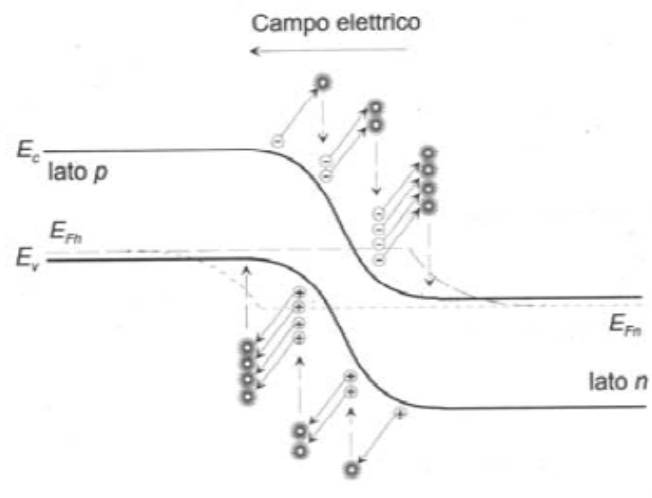
\includegraphics[width=0.5\textwidth]{Immagini_Micro&Nano/Imm_2_Fisica_dei_semiconduttori/Effetto valanga.png}
    \caption{Caption}%
    \label{fig:enter_label}
\end{figure}
%
\textbf{descrizione rigorosa:}\\
La moltiplicazione a valanga di portatori è conseguenza tipica 
 della presenza di un elevato campo elettrico. Infatti, maggiore è il campo, maggiore è la probabilità che si verichi la ionizzazione da impatto e quindi l'effetto valanga, con il conseguente aumento della corrente di trascinamento.\\
Considero un sistema monodimensionale e stazionario nel tempo: un semiconduttore di lunghezza W sottoposto ad un campo elettrico $\mathcal{E}$ (non necessariamente costante lungo x) e quindi percorso da una corrente totale di elettroni $J_n$ e di lacune $J_h$.\\
%
Suppongo  inoltre che il campo sia intenso a tal punto da rendere dominante il fenomeno di generazione per ionizzazione da impatto rispetto ad altri meccanismi, allora scrivo l'equazione di continuità in condizioni stazionarie:

\begin{align}
    \dfrac{dJ_n}{dx}&=-\alpha_h \cdot J_h - \alpha_n \cdot J_n\\
    \dfrac{dJ_h}{dx}&=\alpha_h \cdot J_h + \alpha_n \cdot J_n
\end{align}
dove $\alpha_n$ ed $\alpha_h$ sono i coefficienti di ionizzazione di elettroni e lacune; $\alpha_n$ determina quante coppie elettrone-lacuna vengono generate a causa della della distribuzione $J_n$.  analogo per $\alpha_h$.\\
%
Io sò che la corrente $J^{tot} = J_n(x) + J_h(x)$ è costante lungo $x$ perchè la corrente è uguale sezione per sezione. riscrivo l'equazione EDO nell'incognita $J_h$ usando la  $J^{tot}$ precendente ed ottengo:
%
\begin{equation}
    \dfrac{dJ_h}{dx}=\alpha_h \cdot J_h + \alpha_n \cdot (J-J_h)
\end{equation}
%
Per risolvere questa EDO mi serviranno le condizioni al contorno.
Supponiamo che il campo elettrico sia tale da rendere $J_h$ e $J_n$ positive nelle equazioni di continuità sopra scritte, allora la derivata di $J_h$ rispetto ad x è positiva, ossia $J_h$ cresce progressivamente da x=0 a x=W, 
ricordo però che $J_n=J^{tot}-J_h$ quindi, la densità di corrente di elettroni decresce per x crescenti ( analogamente cresce per x decrescenti). Questo corrsiponde al fatto che le lacune si muovano da sinistra verso destra, generando coppie elett-lacuna, mentre gli elettroni si muovono nel verso opposto.\\
%
\begin{figure}[hbt!]
    \centering
    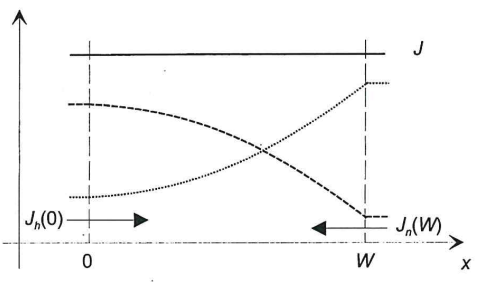
\includegraphics{Immagini_Micro&Nano/Imm_2_Fisica_dei_semiconduttori/condizioni al contorno per generazione a valanga.png}
    \caption{Caption}%
    \label{fig:enter_label}
\end{figure}
%
Per le condizioni al contorno posso, allora considera una corrente di lacune $J_h(0)$ incidente da sinistra ed una corrente di elettroni $J_n(0)$ incidente da destra. Questa considerazione non è tirata a caso infatti, posso considerarla coerente con il processo di generazione a valanga delle lacune che origina in x=0 e prosegue verso sinistra, mentre il processo per gli elettroni ha origine in x=W e procede verso destra.

La soluzione finale sarà:
%
\begin{equation*}
    J=\dfrac{\exp{\left[ \alpha_h - \alpha_n\right]_{0}^{W}} J_h(0)+J_n(W)}{\exp{\left[ \int_{0}^{W} \alpha_h - \alpha_n dx \right] \int_{0}^{W} \alpha_n \cdot \exp{\left[ -\int_{0}^{\xi} \alpha_h \alpha_n d\xi\right] dx}}}
\end{equation*}
%
l'equazione risolutiva $J$ è un qualcosa di molto complicato che non studio, tuttavia è molto importante sapere che \textbf{in presenza di una finita corrente iniettata di elettroni e lacune, la corrente totale $J$ può diventare infinita (o grande) grazie al venomeno di generazione elettrone-lacuna}.\\

A me interessa il caso particolare in cui $J \rightarrow \infty$ e questo succede solo se:
\begin{equation*}
    \int_{0}^{W}\alpha_h \exp{\left[ -\int_{0}^{x} (\alpha_h - \alpha_n) d\xi \right] dx} =1
\end{equation*}
%
l'equazione precedente è chiamata integrale di ionizzazione.\\
Per non complicare la trattazione supponiamo valide due ipotesi 
semplificative:
 \begin{enumerate}
     \item la giunzione è brusca asimmetrica ($p^+n$)
     \item I coefficienti di ionizzazione di elettroni e lacune sono uguali, ossia $\alpha_n=\alpha_h=\alpha$
 \end{enumerate}
L'integrale diventa semplice nel caso in cui si applichi la condizione semplificativa num.2.  Allora la condizione di rottura per effetto valanga diventa:
\begin{equation}
    \int_{0}^{W}\alpha_h dx = \int_{0}^{W}\alpha_n dx = 1 
\end{equation}

La condizione $\alpha_h \approx \alpha_n$ è verificata nel GaAs ed in altri semiconduttori ma non è vera nel silicio. in quest'ultimo, i due tassi di ionizzazione sono molto differenti e la condizione di valanga si ottiene per tensioni molto maggiori siccome uno dei due portatori dovrà compensare la minore efficienza di ionizzazione dell'altro.\\
%
Sia $\alpha_n$ che $\alpha_h$ sono funzioni del campo elettrico, quindi 
\begin{equation}
    \alpha_n = \alpha_h=\alpha^{\infty} \exp\left[ -\dfrac{\mathcal{E}^{crit}}{\mathcal{E}} \right]
\end{equation}

Se il campo $\mathcal{E}$ è è molto debole allora $\alpha_n=\alpha_h=0$ quindi l'integrale sopra farà 0 e la condizione "$=1$" non è mai soddisfatta.\\
Se il campo $\mathcal{E}$ è molto grande allora $\alpha_n=\alpha_h=\alpha^{\infty}$ \\
in tutte le altre condizioni, siccome il campo elettrico cambia all'interno della regione svuotata,  allora $\alpha_n$ ed $\alpha_h$ avranno certi andamenti (che noi non vediamo) e se capito che $\int_{0}^{\infty}\cdot=1$ allora si sviluppa quella corrente.\\
ricordo che il campo elettrico è pari a 
\begin{equation}
    \mathcal{E}=\mathcal{E}_{max}\ \exp\left[\dfrac{x-x_n}{x_n}\right]
\end{equation}
\textbf{CONTROLLARE FORMULA SE CORRETTA}\\
\cleardoublepage%
In definitiva ci sono due casi in cui si può verificare uno scorrere della corrente:
\begin{itemize}
    \item nel caso di effetto tunnel. nel quale c'è bisogno di un elevato drogaggio
    \item nel caso di effetto valanga nel quale c'è bisogno di un drogaggio sufficiente ma tanta $V_A$.
\end{itemize}
%
Definisco ora la tensione di breackdown in funzione del drogaggio:\\
\begin{figure}[hbt!]
    \centering
    \begin{tikzpicture}
        %disegno asse x e label
        \draw[-latex] (0,0)-- (6,0) node [right]{$\text{Drogaggio lato n }(cm^{-3}$};
        \node at (0.25,0)[below]{$10^4$};
        \node at (5.5,0)[below]{$10^{18}$};
        %disegno asse y
        \draw[-latex] (0,0)-- (0,4) node [right]{$V_{BD}$};
        \node at (0,0)[left]{$1$};
        \node at (0,1)[left]{$10$};
        \node at (0,2)[left]{$100$};
        \node at (0,3)[left]{$10$kV};
        %disegno grafico
        \draw[] (0,3.25) to [out=300,in=180] (5.5,0.55);
    \end{tikzpicture}
    \caption{Caption}%
    \label{fig:enter_label}
\end{figure}
\\%
Dalla figura vediamo i valori in gioco per quanto riguarda al tensione di breakdown. per drogaggi bassi la tensione aumenta. mentre per drogaggi alti la tensione si abbassa (quindi la scarica avviene prima).

\subsubsection{Dipendenza dalla temperatura}
Da un altro punto di vista più applicativo possiamo vedere la dipendenza dei due fenomeni al variare della temperatura.

\begin{figure}[hbt!]
\centering
    \begin{subfigure}{0.49\textwidth}
        \begin{tikzpicture}[line cap=round,scale=0.65]
		%diseggno asse x
		\draw[->] (-8,0) -- (4,0) node[below] {$V_A$};
        %disegno asse y
		\draw[->] (0,-6) -- (0,5) node[left] {$I$};
		
		% plot per Va positive
		\draw[domain=-3.4:0.75, samples=400, variable=\x, very thick] plot ({0.6*\x+2},{e^(\x*2)}) node[above]{25°C};
      %label soglia
		\draw[dashed, line width=0.15mm] (2.5,0) node[below] {$V_\text{th}^{25°C}$} --++ (0,4) ;
        % plot per Va negative
        \draw(0,0)-- (-0.25,-0.125)--++ (-2.5,0)
        [domain=-7:0.75, samples=400, variable=\x, very thick] plot ({-1*0.2*\x-4},{-e^(\x*2)-0.125});
          %tensione breakdown
		\draw[dashed, line width=0.15mm] (-4.1,0) node[anchor=south] {$V_\text{br}^{25°C}$} --++ (0,-3) ;

        %plot rosso traslato
        \draw[domain=-3.4:0.5, samples=400, variable=\x, very thick,red] plot ({0.6*\x-0.38},{e^(\x*2)-2.8});
         \draw(-2.4,-2.8)-- (-2.65,-2.925)--++ (-2.5,0)
        [domain=-7:0.55, samples=400, variable=\x, very thick,red] plot ({-1*0.2*\x-6.5},{-e^(\x*2)-2.925});
       % disegno frecce temepratura
         %freccia in T
  \node at (2.5,2.5)[single arrow, draw=green,
      minimum width = 10pt, single arrow head extend=3pt,
      minimum height=10mm,rotate=180] {}; % length of arrow
       \node at (3,2.5) [right,green]{$\ \uparrow\Delta t$};
  \node at (-4,-2.5)[single arrow, draw=green,
      minimum width = 10pt, single arrow head extend=3pt,
      minimum height=10mm,rotate=180] {}; % length of arrow
      \node at (-2,-0)[single arrow, draw=green,
      minimum width = 10pt, single arrow head extend=3pt,
      minimum height=10mm,rotate=-90] {}; % length of arrow
        %label rosso 
        \draw[dashed, line width=0.15mm] (-6.6,0) node[anchor=south] {$V_\text{br}^{25°+\Delta t}$} --++ (0,-5) ;

        %scritta rossa
        \draw[thick, red] (-7,3) rectangle++ (3.5,1) node[pos=.5, red] {VALANGA};
	\end{tikzpicture}
\caption{Caption}%
\label{fig:enter_label}
\end{subfigure}
\begin{subfigure}{0.49\textwidth}
    \begin{tikzpicture}[line cap=round,scale=0.65]
		%diseggno asse x
		\draw[->] (-8,0) -- (4,0) node[below] {$V_A$};
        %disegno asse y
		\draw[->] (0,-6) -- (0,5) node[left] {$I$};
		
		% plot per Va positive
		\draw[domain=-3.4:0.75, samples=400, variable=\x, very thick] plot ({0.6*\x+2},{e^(\x*2)}) node[above]{$25°C$};
		\draw[dashed, line width=0.15mm] (2.5,0) node[below] {$V_\text{th
  }$} --++ (0,4) ;
        % plot per Va negative
        \draw(0,0)-- (-0.25,-0.125)--++ (-2.5,0)
        [domain=-7:0.75, samples=400, variable=\x, very thick] plot ({-1*0.2*\x-4},{-e^(\x*2)-0.125});
		\draw[dashed, line width=0.15mm] (-4.1,0) node[anchor=south] {$V_\text{br}$} --++ (0,-3) ;

        %plot blu traslato
         \draw[domain=-6.5:0.55, samples=400, variable=\x, very thick,blue] plot ({-1*0.2*\x-1.4},{-e^(\x*2)-1});
         %freccia in T
  \node at (2.5,2.5)[single arrow, draw=green,
      minimum width = 10pt, single arrow head extend=3pt,
      minimum height=10mm,rotate=180] {}; % length of arrow
    \node at (-2,0)[single arrow, draw=green,
      minimum width = 10pt, single arrow head extend=3pt,
      minimum height=10mm,rotate=-90] {}; % length of arrow
  \node at (-4,-2.5)[single arrow, draw=green,
      minimum width = 10pt, single arrow head extend=3pt,
      minimum height=10mm,rotate=0] {}; % length of arrow
        

        %scritta rossa
        \draw[thick, blue] (-7,3) rectangle++ (3.5,1) node[pos=.5, blue] {TUNNEL};
	\end{tikzpicture}
    \caption{Caption}%
    \label{fig:enter_label}
\end{subfigure}

    \caption{Caption}%
    \label{fig:enter_label}
\end{figure}
\cleardoublepage%
\paragraph{Dipendenza dalla temperatura dell'effetto valanga}\mbox{}\\
Se io alzo la temperatura, la curva si sposta a sinistra indicando una diminuzione della tensione di soglia $V_{th}$. Questo è legato al fatto che se T sale allora ci sono più elettroni in banda di conduzione (perchè $n_i^2 \uparrow)$ e quindi ci sarà maggior probabilità che la giunzione vada ON.
L'aumento della temperatura si porta dietro altri due fenomeni:
\begin{itemize}
    \item Aumento della corrente inversa di saturazione: dovuto dal fatto che la probabilità di generazione spontanea di coppie elettrone-lacuna aumenta a causa dell'energia termica aggiuntiva. Questo comporta un aumento della densità di portatori di carica minoritaria liberi e, di conseguenza, un aumento della corrente inversa attraverso la giunzione. 
    \item Aumento della tensione di breakdown nel processo di moltiplicazione a valanga: L'effetto valanga è amplificato a temperature più elevate. Le vibrazioni atomiche associate all'aumento della temperatura forniscono un meccanismo aggiuntivo per l'accelerazione dei portatori di carica, aumentando quindi la probabilità di ionizzazione a valanga. Di conseguenza, la tensione di breakdown nel processo di moltiplicazione a valanga diminuisce a  temperature più elevate (lacurva si sposta verso sinistra).
\end{itemize}se ho a che fare con una temperatura più alta ($t+\Delta t$), osservo che ho tanta più corrente inversa di saturazione e anche maggior tensione di breakdown nel processo di moltiplicazione a valanga. Ciò è legato a meccanismi vibrazionaliche dissipano l'energia acquisita
%
\begin{ricevimento}
    manca un pezo illeggibile:
    c'è bisogno di più campo per generare coppie elettroni perchè.. d più lungo
\end{ricevimento}
%
\paragraph{Dipendenza dalla temperatura dell'effetto zener}\mbox{}\\
Il meccanismo dell'effetto zener è leggermente diverso:
L'effetto zener si verifica quando il camp elettrico è sufficientemente forte da aumentare la mobilità degli elettroni in banda di valenza, permettendogli di superare l'energy gap ed entrare nella banda di conduzione. 
Siccome l'aumentare della temperatura consente agli elettroni di acquisire maggiore energia cinetica la quantità di campo elettrico ulteriore, necessaria agli elettroni per andare in banda di conduzione, diminuisce e di conseguenza diminuirà anche la tensione richiesta (tensione e campo elettrico sono relazionati). 
\begin{ricevimento}
    dicono tutti che pet T che aumenta il gap energetico diminuisce.. ma non credo sia giusto. almeno non vedo il nesso. forse intendono che gli elettroni che passano aumentano della stessa quantità uguale a quella che arei considerando il caso standard ma con energy gap minore.
\end{ricevimento}
In parole povere, l'effetto breakdown zener è un comportamento con coefficente negativo in temperatura.
\\
La perdia di efficienza nel meccanismo VALANGA diventa vantaggioso nel meccanismo TUNNEL perchè gli elettroni hanno più energia e riescono ad attraversare la barriera con meno campo elettrico . nello zener la temperatura c'entra poco perchè dipende tutto dai livelli energetici: l'abbassamento di 2 ed 1 non è del tutto dimostrabile da Shotkcley.
In generale si può dire che l'effetto zener avviene prima dell'effetto valanga. Si nota che per entrambi gli effetti si ha un aumento di $I_R$ all'aumentare della temperatura.\\
Questo può esssere spiegato dalla relazione di shotckley:
\begin{equation}
    J=\underbrace{q\ n_i^2 \left[ \dfrac{D_n}{N_A\ L_n} + \dfrac{D_p}{N_D\ L_p}\right]}_{I_0} \cdot \left[\exp{\dfrac{V_A}{V_T}-1}\right]
\end{equation}
c'è un'altra equazione intravista, quella della corrente inversa:
\begin{equation}
    J_R= \underbrace{\dfrac{q\ n_i^2\ W(V_A)}{\tau_n\ \tau_p}}_{J_{SC}} \cdot \left[\exp{\dfrac{V_A}{2V_T}-1}\right]
\end{equation}
$J_{SC}$ (aumenta proporzionalmente con $V_A$)è responsabile del trattino in basso ed è molto maggiore di $J_0$
\begin{figure}[hbt!]
    \centering
    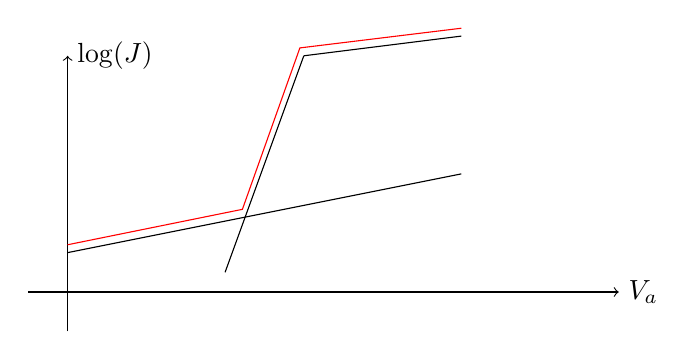
\begin{tikzpicture}
        % disegno asse x
        \draw[->] (-0.5,0)-- (7,0) node[right]{$V_a$};
        % disegno asse y
        \draw[->] (0,-0.5)-- (0,3) node[right]{$\log(J)$};
        %disegno J_SC
        \draw[] (0,0.5)-- (5,1.5);
        %disegno J_0
        \draw[] (2,0.25)-- (3,3);
        %disegno R_serie
        \draw[] (3,3)-- (5,3.25);
        %grafico rosso
        \draw[red] (0,0.6)-- (2.22,1.05)-- (2.95,3.1)-- (5,3.35);
    \end{tikzpicture}
    \caption{Caption}%
    \label{fig:enter_label}
\end{figure}



   \cleardoublepage%
\subsection{GIUNZIONE METALLO-SEMICONDUTTORE: il diodo Schottky}
la giunzione emetallo-semiconduttore è un'eterogiunzione; pertanto è conveniente descrivere il potenziale elettrostatico in funzione del livello del vuoto.\\
Detta $E_w^M$ la funzione lavoro del metallo e $E_w^S$ la funzione lavoro del semiconduttore, si possono verificare quattro casi con i corrispettivi comportamenti elettrici:\\

\noindent\begin{minipage}{0.55\textwidth}
\begin{equation}
    \text{semiconduttore: } n \begin{cases}
    E_w^M > E_w^S & \text{giunzione raddrizzante }\\\\
    E_w^M < E_w^S & \text{giunzione ohmica }
\end{cases}
\end{equation}\\
\begin{equation}
    \text{semiconduttore: } p \begin{cases}
    E_w^M < E_w^S & \text{giunzione raddrizzante }\\\\
    E_w^M > E_w^S & \text{giunzione ohmica }
\end{cases}
\end{equation}
\end{minipage}%
\hfill%
\begin{minipage}{0.3\textwidth}
    \centering
    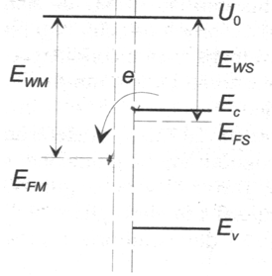
\includegraphics[width=\textwidth]{Immagini_Micro&Nano/Imm_2_Fisica_dei_semiconduttori/giunzione MeSC.PNG}
    \captionof{figure}{caption}
    \label{fig:enter_label}
\end{minipage}

\subsubsection{Semiconduttore di tipo n:}
la prima figura mostra le bande (e quindi i livelli energetici) del metallo e semiconduttore poco prima del contatto.\\
\begin{figure}[hbt!]
    \centering
    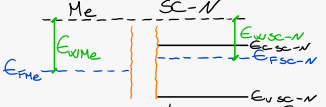
\includegraphics{Immagini_Micro&Nano/Imm_2_Fisica_dei_semiconduttori/giunzioneMeSCn.PNG}
    \caption{Caption}%
    \label{fig:enter_label}
\end{figure}
Al contatto, visto che $E_{wSCn} < E_{wM}$, gli elettroni del semiconduttore tendono a passare nel metallo, dove il livello di fermi è appunto inferiore.
\begin{center}
    \begin{circuitikz}
        %livello fermi metallo
        \draw[dashed] (0,0)--++ (4,0);
        %livello fermi SC
        \draw[dashed] (4,0)--++ (4,0);
        %disegno banda SC
        \draw[domain=0:3.3, samples=400, variable=\x, very thick] plot ({1.2*\x+4},{e^(-1*\x)+0.1});
        \draw[domain=0:3.3, samples=400, variable=\x, very thick] plot ({1.2*\x+4},{e^(-1*\x)-1.9});
        %tratteggi
        \draw[densely dashed] (4,1.1)--++ (0,-3.1);
        \draw[densely dashed] (4,1.1)--++ (4,0);
        %doppie freccie e label
        \draw[>=latex, <->] (6.3,0.25)-- (6.3,1.1);
        \node at (6.3,0.65) [right]{$qV_{bi}$};
        %----
        \draw[>=latex, <->] (3.9,0)-- (3.9,1.1);
        \node at (3.9,0.55) [left]{$q\phi_{Bn}$};
        %----
        \node at (1.7,1.5) []{Metallo};
        \node at (6,1.5) []{SC};
        
        %inserisco elettrone e freccia
        \node at (5,0.8) { \tikz\draw[thick,fill=Ecolour]
        circle (0.13cm) (-0.08,0)-- (0.08,0) ;};
         \node at (4.5,0.9) { \tikz\draw[thick,fill=Ecolour]
        circle (0.13cm) (-0.08,0)-- (0.08,0) ;};
         \node at (5.5,0.6) { \tikz\draw[thick,fill=Ecolour]
        circle (0.13cm) (-0.08,0)-- (0.08,0) ;};

        \draw[-latex] (4.5,1) arc(40:165:1);
        %disegno diodo
        \draw(3,2.5) to [sDo]++ (2,0);
        \node at (3.94,1.85) []{$|||$};
    \end{circuitikz}
\end{center}
La superficie del semiconduttore si svuota dei portatori, mentre nel metallo si forma una regione superficiciale carica negativamente, il cui spessore è trascurabile rispetto alla regione di svuotamento del semiconduttore: La carica sul metallo è virtualmente superficiale.

%
-------------------------------------------------------------\\
Supponiamo di trascurare la corrente dei portatori minoritari. Allora possiamo dire che la condizione di equilibrio termodinamicosi stabilisce quando la corrente totale che attraversa la giunzion è nulla.\\
Questa corrente (costituita quasi totalmente da portatori maggioritari, cioè elettroni) può essere scomposta in due contributi uguali ed opposti:
Corrente associata al flusso di elettroni che vanno dal metallo al semiconduttore e corrente associata al flusso di elettroni che vanno dal semiconduttore al metallo.

Indichiamo con $J_{SM}$ la densità di correntee legata ai portatori che vanno dal semiconduttore al metallo e $J_{MS}$ la densità di corrente legata ai portatori che vanno dal metallo al semiconduttore.
In condizione di equilibrio termodinamico non fluisce corrente, ossia $J_{SM0}=J_{MS0}$.\\
-------------------------------------------------------------\\
Come nel caso di giunzione tra semiconduttori, anche in questo caso si creerà un campo elettrico; il potenziale $\phi$ si può trovare come integrale del campo elettrico lungo x e l'andamento dell'energia si può trovare come $-q\phi$.
A seguito dell'unione dei due mezzi, ai capi della giunzione is forma un potenziale di built-in:
\begin{equation}
    qB_{bi}=E_W^M-E_W^S
\end{equation}
Inltre, all'equilibrio, mentre sul semiconduttore n si sarà instaurata una regione di svuotamento, gli elettroni saranno confinati del metallo a causa di una barriera di potenziale $q\phi_{Bn}=E_W^M-q\alpha$
(dove $\alpha$ è l'affinità elettronica del semiconduttore).\\
\subsubsection{Polarizzazione diretta: $V_A >0$}
per $Va>0$
\begin{center}
    \begin{tikzpicture}
        %livello fermi metallo
        \draw[dashed] (0,0)--++ (4,0);
        %livello fermi SC
        \draw[dashed] (4,0.5)--++ (4,0);
        %disegno banda SC
        \draw[domain=0.63:4, samples=400, variable=\x, very thick] plot ({1.2*\x+3.2},{e^(-1*\x)+0.55});
        \draw[domain=0.63:4, samples=400, variable=\x, very thick] plot ({1.2*\x+3.2},{e^(-1*\x)-1.395});
        
        %tratteggi
        \draw[densely dashed] (4,1.1)--++ (0,-3.1);
        \draw[densely dashed] (4,1.1)--++ (4,0);
        %doppie freccie e label
        \draw[>=latex, <->, red] (4.3,0)--++ (0,0.5);
        \node at (4.3,0.25) [right]{$qV_{A}$};
        %----
        \draw[>=latex, <->] (3.9,0)-- (3.9,1.1);
        \node at (3.9,0.55) [left]{$q\phi_{Bn}$};
        %----
        \draw[>=latex, <->] (6.3,0.65)-- (6.3,1.1);
        \node at (6.3,0.85) [right]{$q(V_{bi}-V_{A})$};
        %----
        \node at (1.7,1.5) []{Metallo};
        \node at (6,1.5) []{SC};
        
        %inserisco elettrone e freccia
        \node at (4.5,0.97) { \tikz\draw[thick,fill=Ecolour]
        circle (0.13cm) (-0.08,0)-- (0.08,0) ;};
        \node at (4.8,0.95) { \tikz\draw[thick,fill=Ecolour]
        circle (0.13cm) (-0.08,0)-- (0.08,0) ;};
         \node at (5,0.85) { \tikz\draw[thick,fill=Ecolour]
        circle (0.13cm) (-0.08,0)-- (0.08,0) ;};

         \draw[-latex] (4.5,1) arc(40:165:1);
         \draw[-latex] (4.7,1.05) arc(40:155:1.2);
    \end{tikzpicture}
\end{center}
Polarizzando direttamente la barriera di potenziale si abbassa. la corrente di diffusione degli elettroni $J_{SM}$ non è più compensata dall'opposta corrente di deriva($J_{SM}>J_{SM0}$.) ma $J_{SM0}=J_{MS0}=J_{MS}$, pertanto $J_{SM0}>J_{MS0}$ e la giunzione conduce corrente dipendente in modo esponenziale dalla tensione applicata (similmente alla giunzione pn).


\subsubsection{Polarizzazione inversa: $V_A <0$}
per $Va<0$
\begin{center}
    \begin{tikzpicture}
        %livello fermi metallo
        \draw[dashed] (0,0)--++ (4,0);
        %livello fermi SC
        \draw[dashed] (4,-0.5)--++ (4,0);
        
        %disegno banda SC
        \draw[domain=0:4.5, samples=400, variable=\x, very thick] plot ({0.9*\x+4},{1.55*e^(-1.05*\x)-0.45});
        \draw[domain=0:4.5, samples=400, variable=\x, very thick] plot ({0.9*\x+4},{1.55*e^(-1.05*\x)-2.295});
        
        %tratteggi
        \draw[densely dashed] (4,1.1)--++ (0,-3.5);
        \draw[densely dashed] (4,1.1)--++ (4,0);
        
        %doppie freccie e label
        \draw[>=latex, <->, red] (3.9,0)--++ (0,-0.5);
        \node at (4,-0.25) [left]{$qV_{A}$};
        %----
        \draw[>=latex, <->] (3.9,0)-- (3.9,1.1);
        \node at (3.9,0.55) [left]{$q\phi_{Bn}$};
        %----
        \draw[>=latex, <->] (6.3,-0.38)-- (6.3,1.1);
        \node at (6.3,0.35) [right]{$q(V_{bi}-V_{A})$};
        %----
        \node at (1.7,1.5) []{Metallo};
        \node at (6,1.5) []{SC};
        
        %inserisco elettrone
        \node at (5.3,0.1) { \tikz\draw[thick,fill=Ecolour]
        circle (0.13cm) (-0.08,0)-- (0.08,0) ;};
        \node at (5.6,0) { \tikz\draw[thick,fill=Ecolour]
        circle (0.13cm) (-0.08,0)-- (0.08,0) ;};
         \node at (6,-0.1) { \tikz\draw[thick,fill=Ecolour]
        circle (0.13cm) (-0.08,0)-- (0.08,0) ;};

    \end{tikzpicture}
\end{center}
Polarizzando inversamente, la barriera di potenziale nel lato semiconduttore si innalza e gli elettroni del semiconduttore vengono respinti verso destra.\\
---si forma quindi un flusso di elettroni dal metallo al semiconduttore che è sostenuto, all'interfaccia metallo-SC, NOP pg 366 fondo...


\begin{figure}[hbt!]
    \centering
    \begin{tikzpicture}[scale=0.5]
             %disegno asse x
            \draw[->] (-2,0) node[anchor=north]{}-- (5,0)
            node[anchor=west]{$x$};
            %disegno asse y
            \draw[->] (0,-3.5)-- (0,3) node[anchor=south west]{$\rho_{fissa}(x)$};
            %disegno grafici
            \draw[thick,pattern=north east lines, pattern color=gray] (0,0)rectangle++ (4,2);
            \draw[-latex, line width=0.75mm] (0,0)--++ (0,-3);
            %label
            \node at (4,0) [anchor=north]{$x_n$};
            \node at (0,2) [anchor=east]{$qN_D$};
            \node at (0,-2.5) [anchor=west]{$-qN_A$};
            \node at (2,1) [red]{$Q^+$};

            %disegno grafico energia
            %disegno asse x
            \draw[->] (-2,-5.5) node[anchor=north]{}-- (5,-5.5)
            node[anchor=west]{$x$};
            %disegno asse y
            \draw[->] (0,-9.5)-- (0,-3.7) node[anchor= west]{$\mathcal{E}(x)$};
            %disegno grafico rosso
            \draw[thick,red] (0,-9)-- (4,-5.5)-- (5,-5.5);
            %label
            \node at (0,-9) [anchor=west]{$\mathcal{E}_{MAX}$};

            %disegno grafico potenziale
            %disegno asse x
            \draw[->] (-2,-12.5) node[anchor=north]{}-- (6,-12.5)
            node[anchor=west]{$x$};
            %disegno asse y
            \draw[->] (0,-15.5)-- (0,-9.7) node[anchor= west]{$\phi(x)$};
            %disegno grafico tensione
            \draw[thick] (0,-12.5).. controls (1.5,-12.5) and (1,-10.7) .. (4,-10.5)--++ (1,0) node[anchor=west]{$V_{bi}$};;
            %disegno grafico potenziale
            \draw[thick] (0,-12.5).. controls (1.5,-12.5) and (1,-15.7) .. (4,-15.5)--++ (1,0);
            \draw[<->] (4,-15.5)-- (4,-12.5);
            \node at (4,-14)[anchor=west]{$q(V_{bi}-V_A)$};
            %label
            \node at (0,-11) [anchor=west]{$\mathcal{E}_{MAX}$};
    \end{tikzpicture}
    \caption{Caption}%
    \label{fig:enter_label}
\end{figure}






manca una figura...\\
\cleardoublepage%
\paragraph{caso giunzione ohmica SCn-Me: $E_w^{Me} > E_w^{SC}$}
%
\begin{figure}[hbt!]
    \centering
    \begin{subfigure}{0.5\textwidth}
        \centering
            \begin{tikzpicture}
            %disegno livello virtuale
            \draw(0,0)--++ (6.5,0);
            %disegno livello fermi per il metallo
            \draw[dashed] (0,-2)--++ (3,0);
            %disegno Banda e fermi del SC
            \draw[] (3,-2.5)--++ (3,0);
            \draw[dashed] (3,-3)--++ (3,0);
            \draw[] (3,-4.5)--++ (3,0);
    
            %livello eergetico metallo
            \draw[>=latex, <->] (1.5,0)--++ (0,-2);
            \node at (1.5,-1) [right]{$E_W^M$};
            %livello energetico SC
            \draw[>=latex, <->] (4.5,0)--++ (0,-3);
            \node at (4.5,-1) [right]{$E_W^S$};
    
            %inserisco elettrone e freccia
            \foreach \pos in {0,0.35}{
            \node at (2.5+ \pos,-1.8) { \tikz\draw[thick,fill=Ecolour]
            circle (0.13cm) (-0.08,0)-- (0.08,0) ;};}
             
             \draw[latex-] (3.5,-2.35) arc(0:75:0.5);
        \end{tikzpicture}
        \caption{Caption}%
        \label{fig:enter_label}\par\vfill
        \end{subfigure}
        %
        \begin{subfigure}{0.5\textwidth}
        \centering
            \begin{tikzpicture}[scale=1]
            %disegno asse x
            \draw[-latex] (-3,0)-- (3,0) node[right]{x};
           % \draw[white]{}(3,0)--++ (0.5,0);
            %disegno asse y
            \draw[-latex] (0,-2)-- (0,2) node[left]{$\rho$};
            %disegno rosso
            \draw[-latex,red,very thick] (0,0)--++ (0,1);
            %disegno blu
        \end{tikzpicture}
        \caption{Caption}%
        \label{fig:enter_label}\par\vfill
        \end{subfigure}
        %
        \begin{subfigure}{0.5\textwidth}
        \centering
            \begin{tikzpicture}
            %disegno asse x
            \draw[dashed] (-3,0)-- (3,0) node[right]{$E_F$};
            %disegno asse y
            \draw[densely dashed] (0,-2)-- (0,2);
            %disegno banda C
            \draw[very thick] (0,-0.4) to [out=60, in=180] (1.5,0.35)--++ (1,0) node[right]{$E_C$};
            %disegno banda V
            \draw[very thick] (0,-1.4) to [out=60, in=180] (1.5,-0.65)--++ (1,0) node[right]{$E_V$};
        \end{tikzpicture}
        \caption{Caption}%
        \label{fig:enter_label}
        \end{subfigure}
        \begin{subfigure}{0.5\textwidth}
        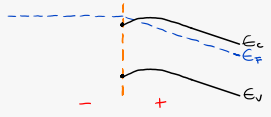
\includegraphics{Immagini_Micro&Nano/Imm_2_Fisica_dei_semiconduttori/giunzione ohmica SCn-Me con Va negativa sul metallo.png}
        \caption{Caption}%
        \label{fig:enter_label}
        \end{subfigure}
        \begin{subfigure}{0.5\textwidth}
        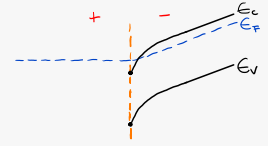
\includegraphics{Immagini_Micro&Nano/Imm_2_Fisica_dei_semiconduttori/giunzione ohmica SCn-Me con Va positiva sul metallo.png}
        \caption{Caption}%
        \label{fig:enter_label}
        \end{subfigure}
\end{figure}
La situazione si analizza come nel caso precedente. Questa volta gli elettroni passeranno dal metallo a semiconduttore.
Questi elettroni si troveranno iniettati in un semicodnuttore in cui sono portatori maggioritari (poi c'è tutto un discorso di debay che non si è spiegato)

non si crea una regione svuotata nè una barriera di potenziale.

Applicando un potenziale positivo al metallo e negativo al semicodnuttore, non essendo presente la regione di svuotamento, si avrà che questo risulta applicato a tutta la giunzione andando a ruotare le bande come nel grafico..
In questo caso gli elettrini nel semiconduttore si possono spostare verso il metallo visto che trovano una banda in discesa.

Se invece si applica una tensione inversa, glie lettroni si potranno spostare dal metallo verso il semiconduttore perchè la banda è in discesa.\\
La corrente che si sviluppa in entrambi i casi è concorde con il valore di Va, per cui questa è una giunzione Ohmica tuttavia nel primo grafico, se il massimo di Ec supera Ef del metallo, allora non è una buona giunzione ohmica

\subsubsection{Giunzione raddrizzante Me-SCp}
\begin{figure}[hbt!]
    \centering
    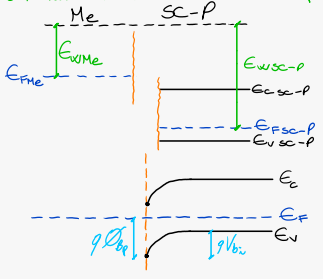
\includegraphics{Immagini_Micro&Nano/Imm_2_Fisica_dei_semiconduttori/giunzione radrizzante MeSCp.png}
    \caption{Giunzione raddrizzante Me-SCp: Diagramma a Bande}%
    \label{fig:Giunzione raddrizzante Me-SCp: Diagramma a Bande}
\end{figure}
%
\cleardoublepage%
%
\subsubsection{Contatti ohmici metallo-semiconduttore}
Per collegare la giunzione PN al mondo esterno è necessario fare delle metallizzazioni. il problema è che facendo qesto si crea un fenomeno fenomeno indesiderato dovuto ad un comportamento parassita.\\
Si supponga infatti, di realizzare un diodo pn e di volerlo connettere al resto del circuito tramite metallizzazione dei contatti.
La metallizzazione dei contatti crea due giunzioni metallo-SC, una con semiconduttore n e l'alto p. ma io sò che se Il lato SCn-metallo realizza una giunzione ohmica allora il contatto p-metallo realizza una giunzione rettificante (e viceversa).\\
La giunzione rettificante è un problema!
\begin{figure}[hbt!]
    \centering
     \begin{circuitikz} [scale=0.75]
        \draw(0,0) 
        to [short]++ (0.5,0) 
        to [short]++ (0,-0.5) rectangle++ (0.35,1)
        to [short]++ (0,-1.5) rectangle++ (2.5,2)
        rectangle++ (2.5,-2)
        to [short]++ (0,0.5) rectangle++ (0.35,1)
        to [short]++ (0,-0.5) to [short]++ (0.5,0);

        %label
        \node at(2.1,0) []{p};
        \node at(4.6,0) []{n};

        % ridisegno le connessioni per poterli colorare
        \draw[fill=gray] (0.5,-0.5) rectangle++ (0.35,1);
        \draw[fill=gray] (5.85,-0.5) rectangle++ (0.35,1);

        
        %disegno circuito equivalente
        \draw(0,-2.25) 
        to [D,bipoles/length=7mm]++ (2,0)
        to [D,bipoles/length=16mm]++ (2.5,0)
        to [R]++ (2,0);
        
    \end{circuitikz}
    \caption{Metallizzazione Me-SC: componenti parassiti}
    \label{fig: Metallizzazione Me-SC: componenti parassiti}
\end{figure}
E' necesario trovare una soluzione per trasformare il contatto rettificante in uno di tipo ohmico.
La soluzione più semplice sarebbe usare un metallo diverso durante la metallizzazione della giunzione drogata p, tuttavia non è una soluzione applicabile perchè La fabbricatura del Wafer non consente di distinguere diversi metalli senza aumentare notevolmente il costo di produzione.\\
Esiste invece una soluzione molto valida che consiste nell'aggiungere una regione fortememnte drogata prima della metallizzazione. Analizzando il caso n, per esempio.
All'aumentare del drogaggio del lato n, lo spessore della regione di carica spaziale diminuisce (è inversamente proporzionale a $\sqrt{N_D}$. Per un drogaggio sufficientemente elevato si ottiene una barriera tanto sottile da consentire il passaggio degli elettroni nelle due direzioni per effetto tunnel.\\

Quindi io applico tra SCn e Metallo una giunzione SCn+. lo strato n+ è così drogato da avere la banda di condizione sotto al livello di fermi, per cui si ottiene il diagramma a bande:

\begin{figure}[hbt!]
    \centering
    \begin{circuitikz}
        \draw(0.85,0.5) 
        to [short]++ (0,-1.5) rectangle++ (2.5,2)
        rectangle++ (1,-2)
        to [short]++ (0,0.5) rectangle++ (0.35,1)
        to [short]++ (0,-0.5) to [short]++ (0.5,0);

        %label
        \node at(2.1,0) []{n};
        \node at(3.9,0) []{$n^+$};

        % ridisegno le connessioni per poterli colorare
        \draw[fill=gray] (4.35,-0.5) rectangle++ (0.35,1);
        
        %disegno asse x
        %disegno asse y
        %disegno tratteggi
        \draw[densely dashed] (0.5,-3)--++ (4.75,0);
        \draw[densely dashed] (3.35,-1)--++ (0,-3.25);
        \draw[densely dashed] (4.35,-1)--++ (0,-3.25);
        \draw[densely dashed] (4.7,-0.5)--++ (0,-3.75);
        %disegno grafico
        \draw[very thick, red] (1,-2.5) node[left]{$E_C$}-- (2.9,-2.5)..controls (3.55,-2.5) and (3.3,-4).. (3.8,-4)
                             ..controls (4.3,-4) and (4.2,-1.5).. (4.35,-1.5);
        %label
        \draw[latex-latex,blue,thick] (4.35,-1.5) node[anchor=north west]{$\phi_{bn}$}-- (4.35,-3);
        %frecce
        \draw[-stealth,decorate,decoration={snake,amplitude=3pt,pre length=2pt,post length=3pt}] (5,-2.2) -- ++ (-2,0);
        \draw[stealth-,decorate,decoration={snake,amplitude=3pt,pre length=2pt,post length=3pt}] (5,-2.4) -- ++ (-2,0);

    \end{circuitikz}
    \caption{Metallizzazione Me-SC: drogaggio intermedio n+}
    \label{fig:Metallizzazione Me-SC: drogaggio intermedio n+}
\end{figure}


\begin{figure}[hbt!]
    \centering
     \begin{circuitikz}[scale=0.75]
        \draw(0,0) 
        to [short]++ (0.5,0) 
        to [short]++ (0,-0.5) rectangle++ (0.35,1)
        to [short]++ (0,-1.5) rectangle++ (2.5,2)
        rectangle++ (2.5,-2)
        rectangle++ (1,2)
        to [short]++ (0,-0.5) rectangle++ (0.35,-1)
        to [short]++ (0,+0.5) to [short]++ (0.5,0);

        %label
        \node at(2.1,0) []{p};
        \node at(4.6,0) []{n};
        \node at(6.4,0) []{$n^+$};

        % ridisegno le connessioni per poterli colorare
        \draw[fill=gray] (0.5,-0.5) rectangle++ (0.35,1);
        \draw[fill=gray] (6.85,-0.5) rectangle++ (0.35,1);

    \end{circuitikz}
    \caption{Metallizzazione Me-SC corretto}
    \label{fig: Metallizzazione Me-SC corretto}
\end{figure}
In questo modo la banda di conduzione vicino al metallo assume la forma a barriera di potenziale di spessore motlo sottile, favorendo il passaggio per effetto tunnel.\\
Gli elettroni possono attraversare questa giunzione per qualsiasi Va applicata come se fosse una giunzione ohmica.
\begin{figure}[hbt!]
    \centering
     \begin{circuitikz} [scale=0.75]
        \draw(0,0) 
        to [short]++ (0.5,0) 
        to [short]++ (0,-0.5) rectangle++ (0.35,1)
        to [short]++ (0,-1.5) rectangle++ (2.5,2)
        rectangle++ (2.5,-2)
        to [short]++ (0,0.5) rectangle++ (0.35,1)
        to [short]++ (0,-0.5) to [short]++ (0.5,0);

        %label
        \node at(2.1,0) []{p};
        \node at(4.6,0) []{n};

        % ridisegno le connessioni per poterli colorare
        \draw[fill=gray] (0.5,-0.5) rectangle++ (0.35,1);
        \draw[fill=gray] (5.85,-0.5) rectangle++ (0.35,1);
        
        %disegno circuito equivalente
        \draw(0,-2.25) 
        to [R]++ (2,0)
        to [D,bipoles/length=16mm]++ (2.5,0)
        to [R]++ (2,0);
        
    \end{circuitikz}
    \caption{Metallizzazione Me-SC corretto: parassiti ohmici}
    \label{fig: Metallizzazione Me-SC corretto: parassiti ohmici}
\end{figure}
%
\cleardoublepage%
%
\subsection{Capacità di giunzione per un diodo Schottky}
Il diodo schottky ha una capacità di diffusione nulla ($C_D=0$) ed una capacità di giunzione $C_j$ pari a quella di un semiconduttore PN con p molto drogato.\\
%
\noindent\begin{minipage}{0.5\textwidth}% adapt widths of minipages to your needs
La carica dovuta alla zona di svuotamento sarà
\begin{align}
    Q_j&=q\ N_D\ x_n=A \sqrt{q\ \mathcal{E}\ N_D\ 2(V_{bi}-V_A) }\\
    \intertext{Per cui la capacità di giunzione sarà:}
    C_j&=\left| \dfrac{dQ_j}{dV_A}\right|= A \sqrt{ \dfrac{q\ \mathcal{E}\ N_D}{2(V_{bi}-V_A)}}
\end{align}
\end{minipage}%
\hfill%
\begin{minipage}{0.3\textwidth}
    \begin{tikzpicture}[scale=0.5,transform shape]
             %disegno asse x
            \draw[->] (-2,0) node[anchor=north]{}-- (5,0)
            node[anchor=west]{$x$};
            %disegno asse y
            \draw[->] (0,-3.5)-- (0,3) node[anchor=south west]{$\rho_{fissa}(x)$};
            %disegno grafici
            \draw[thick,pattern=north east lines, pattern color=gray] (0,0)rectangle++ (4,2);
            \draw[-latex, line width=0.75mm,blue] (0,0)--++ (0,-3);
            %label
            \node at (4,0) [anchor=north]{$x_n$};
            \node at (0,2) [anchor=east]{$qN_D$};
            \node at (0,-2.5) [anchor=west]{$-qN_A$};
            \node at (2,1) [red]{$Q^+$};

            %disegno grafico energia
            %disegno asse x
            \draw[->] (-2,-5.5) node[anchor=north]{}-- (5,-5.5)
            node[anchor=west]{$x$};
            %disegno asse y
            \draw[->] (0,-9.5)-- (0,-3.7) node[anchor= west]{$\mathcal{E}(x)$};
            %disegno grafico rosso
            \draw[thick,red] (0,-9)-- (4,-5.5)-- (5,-5.5);
            %label
            \node at (0,-9) [anchor=west]{$\mathcal{E}_{MAX}=\dfrac{q\ N_D}{\varepsilon}x_n$};
            %disegno freccia del campo elettrico
            \draw[latex-] (0,-5)-- (4,-5) node[anchor= west]{$\mathcal{E}(x)$};
            
            %disegno grafico potenziale
            %disegno asse x
            \draw[->] (-2,-12.5) node[anchor=north]{}-- (6,-12.5)
            node[anchor=west]{$x$};
            %disegno asse y
            \draw[->] (0,-13.5)-- (0,-9.7) node[anchor= west]{$\phi(x)$};
            %disegno grafico tensione
            \draw[thick] (0,-12.5).. controls (1.5,-12.5) and (1,-10.7) .. (4,-10.5)--++ (1,0) node[anchor=west]{$q(V_{bi}-V_A)$};;
            
    \end{tikzpicture}
\end{minipage}
\begin{riepilogo}
    
\end{riepilogo}
\cleardoublepage%